% Options for packages loaded elsewhere
\PassOptionsToPackage{unicode}{hyperref}
\PassOptionsToPackage{hyphens}{url}
\PassOptionsToPackage{dvipsnames,svgnames,x11names}{xcolor}
\PassOptionsToPackage{space}{xeCJK}
\documentclass[
  12pt,
  a4paper]{ctexbook}
\usepackage{xcolor}
\usepackage[top=2.5cm,bottom=2.5cm,left=3cm,right=2.6cm]{geometry}
\usepackage{amsmath,amssymb}
\setcounter{secnumdepth}{5}
\usepackage{iftex}
\ifPDFTeX
  \usepackage[T1]{fontenc}
  \usepackage[utf8]{inputenc}
  \usepackage{textcomp} % provide euro and other symbols
\else % if luatex or xetex
  \usepackage{unicode-math} % this also loads fontspec
  \defaultfontfeatures{Scale=MatchLowercase}
  \defaultfontfeatures[\rmfamily]{Ligatures=TeX,Scale=1}
\fi
\usepackage{lmodern}
\ifPDFTeX\else
  % xetex/luatex font selection
  \ifXeTeX
    \usepackage{xeCJK}
    \setCJKmainfont[]{Songti SC}
    \setCJKsansfont[]{Hiragino Sans GB}
  \fi
  \ifLuaTeX
    \usepackage[]{luatexja-fontspec}
    \setmainjfont[]{Songti SC}
  \fi
\fi
% Use upquote if available, for straight quotes in verbatim environments
\IfFileExists{upquote.sty}{\usepackage{upquote}}{}
\IfFileExists{microtype.sty}{% use microtype if available
  \usepackage[]{microtype}
  \UseMicrotypeSet[protrusion]{basicmath} % disable protrusion for tt fonts
}{}
\usepackage{setspace}
\makeatletter
\@ifundefined{KOMAClassName}{% if non-KOMA class
  \IfFileExists{parskip.sty}{%
    \usepackage{parskip}
  }{% else
    \setlength{\parindent}{0pt}
    \setlength{\parskip}{6pt plus 2pt minus 1pt}}
}{% if KOMA class
  \KOMAoptions{parskip=half}}
\makeatother
\usepackage{longtable,booktabs,array}
\newcounter{none} % for unnumbered tables
\usepackage{calc} % for calculating minipage widths
% Correct order of tables after \paragraph or \subparagraph
\usepackage{etoolbox}
\makeatletter
\patchcmd\longtable{\par}{\if@noskipsec\mbox{}\fi\par}{}{}
\makeatother
% Allow footnotes in longtable head/foot
\IfFileExists{footnotehyper.sty}{\usepackage{footnotehyper}}{\usepackage{footnote}}
\makesavenoteenv{longtable}
\setlength{\emergencystretch}{3em} % prevent overfull lines
\sloppy
\setlength{\parindent}{2em}
\setlength{\parskip}{0pt}
\renewcommand{\arraystretch}{1.22}
\setlength{\tabcolsep}{4.8pt}
\usepackage{tikz}
\usetikzlibrary{arrows.meta,calc,decorations.pathreplacing,positioning,fit,matrix}
\usepackage{colortbl}
\usepackage{caption}
\usepackage{etoolbox}
\usepackage{float}
\usepackage{flafter}
\definecolor{ThesisNavy}{HTML}{244A64}
\definecolor{ThesisBlue}{HTML}{4E7896}
\definecolor{ThesisTeal}{HTML}{4F8A83}
\definecolor{ThesisRust}{HTML}{B7654A}
\definecolor{ThesisGold}{HTML}{C49A45}
\definecolor{ThesisLavender}{HTML}{80728F}
\definecolor{ThesisInk}{HTML}{25333C}
\definecolor{ThesisGrid}{HTML}{D8E0E5}
\definecolor{ThesisPale}{HTML}{EDF3F6}
\tikzset{every picture/.style={line cap=round,line join=round},thesisbox/.style={draw=ThesisNavy,line width=.65pt,rounded corners=2pt,fill=ThesisPale,text=ThesisInk,align=center,inner xsep=8pt,inner ysep=5pt},thesisarrow/.style={-{Stealth[length=2.2mm]},line width=.75pt,draw=ThesisNavy}}
\captionsetup{font=small,labelfont=bf,labelsep=quad,skip=6pt}
\renewcommand{\thefigure}{\thechapter-\arabic{figure}}
\renewcommand{\thetable}{\thechapter-\arabic{table}}
\setlength{\LTpre}{6pt}
\setlength{\LTpost}{9pt}
\AtBeginEnvironment{longtable}{\small\arrayrulecolor{ThesisNavy!55}}
\ctexset{chapter={beforeskip=18pt,afterskip=20pt},section={beforeskip=16pt,afterskip=10pt},subsection={beforeskip=12pt,afterskip=7pt}}
\let\cleardoublepage\clearpage
\providecommand{\tightlist}{%
  \setlength{\itemsep}{0pt}\setlength{\parskip}{0pt}}
\usepackage{bookmark}
\IfFileExists{xurl.sty}{\usepackage{xurl}}{} % add URL line breaks if available
\urlstyle{same}
\hypersetup{
  pdftitle={全国中学生物理竞赛复赛理论试题的科学思维要求及教学设计启示},
  pdfauthor={董兴习},
  colorlinks=true,
  linkcolor={black},
  filecolor={Maroon},
  citecolor={Blue},
  urlcolor={black},
  pdfcreator={LaTeX via pandoc}}

\title{全国中学生物理竞赛复赛理论试题的\\[0.45em]科学思维要求及教学设计启示}
\author{董兴习}
\date{2026年7月}

\begin{document}
\frontmatter
\maketitle

{
\setcounter{tocdepth}{2}
\tableofcontents
}
\setstretch{1.5}
\mainmatter
\chapter*{摘要}\addcontentsline{toc}{chapter}{摘要}\label{ux6458ux8981}

本研究以第35至42届全国中学生物理竞赛复赛理论试题为对象，分析模型建构、科学推理、科学论证和质疑创新四维科学思维要求，并据此提出教学设计启示。研究以具有独立作答目标的小问为分析单位，建立221个分析单元，分别判断四个维度是否出现及其SOLO启发的任务结构等级，形成884条V3唯一编码记录。每条记录均保留题干、参考解答、证据位置和相邻等级排除理由，经作者逐题实质复核后，由同一版本编码表生成维度出现、等级构成、组合和届次描述统计。结果显示，模型建构、科学推理、科学论证和质疑创新分别出现于202、221、36和2个单元，占91.40\%、100.00\%、16.29\%和0.90\%。在相应维度已经出现的单元中，模型建构L1、L2、L3分别为9、77、116个，科学推理分别为13、69、139个，科学论证分别为14、16、6个，质疑创新仅有2个L2单元，四个维度均未出现L4。科学推理的二元指标在本样本中达到饱和，其区分信息主要来自等级及具体关系结构，不能由100\%的出现率推断所有小问结构相同或学生具有相应能力。模型建构与科学推理同时出现于202个单元，四维同时出现仅2个单元。六个典型案例进一步呈现条件---关系链、状态分类与比较、近似条件建模、同对象比较、多对象约束和阈值判断等任务结构，并形成``任务结构---学习任务---支架---可观察产出---反馈要点''的教学设计链条。研究将小问级描述统计与具体物理机制相互印证，为复赛试题研究和竞赛教学设计提供可追溯依据；结论只描述试题及参考解答呈现的任务要求，不直接等同于学生实际能力或教学效果。

关键词：物理竞赛；科学思维；内容分析；任务认知要求；教学设计

\chapter*{ABSTRACT}\addcontentsline{toc}{chapter}{ABSTRACT}\label{abstract}

This study investigates the scientific-thinking requirements of the
theoretical problems in the second-round papers from the 35th to the
42nd editions of the National Physics Competition for High School
Students in China and derives implications for instructional design.
Subquestions with independent response goals yielded 221 analytical
units and 884 records in the V3 unique coding dataset. For each unit,
content analysis identified the presence of model construction,
scientific reasoning, scientific argumentation, and questioning and
innovation, together with their SOLO-inspired task-structure levels.
Each record retained evidence from the item statement and reference
solution, source locations, and the rationale for excluding adjacent
levels. Following an item-by-item substantive review by the author, all
descriptive tables and figures were generated from the same
version-controlled dataset. Model construction, scientific reasoning,
scientific argumentation, and questioning and innovation occurred in
202, 221, 36, and 2 units, accounting for 91.40\%, 100.00\%, 16.29\%,
and 0.90\% of the sample. Among units in which each dimension was
present, the L1/L2/L3 counts were 9/77/116 for model construction,
13/69/139 for scientific reasoning, and 14/16/6 for scientific
argumentation; both instances of questioning and innovation were coded
L2, and no L4 instance occurred in any dimension. The binary
scientific-reasoning indicator was saturated in this sample, so its
discriminating information lies in task-structure levels and specific
physical relations rather than in the 100\% presence rate. Model
construction and scientific reasoning co-occurred in 202 units, whereas
all four dimensions co-occurred in only 2 units. Six representative
cases revealed condition-relation chains, state classification and
comparison, approximation-based modeling, same-object comparison,
multi-object constraints, and threshold judgment. These structures
supported an instructional-design chain linking task structure, learning
task, scaffold, observable product, and feedback focus. The findings
connect subquestion-level descriptive statistics with concrete physical
mechanisms and describe requirements represented by the items and
reference solutions rather than students' actual capabilities or
instructional effectiveness.

Keywords: physics competition; scientific thinking; content analysis;
task cognitive requirements; instructional design

\chapter{绪论}\label{ux7eeaux8bba}

\section{研究背景与问题提出}\label{ux7814ux7a76ux80ccux666fux4e0eux95eeux9898ux63d0ux51fa}

\subsection{科学思维与竞赛试题分析}\label{ux79d1ux5b66ux601dux7ef4ux4e0eux7adeux8d5bux8bd5ux9898ux5206ux6790}

普通高中物理课程改革将科学思维作为物理学科核心素养的重要组成部分，并将模型建构、科学推理、科学论证、质疑创新列为科学思维的重要表现。\textsuperscript{[1]}
课程标准为本研究选择科学思维维度、界定分析内容提供了理论依据；在此基础上，本文结合复赛试题的题干、参考解答和编码规则开展具体分析。

复赛试题分析不宜只停留在知识点、题型或难度描述，还需要关注试题实际要求解题者完成的认知活动：如何抽象物理模型，如何组织条件链，如何说明边界条件，如何在陌生情境中迁移或修正已有模型。因此，本文从科学思维维度和任务认知结构要求两个层面分析复赛试题。

本文整理第35至42届全国中学生物理竞赛复赛试题与参考答案，以具有独立作答目标的小问为基本单位，共形成221个分析单元和884条维度编码记录。每条记录均对应题干触发语、参考解答关键步骤和证据定位，第四章据此呈现维度分布、等级构成、组合关系与届次描述。相关统计描述的是试题任务要求，不用于推断学生能力、教学效果或命题趋势。

全国中学生物理竞赛复赛试题具有综合性强、情境多样、推导链条长的特点。一道题目往往同时包含物理对象的抽象、条件与边界的确定、规律关系的组织、数学工具的使用以及结果的解释。若仅从力学、电磁学、光学或近代物理等知识模块分类，能够说明题目涉及的内容范围，却难以揭示解题者在完成任务时需要进行何种思维活动；若只依据题量、分值、公式数量或计算长度判断难度，也容易忽略不同题目在模型设定、推理组织和论证要求上的差异。

以任务结构为中心的分析能够补充这一不足。它不把竞赛题简化为``考查某一知识点''，而是考察题干与参考解答共同要求解题者完成的活动：是否需要从复杂情境中确定研究对象和理想化条件，是否需要将多个规律与条件组织为关系链，是否需要比较不同情形或说明结论的适用范围，是否需要修正假设或构造新的方案。这样的视角既能保持物理内容的具体性，也能把不同题材中的相似思维要求识别出来。

复赛题的教学价值也由此得到更细致的理解。竞赛训练当然需要掌握较高水平的物理知识与数学工具，但训练过程不应只表现为``看懂答案---模仿步骤---完成计算''。当教师能够识别一道题中最关键的条件、模型、推理或论证环节时，就可以设计相应的追问、书面产出和反馈方式，使学生不仅获得结论，也理解结论如何由条件和规律共同支撑。本文正是在这一背景下，尝试从试题分析中提炼竞赛教学设计启示。

由此，本研究的问题意识可以概括为：复赛理论试题要求解题者进行怎样的科学思维活动，如何把这些要求转化为可编码、可复核的分析框架，又如何依据反复出现的任务结构设计竞赛教学中的学习任务、支架、可观察产出与反馈要点。

\section{核心概念与研究边界}\label{ux6838ux5fc3ux6982ux5ff5ux4e0eux7814ux7a76ux8fb9ux754c}

\subsection{核心概念界定}\label{ux6838ux5fc3ux6982ux5ff5ux754cux5b9a}

本研究以模型建构、科学推理、科学论证、质疑创新四个维度组织试题分析。这一维度结构具有课程标准依据，\textsuperscript{[1]}
每个维度均通过编码手册、边界案例、匿名回填比较和证据复核落实为可操作的判定规则。

本研究中的``认知要求''指试题及参考解答对解题者提出的任务要求，而不是学生实际达到的能力水平。换言之，论文分析的是``题目要求完成什么样的思维活动''，不是``学生已经具备什么能力''。科学推理和科学思维测评研究也提示，学生能力判断需要测评任务、作答数据和模型检验，不能由试题文本分析直接推出。\textsuperscript{[2, 3]}
没有学生作答、访谈、课堂观察或测评数据时，不能把试题编码结果解释为学生科学思维水平。

本研究中的``SOLO启发等级''只用于描述某一科学思维维度出现时的任务结构复杂性。本文使用``SOLO启发的任务认知结构要求等级''这一表述，不将试题直接等同于学生学习结果等级。

本研究中的``教学设计启示''指由试题任务结构提出学习任务、支架、可观察产出和反馈方式。科学论证教学研究和国际科学实践框架可以为``任务、支架、评价对象''的设计提供参照，\textsuperscript{[4, 5]}
但不能据此认定教学策略已经有效。本文未采集教师访谈、问卷、课堂记录、学生作品或前后测数据，因此第五章提出的是基于试题分析的教学设计建议，不报告学生表现或教学效果。

\section{国内外研究现状}\label{ux56fdux5185ux5916ux7814ux7a76ux73b0ux72b6}

\subsection{研究视角与文献基础}\label{ux7814ux7a76ux89c6ux89d2ux4e0eux6587ux732eux57faux7840}

本研究的文献综述围绕四组材料展开。第一组是课程标准和科学思维理论，用于说明以模型建构、科学推理、科学论证、质疑创新组织分析的依据。第二组是SOLO理论及任务分析相关研究，用于界定SOLO作为任务认知结构等级启发来源的适用范围。第三组是物理竞赛试题研究，用于比较既有研究在样本范围、分析单位和分析视角上的处理方式。第四组是内容分析、编码一致性和教学设计研究，用于支撑编码流程、质量检验和结果解释；其中编码一致性按变量呈现，并保留分歧处理记录。\textsuperscript{[6]}

现有研究分别提供了科学思维要素、任务结构解释、内容分析程序和教学设计参照。\textsuperscript{[1, 2, 3, 4, 5, 6]}
这些研究提示，有必要从科学思维维度和任务结构角度补充复赛小问级证据；本文据此提出研究问题，而不把这一判断表述为对既有研究的穷尽性否定。

因此，本章以研究问题所需的文献脉络为主，第二章再围绕科学思维、SOLO启发的任务结构、内容分析与教学设计展开系统讨论，并将每类文献放在其能够支撑的论证位置上。

\subsection{国内物理竞赛试题研究}\label{ux56fdux5185ux7269ux7406ux7adeux8d5bux8bd5ux9898ux7814ux7a76}

国内关于中学生物理竞赛试题的研究已经形成若干较有代表性的路径。第一类研究以典型题为对象，从核心素养或科学思维角度分析题目情境、物理过程与解答要求。此类研究能够较细致地揭示一道或若干道题目中蕴含的物理思想，但样本数量较少，结论主要适用于所选案例。第二类研究以若干届试卷为样本，围绕题型、知识板块、分值、题量或考查内容进行统计，能够展示试卷结构的总体特征，却较少进入小问层面的任务结构。第三类研究引入SOLO分类或综合难度模型，尝试用明确的分类规则分析复赛理论题，为竞赛试题的系统研究提供了重要参照。\textsuperscript{[13, 15, 16, 17]}

预赛研究通常重视题型、知识分布和典型题的素养表现。凌国亮等以预赛典型题及其解答过程讨论数理核心素养，强调从题目条件、物理规律和推导过程理解考查要求；另有研究以多届预赛卷为材料，对题型、分值、知识板块和考查内容进行量化描述。这些研究说明，竞赛试题分析既可以从具体题目切入，也可以从多届试卷结构切入。由于预赛与复赛在任务开放度、计算深度和题目组织方式上存在差异，预赛研究的统计口径不能直接替代复赛小问级分析，但其关于语料范围、分析变量和规则公开的处理具有方法启示。\textsuperscript{[15, 16]}

复赛研究更接近本研究的对象。龚枭以第26至35届复赛理论题为材料，使用SOLO分类理论组织试题分析；张豇萌以第34至38届复赛理论题为样本，依据综合难度模型对试题进行统计。两项研究共同表明，复赛理论题可以进行跨届、系统的文本研究，也需要说明样本范围、分析单位和赋值规则。二者的研究重点分别在整题SOLO分类和综合难度构成，而本文将独立小问作为基本单位，分别记录模型建构、科学推理、科学论证和质疑创新的出现及其任务结构要求。这样的差异并非否定既有研究，而是将关注点从``题目总体属于何种类型或难度''转向``题目要求解题者完成哪些思维活动''。\textsuperscript{[13, 17]}

唐路的研究还将复赛、决赛题目统计与成绩资料、案例分析并置，提示竞赛题研究中存在题目文本、试题统计和参赛者表现等多种证据来源。不同证据回答的问题不同：题目与参考解答能够说明任务要求，成绩资料能够呈现特定样本的作答表现，访谈或课堂资料才能进一步讨论学习过程。本文聚焦前一类证据，因此不将试题编码结果延伸为地区成绩、学生能力或教学效果的结论。\textsuperscript{[14]}

\subsection{本研究的切入点}\label{ux672cux7814ux7a76ux7684ux5207ux5165ux70b9}

综合已有研究可以发现，竞赛试题研究正在从知识点归类和试卷结构统计走向更细致的任务分析，但在复赛语料中，仍有必要进一步说明分析单位、判定依据和任务结构之间的关系。以整题为单位时，同一题中不同小问可能被合并为同一种难度或层次；以分值或公式数量作为主要指标时，模型简化、条件组织、论证说明和方案比较等差异也容易被遮蔽。小问级分析能够保留这些差异，使不同维度在同一题内的组合关系得到呈现。

从研究对象、分析单位与结果解释三个方面比较，现有路径各有适用范围。以典型题为中心的研究有利于深入说明一个物理问题中概念、规律和情境之间的联系，但其结论通常不宜外推到整套试题；以整卷或整题为单位的统计便于描绘题型、知识模块与分值结构，却容易把同一大题内部由基础推演到条件讨论的层次变化压缩为一个标签；以综合难度模型为基础的研究能够提供多指标比较，却不能自动回答某一小问究竟要求解题者进行建模、论证还是方案调整。本文并不试图以一种分类替代上述研究，而是把独立小问作为观察窗口：统计结果首先回答``哪些任务要求出现''，随后再回到题干和解答说明``这些要求如何在物理求解中发生''。

这一选择也影响论文对``差异''的理解。若某一知识模块中科学论证记录较多，本文不会把它解释为该模块天然更高级，而会进一步追问：该模块的题目是否较多出现比较、极限、近似或适用范围说明；若某一届质疑创新记录较少，也不能据此判断命题质量高低，而应考察该届题目是否更多在已给模型中展开推演。换言之，统计表提供的是检索和比较的入口，物理任务的具体组织才是解释的落点。这样的处理既保留跨届语料的整体视野，也避免让百分比脱离题目本身。

因此，本文的研究定位包括三个方面：其一，以第35至42届复赛试题的独立小问为分析单位，形成跨届而颗粒度较细的语料；其二，以科学思维四维度和SOLO启发的任务结构等级构成两层分析框架，避免将知识内容、难度和思维要求混为一谈；其三，在描述性统计之外回到题干与参考解答，选取具有代表性的任务结构案例，提出面向竞赛教学的任务、支架和评价建议。上述定位使本文既保持竞赛试题研究的系统性，也保留对具体物理任务的解释力。

本文所说的教学设计启示不是把统计比例逐条改写成教学口号。真正能够进入教学设计的是统计背后反复出现的任务结构：例如，若一个小问的关键在于把限制条件引入关系链，教学中就应让学生呈现条件如何进入推导；若一个小问的关键在于状态分类，教学中就应让学生说明分类依据与比较对象；若一个小问依赖近似假设，教学中就应让学生解释忽略什么、保留什么以及结论适用到何处。这样的设计路径把研究结果、学生可见产出和教师反馈连接起来，同时不把尚未收集的学生表现预先写入研究结论。

\section{研究问题}\label{ux7814ux7a76ux95eeux9898}

\subsection{研究问题设计}\label{ux7814ux7a76ux95eeux9898ux8bbeux8ba1}

结合研究语料、分析方法和证据范围，本研究回答以下问题：

\begin{enumerate}
\def\labelenumi{\arabic{enumi}.}
\tightlist
\item
  如何构建适用于全国中学生物理竞赛复赛试题的科学思维认知要求分析框架？
\item
  第35至42届复赛试题在模型建构、科学推理、科学论证和质疑创新四个维度上呈现出怎样的任务要求？
\item
  这些试题在认知结构要求等级、维度组合和典型题设机制上有哪些特征？
\item
  第35至42届复赛试题的科学思维要求在届次层面呈现怎样的样本内部差异？
\item
  基于复赛试题中反复出现的任务结构，可以提出哪些竞赛教学设计启示？
\end{enumerate}

上述问题中，第2至第4个问题基于编码表作描述性回答，不据此推断学生能力、命题长期趋势或因果关系。第5个问题着重回答``如何设计''，不以试题分析代替教学效果检验。

\subsection{研究问题之间的逻辑关系}\label{ux7814ux7a76ux95eeux9898ux4e4bux95f4ux7684ux903bux8f91ux5173ux7cfb}

五个研究问题不是彼此孤立的。第一个问题解决``用什么语言分析试题''的问题：只有先明确四个维度分别观察什么、等级如何理解，后续的统计才有共同口径。第二个问题回答全样本中各类任务要求的基本分布，第三个问题进一步考察这些要求在等级和组合上的结构特征，第四个问题把这种结构放回八届样本中呈现其描述性背景。第五个问题则把统计和案例中已经识别出的任务结构，转化为可安排、可观察的教学活动。

这种由框架到分布、由分布到案例、再由案例到教学设计的顺序，能够避免两种常见的跳跃。其一，不能只凭某一题``综合''或``新颖''就断言它具有某一种科学思维要求；任务的判定仍需回到题干和参考解答。其二，不能把总体百分比直接翻译成教学结论；例如，某一维度出现较多，只说明相应任务要求在当前语料中较常见，还需要结合其具体表现形式设计学习任务。研究问题之间的衔接，正是为了使结论既保留总体视野，也不脱离物理问题本身。

\subsection{各研究问题的回答依据}\label{ux5404ux7814ux7a76ux95eeux9898ux7684ux56deux7b54ux4f9dux636e}

第一个问题主要依据课程标准中的科学思维要素、SOLO启发的任务结构理解、编码手册及边界案例回答。其重点不是为四个维度赋予抽象定义，而是说明何种题干要求和解答步骤可以作为判定依据。第二至第四个问题主要依据221个分析单元的V3唯一编码记录、元数据索引和描述统计表回答，其中统计数字必须与题干和解答证据相互对应。第五个问题以典型案例中可见的条件识别、模型组织、关系推演、比较说明和边界核对为依据，形成任务、支架和评价产出的设计建议。

不同问题所依托的材料不同，结论强度也应有所区别。全样本编码表可以支持``某种任务要求在本语料中出现多少次''的描述；典型案例可以支持``这种要求在某一物理任务中如何实现''的解释；教学设计材料可以支持``可据此设计何种学习产出''的建议。本文据此将试题任务要求、学生实际表现和教学效果分开处理，使每一部分的论证都有清楚的材料来源。

\section{研究内容、方法和技术路线}\label{ux7814ux7a76ux5185ux5bb9ux65b9ux6cd5ux548cux6280ux672fux8defux7ebf}

\subsection{研究内容与技术路线}\label{ux7814ux7a76ux5185ux5bb9ux4e0eux6280ux672fux8defux7ebf}

本研究采用``复赛试题内容分析---典型机制解释---教学设计启示''的路线。论文以第35至42届复赛试题为语料，将典型试题机制分析与基于任务结构的教学设计建议相衔接；教学设计部分提出可实施的任务结构，不作教学效果验证。

研究内容包括五部分。第一，建立复赛试题小问级语料库，记录题号、小问、页码、知识模块、情境、表征和数学工具等信息。第二，基于课程标准、SOLO启发等级和内容分析方法，形成科学思维维度与任务认知结构等级的编码框架。第三，在早期编码比较与边界修订的基础上，按V3编码手册重新形成候选记录，由作者逐题复核并生成884行唯一编码表。第四，以该唯一编码表生成维度出现、等级、组合、共现和届次分布的描述性分析。第五，依据典型任务结构提出竞赛教学中的任务、支架、可观察产出和反馈建议。\textsuperscript{[4, 5]}

技术路线如下：

\begin{figure}[H]
\centering
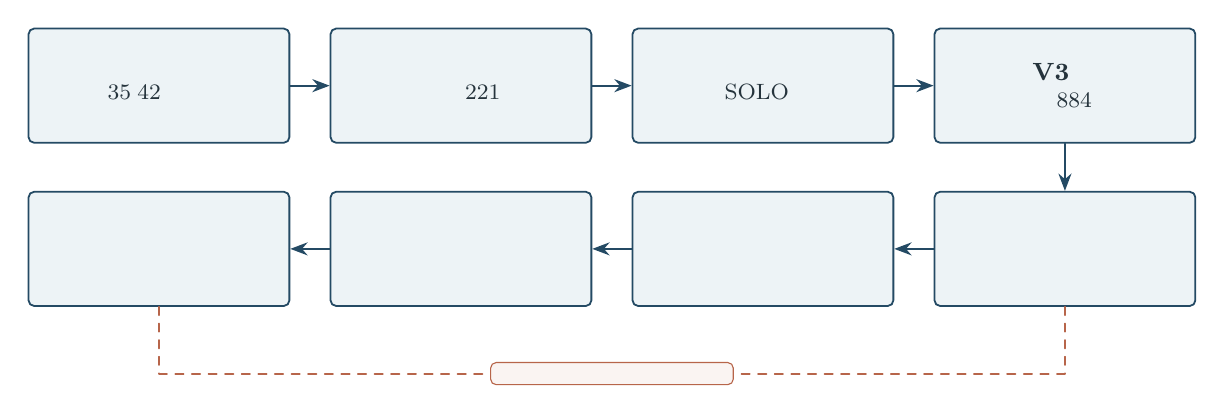
\begin{tikzpicture}[
  node distance=6mm and 5mm,
  every node/.style={font=\small},
  stage/.style={thesisbox,text width=2.75cm,minimum height=1.45cm}
]
  \node[stage] (corpus) {\textbf{试题语料}\\[-1pt]\footnotesize 第35至42届复赛题与参考解答};
  \node[stage,right=of corpus] (unit) {\textbf{分析单位}\\[-1pt]\footnotesize 按独立作答目标拆分为221个小问};
  \node[stage,right=of unit] (framework) {\textbf{分析框架}\\[-1pt]\footnotesize 四维度与SOLO启发结构等级};
  \node[stage,right=of framework] (coding) {\textbf{V3全量编码}\\[-1pt]\footnotesize 四维展开形成884条记录};
  \node[stage,below=of coding] (quality) {\textbf{质量控制}\\[-1pt]\footnotesize 逐题复核、证据校验与版本验收};
  \node[stage,left=of quality] (statistics) {\textbf{描述分析}\\[-1pt]\footnotesize 出现比例、等级构成与共现关系};
  \node[stage,left=of statistics] (cases) {\textbf{案例解释}\\[-1pt]\footnotesize 还原条件、模型、推理与边界机制};
  \node[stage,left=of cases] (teaching) {\textbf{教学设计}\\[-1pt]\footnotesize 形成任务、支架与可观察产出};
  \draw[thesisarrow] (corpus) -- (unit);
  \draw[thesisarrow] (unit) -- (framework);
  \draw[thesisarrow] (framework) -- (coding);
  \draw[thesisarrow] (coding) -- (quality);
  \draw[thesisarrow] (quality) -- (statistics);
  \draw[thesisarrow] (statistics) -- (cases);
  \draw[thesisarrow] (cases) -- (teaching);
  \coordinate (route-bottom-mid) at ($(teaching.south)!0.5!(quality.south)$);
  \node[
    draw=ThesisRust,
    rounded corners=2pt,
    fill=ThesisRust!7,
    text=ThesisInk,
    font=\footnotesize,
    align=center,
    inner xsep=8pt,
    inner ysep=4pt,
    below=7mm of route-bottom-mid
  ] (boundary) {解释边界：统计结果描述试题任务要求，不直接推断学生能力或教学效果};
  \draw[ThesisRust,dashed,line width=.65pt] (teaching.south) |- (boundary.west);
  \draw[ThesisRust,dashed,line width=.65pt] (quality.south) |- (boundary.east);
\end{tikzpicture}
\caption{试题分析与教学设计技术路线}
\label{fig:technical-route}
\end{figure}

研究按照``语料整理---框架建构---编码统计---案例解释---教学设计''的顺序展开。教学设计以试题任务结构为依据，形成可用于选题、评讲和评价的任务、支架与反馈建议；其效果仍需由真实课堂研究进一步检验。

从研究实施的角度看，语料建立、框架编码和教学设计承担着不同作用。语料建立确保每一个统计单元都有明确的题面和答案定位；框架编码将分散的物理任务转化为可以比较的维度与等级记录；描述统计用于呈现整体结构；案例分析负责解释统计背后的任务机制；教学设计则把这些机制重新组织为课堂中可提交、可讨论的学习产出。各环节之间以题号、小问和证据定位连接，而不是以研究者的主观印象连接。

在这一技术路线中，参考解答的作用也需要明确。参考解答不是学生作答的替代物，而是判断一道题完成任务所需的典型物理关系、条件处理和结果说明的重要参照。当题干只提出目标而未显露完整推演时，解答可以帮助识别该目标所依赖的关键步骤；当题干已经给出明确模型时，解答又可以显示哪些关系只是常规推进，哪些环节涉及分情形、近似、比较或修正。因而，题干与解答需要同时进入分析，但二者分别承担任务提出与求解结构说明的功能。

教学设计启示并不是在统计完成后附加几条一般性建议，而是从案例中抽取可操作的学习环节。例如，面对条件较多的任务，可先要求学生完成条件表与关系图；面对状态分类任务，可要求学生说明分类依据并列出相应表达式；面对近似条件任务，可要求学生解释忽略项改变了模型的什么部分。由此形成的任务设计与第四章的统计、第五章的案例相互衔接，使试题分析能够落实到竞赛教学中的材料选择和追问设计。

\section{研究价值与创新}\label{ux7814ux7a76ux4ef7ux503cux4e0eux521bux65b0}

\subsection{理论价值与实践意义}\label{ux7406ux8bbaux4ef7ux503cux4e0eux5b9eux8df5ux610fux4e49}

本文的价值主要体现在三个方面。第一，在研究对象上，形成第35至42届复赛试题的小问级语料与元数据，为复赛试题研究提供更细的分析单位。第二，在方法上，将科学思维维度与任务认知结构要求分开编码，减少把知识点、计算难度和思维要求混为一谈的风险。第三，在实践上，依据任务结构提出竞赛教学中的任务、支架、可观察产出和反馈设计，使教学建议回到试题证据。

本文已经形成版本化编码表、匿名回填比较与裁决档案、逐条证据链及描述性输出；教学设计部分以完整案例分析为基础，提出可落实为学生作品和教师反馈的任务方案，不对课堂成效作出未经课堂材料支持的结论。

\subsection{理论价值}\label{ux7406ux8bbaux4ef7ux503c}

在理论层面，本文将科学思维作为分析竞赛试题任务要求的视角，而不是将其直接等同于学生的稳定能力。这样的处理有助于把课程标准中的科学思维要素转化为可讨论的题目结构：模型建构关注系统、条件与假设，科学推理关注由条件到结论的关系组织，科学论证关注理由与结论之间的支撑，质疑创新关注假设、方案和模型的调整。四个维度共同构成理解复赛题``要求解题者做什么''的分析语言。

本文还将SOLO理论作为描述任务认知结构的启发资源，与科学思维维度形成两层框架。前一层回答任务包含哪一类科学思维要求，后一层回答该要求需要处理单一要素、并列要素、关联要素还是迁移拓展。两层框架避免将``知识综合''\,``计算量大''或``题目陌生''直接视为高层次思维，也避免以一个总分覆盖不同性质的任务要求。这一处理为竞赛题、考试题及其他物理文本的任务分析提供了可迁移的思路。

\subsection{方法价值}\label{ux65b9ux6cd5ux4ef7ux503c}

在方法层面，本文以小问而非整道大题作为主要分析单位。复赛题往往在同一大题中设置多个目标量、不同条件或连续递进的任务，整题分析容易掩盖其中的结构差异。小问级索引将届次、题号、页码、知识模块、情境、表征、数学工具和答案结构与编码记录连接起来，使总体统计能够回到具体题目，也使案例选择不只依赖研究者的印象。

本文还将维度存在性、结构等级、题干证据与解答证据分别记录。对于内容分析研究而言，统计表的可靠性不只取决于最终比例，也取决于每一个判断能否被回查。通过保留题干触发语、解答关键步骤和相邻等级排除理由，研究者能够说明某一小问为何被判为某一维度或等级；当规则修订时，也能识别哪些统计、图表和案例需要同步更新。这样的记录方式为后续复核、讨论和再分析提供条件。

\subsection{实践价值}\label{ux5b9eux8df5ux4ef7ux503c}

在实践层面，本文并不把竞赛题分析直接转化为``学生缺什么''的诊断，而是从题目任务结构出发设计可观察的学习产出。条件---关系链任务可要求学生用条件表和关系图说明推理路径；状态分类任务可要求学生写出分类依据、分支表达式和比较结论；近似条件建模任务可要求学生说明忽略项、变量约束和结果适用范围。这样的设计使竞赛训练不只关注最后答案，也关注学生如何组织条件、模型与理由。

对于竞赛教师而言，研究结果可作为选题、改题和设计追问的参考。教师可以依据不同小问的任务结构安排由单一关系调用到多条件整合、由计算结果到边界说明的练习序列；也可以在评讲过程中追问``这一条件在何处发挥作用''\,``两种情形为什么要分开处理''\,``近似条件改变了什么''，从而使高阶任务要求在课堂中更加显性。上述价值需要在真实教学中继续检验，但试题分析能够为教学设计提供明确的材料起点。

\section{本章小结}\label{ux672cux7ae0ux5c0fux7ed3}

\subsection{本章总结}\label{ux672cux7ae0ux603bux7ed3}

本章提出了研究缘起、核心概念、研究问题和技术路线。本文以第35至42届复赛理论试题为语料，采用小问级分析单位，从科学思维维度和任务认知结构要求两个层面开展内容分析，并据此提出教学设计启示。后续章节依次说明理论框架、研究设计、分析结果、典型案例与教学设计启示。

\chapter{理论基础与分析框架}\label{ux7406ux8bbaux57faux7840ux4e0eux5206ux6790ux6846ux67b6}

本章说明科学思维维度与任务认知结构要求如何共同构成复赛试题的分析框架。科学思维维度用于识别试题要求解题者进行何种认知活动，任务认知结构要求则用于判断这些活动需要处理单一要素、并列要素、关联要素还是迁移拓展。两者结合，既能保留物理问题的具体内容，也能比较不同题材中相似的任务结构。

\section{科学思维理论}\label{ux79d1ux5b66ux601dux7ef4ux7406ux8bba}

\subsection{科学思维的维度结构}\label{ux79d1ux5b66ux601dux7ef4ux7684ux7ef4ux5ea6ux7ed3ux6784}

本研究以``模型建构、科学推理、科学论证、质疑创新''四个方面组织试题认知要求分析。教育部《普通高中物理课程标准（2017年版2020年修订）》将科学思维列为物理学科核心素养之一，并把上述四项列为科学思维的主要要素。\textsuperscript{[1]}

在本研究中，科学思维不是被处理为学生已经拥有的稳定能力，而是被处理为试题任务对解题者提出的认知活动要求。换言之，论文分析的是``题目要求学生做什么样的思考''，而不是直接测量``学生实际达到了什么思维水平''。科学推理和科学思维测评研究可为这一边界提供有限支持：学生能力判断需要专门测评任务、作答数据和模型检验，不能由试题文本直接推出。\textsuperscript{[2, 3]}
这一边界对后续编码非常重要：如果没有学生作答、访谈或课堂材料，就不能把试题编码结果写成学生能力分布。

四个维度的操作化方向如下：

\begin{longtable}[]{@{}
  >{\raggedright\arraybackslash}p{(\linewidth - 4\tabcolsep) * \real{0.3333}}
  >{\raggedright\arraybackslash}p{(\linewidth - 4\tabcolsep) * \real{0.3333}}
  >{\raggedright\arraybackslash}p{(\linewidth - 4\tabcolsep) * \real{0.3333}}@{}}
\caption{科学思维四维度的试题任务分析定义}\tabularnewline
\toprule\noalign{}
\rowcolor{ThesisPale}
\begin{minipage}[b]{\linewidth}\raggedright
维度
\end{minipage} & \begin{minipage}[b]{\linewidth}\raggedright
在试题任务分析中的含义
\end{minipage} & \begin{minipage}[b]{\linewidth}\raggedright
判定重点
\end{minipage} \\
\midrule\noalign{}
\endfirsthead
\toprule\noalign{}
\rowcolor{ThesisPale}
\begin{minipage}[b]{\linewidth}\raggedright
维度
\end{minipage} & \begin{minipage}[b]{\linewidth}\raggedright
在试题任务分析中的含义
\end{minipage} & \begin{minipage}[b]{\linewidth}\raggedright
判定重点
\end{minipage} \\
\midrule\noalign{}
\endhead
\bottomrule\noalign{}
\endlastfoot
模型建构 & 从情境中确定研究对象、边界条件、变量关系和理想化假设 &
是否要求建立、选择或调整物理模型 \\
科学推理 & 根据物理规律、题设条件和数学关系建立条件到结论的链条 &
是否要求组织条件、规律与目标量之间的关系 \\
科学论证 & 通过理由、比较、检验、边界分析或假设辩护支持结论 &
是否要求说明结论的依据、比较或适用范围 \\
质疑创新 & 在题目要求下处理假设、比较替代解释、修正模型或提出方案 &
是否要求改变假设、比较方案或处理模型失效 \\
\end{longtable}

四个维度能够覆盖复赛试题中从物理对象抽象、规律推演到结论论证和方案拓展的主要任务要求。它们关注的是解题过程中需要完成的认知活动：知识点说明``考查什么''，难度反映任务完成的总体负荷，解法步骤呈现``如何作答''，而科学思维维度揭示``作答过程中需要运用何种思维方式''。因此，四个维度可与知识模块、题目难度和解答步骤并列分析，但不相互替代。

对于竞赛复赛试题而言，模型建构通常体现在把复杂情境转化为可处理的物理系统。例如，题目给出装置、运动过程或陌生对象时，解题者需要识别研究对象和相互作用，确定边界、变量与近似条件，并选择适当的物理模型。科学推理则进一步处理模型中的条件关系：将守恒定律、运动规律、场的性质或数学关系组织为从已知到未知的推演链。两者经常在同一小问中同时出现，但判断重点不同：前者关注``如何构成问题模型''，后者关注``如何由模型导出结论''。

科学论证关注结论是否得到理由、比较或边界条件的支撑。在复赛题中，它可能表现为对不同情形的比较、对极限情形的核对、对近似条件适用范围的说明，或对某一结论的证明。质疑创新的判定则更为严格，只有当题目明确要求修正假设、比较替代方案、设计新方案或处理模型失效时才进入该维度。这样的区分既保留了复赛试题中常见的综合性，又避免把所有复杂计算都归入``创新''或``高阶思维''。

四维度还为案例分析和教学设计提供了共同语言。以同一小问为例，知识模块可以标记为电磁学或近代物理，解答步骤可以呈现公式推导顺序，而四维度则可识别任务中是否包含模型简化、关系推演、结论辩护或方案调整。由此形成``知识内容---任务结构---可观察产出''的三层描述，为后文从试题分析走向任务设计提供基础。

\subsection{四维度在物理问题解决中的联系}\label{ux56dbux7ef4ux5ea6ux5728ux7269ux7406ux95eeux9898ux89e3ux51b3ux4e2dux7684ux8054ux7cfb}

物理问题解决通常不是按四个维度彼此割裂地展开。面对一个陌生情境，解题者往往先从对象、条件和相互作用中确定可用的模型，再利用规律建立量与量之间的关系；当题目要求比较不同情形、解释某个极限或说明近似成立条件时，推理还需要发展为可说明的论证；当既有模型不能直接处理改变后的限制条件，才可能进入假设修正或方案构造。四个维度由此构成理解物理任务的不同观察角度，而不是一条简单的难度阶梯。

这种关系尤其适合分析复赛试题。复赛题常以复杂装置、连续过程或多条件情境为背景，题目中的关键障碍并不总是计算本身，而是如何从叙述、图像和符号中筛选决定模型的条件，如何判断某一条件进入哪一条关系，如何在多个结果之间作出物理解释。以四维度分别记录，可以识别一道题是在``给定模型内推演''，还是要求``重新组织模型条件''，是在``获得数值''，还是要求``说明结论为什么成立''。

四个维度的区分还有助于避免对竞赛题作笼统评价。某题使用了较多公式，并不必然意味着它同时具有模型建构、论证和创新要求；相反，一道计算并不繁复的比较题，可能要求对条件差异、结论依据和适用范围作出充分说明。因而，本文不把维度数量或等级相加为单一的``思维总分''，而是在具体物理任务中分别讨论其出现与组合。

从物理学科的表达特点看，四维度还能够解释同一题目中不同材料的功能。自然语言往往承担限定对象、条件和研究目标的作用，示意图可能给出几何约束或运动方向，符号和公式则把关系压缩为可推演的形式。分析时不能因为题目含有图或公式便直接推定某一维度出现，而要判断这些材料是否要求解题者作出模型选择、关系连接、理由说明或方案调整。例如，一幅图如果只是背景说明，并不自动增加模型建构要求；若必须从图中识别边界、方向或几何关系，它才成为建模或推理的关键证据。这样的功能性阅读有助于防止把表征数量误作思维要求数量。

四维度也不是按先后顺序机械发生。某些题目在开始时就要求判断模型是否适用，此时论证会先于长链推演；某些开放任务则需要先提出替代方案，再通过计算检验方案是否可行。本文以分维记录而非规定固定步骤，正是为了保留这种物理问题处理的往返性。后续案例中的条件---关系链、状态分类和近似建模，分别表现出不同的进入路径：有的由条件组织引出推演，有的由状态划分决定表达式，有的先由近似边界决定可用模型。

\section{SOLO理论及适用边界}\label{soloux7406ux8bbaux53caux9002ux7528ux8fb9ux754c}

\subsection{SOLO的任务分析定位}\label{soloux7684ux4efbux52a1ux5206ux6790ux5b9aux4f4d}

SOLO理论在本研究中只作为``认知结构复杂性''的启发来源，用于帮助区分试题任务中要素数量、要素关系和迁移拓展要求的不同层级。已核对Biggs与Collis（1982）原书第2章印刷页22至31：作者将假设认知结构与对特定学习任务的实际反应结构区分，并强调SOLO水平描述的是特定时间的表现质量而不是学生的恒定标签。因此，本研究不能把竞赛试题编码或参考解答直接写成学生学习结果等级；对原书反应结构的任务分析迁移只能操作化为``SOLO启发的任务认知结构要求等级''。\textsuperscript{[7]}

本研究不把SOLO层次直接写成学生学习结果等级，也不把一整道试题简单标成某个SOLO层次。原因有三点：

\begin{enumerate}
\def\labelenumi{\arabic{enumi}.}
\tightlist
\item
  本研究材料是试题和参考解答，不是学生真实作答；
\item
  同一道大题中的不同小问可能要求不同的认知结构；
\item
  同一小问可能同时涉及模型建构、推理、论证等多个维度，且各维度的结构深度并不必然相同。
\end{enumerate}

相邻应用研究将SOLO用于描述试题或测评项目的认知复杂性，并将分析对象限定为任务要求而非学生实际作答；任务的结构复杂性也不宜由经验难度、分值、公式数量或区分度直接替代。\textsuperscript{[8, 9]}
上述研究分别处于巴西小学数学项目和单道高中物理题语境，因而不能直接作为本研究L1至L4定义、竞赛语料分布或框架效度的证据。

因此，本文采用``SOLO启发的任务认知结构要求等级''：

\begin{longtable}[]{@{}
  >{\raggedright\arraybackslash}p{(\linewidth - 6\tabcolsep) * \real{0.2500}}
  >{\raggedright\arraybackslash}p{(\linewidth - 6\tabcolsep) * \real{0.2500}}
  >{\raggedright\arraybackslash}p{(\linewidth - 6\tabcolsep) * \real{0.2500}}
  >{\raggedright\arraybackslash}p{(\linewidth - 6\tabcolsep) * \real{0.2500}}@{}}
\caption{SOLO启发的任务认知结构等级}\tabularnewline
\toprule\noalign{}
\rowcolor{ThesisPale}
\begin{minipage}[b]{\linewidth}\raggedright
等级
\end{minipage} & \begin{minipage}[b]{\linewidth}\raggedright
暂定名称
\end{minipage} & \begin{minipage}[b]{\linewidth}\raggedright
在试题分析中的含义
\end{minipage} & \begin{minipage}[b]{\linewidth}\raggedright
边界提醒
\end{minipage} \\
\midrule\noalign{}
\endfirsthead
\toprule\noalign{}
\rowcolor{ThesisPale}
\begin{minipage}[b]{\linewidth}\raggedright
等级
\end{minipage} & \begin{minipage}[b]{\linewidth}\raggedright
暂定名称
\end{minipage} & \begin{minipage}[b]{\linewidth}\raggedright
在试题分析中的含义
\end{minipage} & \begin{minipage}[b]{\linewidth}\raggedright
边界提醒
\end{minipage} \\
\midrule\noalign{}
\endhead
\bottomrule\noalign{}
\endlastfoot
L1 & 单一要素要求 & 主要调用一个明确对象、关系或判断 &
不等于题目简单；只表示该维度的结构要求较单一 \\
L2 & 多要素并列要求 & 需要并列处理多个对象、条件或关系 &
多个公式并列不必然形成整合 \\
L3 & 多要素关联整合要求 & 需要把多个条件、规律或表征组织为完整链条 &
需要有明确关系整合证据 \\
L4 & 抽象迁移或拓展要求 & 需要在陌生情境中迁移、修正、一般化或构造方案 &
不能因背景新颖或计算复杂而自动判为L4 \\
\end{longtable}

Biggs与Collis关于校本课程与评价的讨论同样把SOLO用于表述课程目标和学生在具体主题中的表现层级，而非把题目文本本身视作学生已经达到的学习结果。这一应用背景进一步提示本研究把``任务要求''和``学生表现''分开保存；它不直接给出当前四维编码或L1至L4的效度依据。\textsuperscript{[10]}

在具体编码中，SOLO启发等级不是对整道题目的总评，而是对某一维度在某一分析单元中的结构要求作局部描述。一个小问可能在模型建构上只要求调用既定模型，却在科学推理上要求整合多个条件；也可能要求对边界条件作出论证，而不要求提出替代模型。因而，等级判断必须和维度判断结合使用，不能将L1至L4理解为对题目、学生或竞赛水平的单一排序。

将SOLO作为任务结构的分析语言，还有助于把``题目陌生''\,``计算繁复''和``关系整合''区分开来。背景材料陌生、公式较多或运算步骤较长，未必意味着任务要求较高层次的结构整合；反之，一道计算量不大的小问也可能要求解题者协调条件、表征与物理规律。后文的编码规则据此以题干要求和参考解答中的必要关系为依据，考察要素是否被组织、比较、迁移或修正。

本研究不设置``前结构''作为试题任务要求等级。前结构通常用于描述学习者对任务缺乏有效回应的表现，而本文分析的是题干与参考解答所提出的任务要求，并不观察学生是否作出有效回应。L1至L4因此从单一要素要求起步，用于描述任务所需的结构组织，而不对学习者作答质量作判断。

\subsection{SOLO启发等级与物理任务结构}\label{soloux542fux53d1ux7b49ux7ea7ux4e0eux7269ux7406ux4efbux52a1ux7ed3ux6784}

在物理竞赛题中，L1至L4的差异不取决于公式数量，而取决于要素之间是否需要发生组织和转换。L1可以表现为在已经明确的模型内调用一个关系，例如依据给定条件写出某一物理量的表达；L2要求同时处理若干条件、对象或关系，但这些要素尚可并列呈现；L3则要求将条件、规律、表征或过程连成连续结构，例如先根据约束确定状态，再将状态代入关系式并解释结果；L4涉及把已有关系迁移到新的限制下、修正假设、一般化结论或构造可行方案。

同一小问的不同维度可以具有不同等级。例如，一个题目可能已给出标准模型，模型建构只要求识别一个明确条件，而科学推理却要求把守恒关系、几何条件和极值条件联结起来；又如，一道题可以在推理上只需直接代入，却要求在论证上比较两种极限情形。这种局部、分维度的等级记录，比为整题指定唯一层级更能呈现复赛题的实际任务结构。

等级分析的教学价值不在于给题目排名，而在于帮助教师识别需要显性化的活动。L1任务可侧重确认对象和关系，L2任务可侧重完整列举条件，L3任务可侧重绘制关系链或说明条件如何共同作用，L4任务可侧重比较方案、修正假设或讨论迁移边界。由此，等级成为任务设计的参考语言，而不是对学生能力的固定标签。

在实际判定时，等级并不由某一个孤立词语决定。以``讨论''为例，它可能只是要求完成一个直接比较，也可能要求对不同近似、边界或方案建立相互关联的解释；以``证明''为例，它可能只需从已给关系推出结论，也可能需要协调多个守恒关系、几何条件和极限判断。编码者因此需要同时查看题干提出了什么、参考解答为什么要走这些关键步骤，以及相邻等级为何不足以描述该任务。这样的判断方式使等级成为可回查的任务结构描述，而不是凭感觉给出的难度印象。

SOLO启发等级与四维度共同使用后，可以避免两种相反的简化。一种简化是只看等级，不问任务究竟在建模、推理、论证还是创新上提出要求；另一种简化是只列维度，不说明该维度在该小问中需要处理几个要素、这些要素是否发生关联、是否要求重新处理假设。前者容易把不同物理活动压进同一层级，后者则容易把复杂程度完全留给读者自行想象。本文的两层框架试图在这两者之间保持平衡：既说明``要求做什么''，也说明``要求怎样组织''。

\section{试题认知要求的分析逻辑}\label{ux8bd5ux9898ux8ba4ux77e5ux8981ux6c42ux7684ux5206ux6790ux903bux8f91}

\subsection{两层编码思路}\label{ux4e24ux5c42ux7f16ux7801ux601dux8def}

本研究的分析对象是全国中学生物理竞赛复赛试题中的独立小问或经拆分后的分析单元。分析逻辑不是先给题目贴一个总标签，而是先判断每个科学思维维度是否出现，再判断出现维度的认知结构要求等级。

这一逻辑可以表示为四步：

\begin{enumerate}
\def\labelenumi{\arabic{enumi}.}
\tightlist
\item
  确定分析单元：优先使用独立小问，必要时将复杂小问拆分为可追溯的分析单元；
\item
  判断维度存在性：依据题干要求、参考解答必要步骤和图表条件判断某维度是否出现；
\item
  判断结构等级：只对已经出现的维度判断L1至L4，不出现的维度不赋等级；
\item
  记录判定证据：每条编码必须能回到题干、参考解答或题图证据。
\end{enumerate}

这种``两层编码''的设计意图，是减少把试题难度、计算长度、知识综合度和科学思维要求混为一谈的风险。它也使结果章可以分别报告维度出现、等级分布和维度共现，而不是制造缺乏依据的综合思维总分。内容分析一致性报告文献提示，编码研究不宜只给总体一致性，而应按变量说明样本、训练、指标和分歧处理。\textsuperscript{[6]}

相邻高中物理试题研究还提示，若同时使用题干、情境、图表与参考答案说明任务结构，应公开分析单位、材料范围、判定规则、示例与汇总方式，并把这些任务材料分析与学生作答、正式分值和成绩证据分开记录。\textsuperscript{[11, 12]}
因此，本研究的全样本主分析只报告小问等权的维度出现、等级与共现。现有届次间配分资料的颗粒度并不统一，第35届解答与评分标准记录了26个小问的配分及关键推导步骤的得分点，但只用于该届材料核对，不进入全样本分值加权或跨届比较。

国内竞赛试题研究已呈现不同的分析路径：有研究以预赛典型题及其解答过程讨论数理核心素养，也有研究按题型、分值、知识板块和考查内容对预赛试题作统计；在复赛语境中，龚枭以第26至35届复赛理论题为材料使用SOLO分类组织题目分析，张豇萌以第34至38届复赛理论题建立多因素综合难度模型。另有研究在题目统计之外分别使用地区或决赛成绩资料。由此可见，竞赛试题研究需要清楚交代语料阶段、分析单位、分类/赋值规则以及题目文本与成绩资料的关系。\textsuperscript{[13, 14, 15, 16, 17]}

从研究对象看，预赛与复赛不能被视为可直接合并的同一语料。凌国亮等以第31、32届预赛典型题及其解答过程讨论数理核心素养，属于以少量案例展示题目要求的路径；凌国亮的预赛研究则按2014至2018年预赛题的题型、分值、知识板块和考查内容组织统计。两类研究共同说明，竞赛题研究至少应交代所处阶段、材料范围和分析变量，但其预赛语料、分值结构和素养判断不构成本研究复赛小问级编码的直接依据。\textsuperscript{[15, 16]}

复赛研究同样存在不同的分析取向。龚枭将第26至35届复赛理论题作为材料并以SOLO分类组织分析，说明国内已有面向复赛理论题的SOLO相关任务研究；张豇萌以第34至38届复赛理论题和八因素综合难度模型开展统计，显示复赛题也可以在公开因素和赋值规则的前提下进行难度研究。二者与本研究的共同点是均需面对复赛题语料、单位与规则的说明问题；差异在于，本研究不采用整题SOLO分类、八因素赋值或综合难度总分，而是以可定位小问为单位，分别判断四个维度是否出现及其任务结构要求。\textsuperscript{[13, 17]}

唐路的研究还将复赛/决赛题目统计、地区或决赛成绩统计和案例分析并列，其后续页面出现具体小题成绩表。这个例子不是用来转述成绩或判断题目难易，而是提醒本研究将题目文本、参考解答、编码记录和任何未来学生表现材料分开保存与报告：题目任务要求的编码不能替代学生得分、样本表现或地区比较。本研究目前没有学生成绩资料，因此第四章只呈现题目任务要求，任何关于学生能力或教学效果的判断均不在本章证据范围内。\textsuperscript{[14]}

这些相邻研究不能直接给出本文的四维编码、SOLO启发等级或结果结论。其预赛或复赛样本、整题或典型题单位、分值口径、SOLO或综合难度赋值及地区成绩资料均与本文不同。本研究因此以独立小问为分析单位，将题目---参考解答编码与学生表现材料分开处理；不使用相邻研究的分布、难度总分、成绩或教学建议替代本文证据。

小问级单位的选择，还使一题内部的递进关系能够被保留下来。复赛大题常围绕同一物理背景设置数个相互连接的小问：前一问可能要求建立基本关系，后一问可能在此基础上增加边界、比较或条件变化。若将整题合并为一个类别，后问中的论证或方案调整可能被前问的常规推演掩盖；若把每一个代数步骤都拆成独立单位，又会把一个完整关系链人为切断。本文以题干设问、目标量转换和参考解答中的关键结构转折为依据控制拆分粒度，目的正是让分析单位既能比较，又不脱离物理任务的整体意义。

这种单位选择也使统计表和案例分析形成相互校正的关系。统计结果可以显示某类任务要求在全样本中的出现范围，却无法替代具体物理解释；案例能够展示条件、模型和关系如何在一个题目中被组织，却不能替代全样本描述。二者结合后，读者既可由表格了解复赛任务结构的总体轮廓，也可回到具体题目检查某一维度或等级的判定含义。对内容分析而言，这种``总体---个案''往返比单纯增加分类项目更能提高解释的清晰度。

\section{维度、指标和等级}\label{ux7ef4ux5ea6ux6307ux6807ux548cux7b49ux7ea7}

\subsection{指标体系设计}\label{ux6307ux6807ux4f53ux7cfbux8bbeux8ba1}

本研究的编码手册明确四个科学思维维度、L1至L4等级、通用排除规则和编码记录要求。框架以``题干要求---参考解答关键步骤---判定理由''的对应关系为基本原则，使每一项判断都能够回到具体物理材料。

本研究的指标结构如下：

\begin{longtable}[]{@{}
  >{\raggedright\arraybackslash}p{(\linewidth - 6\tabcolsep) * \real{0.2500}}
  >{\raggedright\arraybackslash}p{(\linewidth - 6\tabcolsep) * \real{0.2500}}
  >{\raggedright\arraybackslash}p{(\linewidth - 6\tabcolsep) * \real{0.2500}}
  >{\raggedright\arraybackslash}p{(\linewidth - 6\tabcolsep) * \real{0.2500}}@{}}
\caption{两层编码框架的分析层次}\tabularnewline
\toprule\noalign{}
\rowcolor{ThesisPale}
\begin{minipage}[b]{\linewidth}\raggedright
层次
\end{minipage} & \begin{minipage}[b]{\linewidth}\raggedright
编码对象
\end{minipage} & \begin{minipage}[b]{\linewidth}\raggedright
主要输出
\end{minipage} & \begin{minipage}[b]{\linewidth}\raggedright
分析作用
\end{minipage} \\
\midrule\noalign{}
\endfirsthead
\toprule\noalign{}
\rowcolor{ThesisPale}
\begin{minipage}[b]{\linewidth}\raggedright
层次
\end{minipage} & \begin{minipage}[b]{\linewidth}\raggedright
编码对象
\end{minipage} & \begin{minipage}[b]{\linewidth}\raggedright
主要输出
\end{minipage} & \begin{minipage}[b]{\linewidth}\raggedright
分析作用
\end{minipage} \\
\midrule\noalign{}
\endhead
\bottomrule\noalign{}
\endlastfoot
维度存在性 & 每个分析单元是否出现四类科学思维要求 & 是/否与判定证据 &
呈现任务要求的类别构成 \\
结构等级 & 出现维度的认知结构要求深度 & L1至L4与相邻等级说明 &
呈现同一维度内部的组织要求 \\
组合关系 & 同一小问中多个维度是否共现 & 共现表和典型组合 &
呈现任务要求如何共同出现 \\
案例机制 & 典型小问的题设机制 & 题干证据、解答步骤和机制解释 &
将统计结果还原为具体物理任务 \\
\end{longtable}

维度和等级的每一项定义均配套理论来源、操作定义以及正反例或边界例。理论来源说明为什么选择这一观察角度，操作定义说明在试题中观察什么，边界例则说明什么情形不应被纳入。三类材料共同构成编码规则的解释基础。

\subsection{维度存在性与等级判断}\label{ux7ef4ux5ea6ux5b58ux5728ux6027ux4e0eux7b49ux7ea7ux5224ux65ad}

维度存在性回答的是``某类科学思维要求是否构成该小问完成任务的必要部分''。判断时不仅考察题干中的动词和设问，还要结合参考解答中的关键步骤。例如，题目明确给出模型并只要求代入关系求量时，可能包含科学推理，但未必要求模型建构；题目要求比较两种情形、说明近似成立条件或检验结论时，则可能进入科学论证；题目要求改变假设、提出方案或比较替代解释时，才考虑质疑创新。这样可以避免仅凭``题目较难''\,``公式较多''或``出现开放性词语''作出判断。

等级判断回答的是``当某一维度已经出现时，该维度的任务结构需要怎样组织''。L1通常对应明确对象、关系或判断的直接调用；L2强调多个要素的并列处理；L3要求将条件、规律、表征或过程组织成相互关联的完整链条；L4则要求在新的限制下迁移、修正、一般化或构造方案。等级判断不以答案篇幅为标准，而要寻找题干与解答中能够表明关系整合、边界分析或方案调整的具体证据。

边界情形是编码框架中最需要说明的部分。其一，标准公式代入即使计算繁复，也不因运算量增加而自动提升模型建构等级；其二，解答中出现多个公式不等于题目要求整合多个模型，关键在于这些公式是否围绕同一条件链共同发挥作用；其三，题目出现``讨论''\,``分析''等词语不必然意味着科学论证，仍需判断是否要求比较理由、检验结论或说明适用条件；其四，题目背景新颖不等同于质疑创新，只有任务要求解题者处理假设、替代方案或模型修正时才进入该维度。对这些边界的明确，有助于保持不同题目之间判定口径的一致。

为使四个维度保持区分度，表2-4列出最容易发生的替代性判断。编码依据是完成该小问不可缺少的认知活动，而不是题面外观或解答篇幅。

\begin{longtable}[]{@{}
  >{\raggedright\arraybackslash}p{(\linewidth - 4\tabcolsep) * \real{0.3333}}
  >{\raggedright\arraybackslash}p{(\linewidth - 4\tabcolsep) * \real{0.3333}}
  >{\raggedright\arraybackslash}p{(\linewidth - 4\tabcolsep) * \real{0.3333}}@{}}
\caption{四维编码中的常见误判及核对规则}\tabularnewline
\toprule\noalign{}
\rowcolor{ThesisPale}
\begin{minipage}[b]{\linewidth}\raggedright
容易误判的表面特征
\end{minipage} & \begin{minipage}[b]{\linewidth}\raggedright
不直接推出的判断
\end{minipage} & \begin{minipage}[b]{\linewidth}\raggedright
实际核对问题
\end{minipage} \\
\midrule\noalign{}
\endfirsthead
\toprule\noalign{}
\rowcolor{ThesisPale}
\begin{minipage}[b]{\linewidth}\raggedright
容易误判的表面特征
\end{minipage} & \begin{minipage}[b]{\linewidth}\raggedright
不直接推出的判断
\end{minipage} & \begin{minipage}[b]{\linewidth}\raggedright
实际核对问题
\end{minipage} \\
\midrule\noalign{}
\endhead
\bottomrule\noalign{}
\endlastfoot
公式多、计算长 & 模型建构等级高 &
是否需要重新确定对象、边界、变量或理想化条件 \\
设问要求``求出''或``计算'' & 科学论证出现 &
是否还要求比较理由、检验结论或说明适用范围 \\
情境陌生、材料新颖 & 质疑创新出现 &
是否明确要求改变假设、比较替代方案或修正模型 \\
题目含图像、表格或复杂符号 & 任一维度自动出现 &
这些表征是否承担条件识别、关系连接或边界判断功能 \\
\end{longtable}

科学推理的判定同样设置了最低边界：完成小问必须把题设条件或中间结果与至少一条物理关系连接起来，并朝待求结论推进。若任务仅要求辨认、抄录或读取一个已直接给出的量，则可判为未出现。模型建构则只有在研究对象、边界、变量、近似或模型选择构成必要工作时才出现；题目已经完整给定模型并只需在其中推演，不自动触发模型建构。第四章中科学推理覆盖全部221个单元，是依据这一规则得到的语料结果，而不是预先设定，也不意味着所有物理试题都必然具有同样分布。

\subsection{组合关系与案例解释}\label{ux7ec4ux5408ux5173ux7cfbux4e0eux6848ux4f8bux89e3ux91ca}

四个维度可以在同一小问中共同出现。模型建构与科学推理的组合，常见于先确定系统、条件或近似，再依据物理规律推导目标量的任务；科学论证可能嵌入这一过程，在比较不同情形或说明极限条件时出现；质疑创新则可能在要求修正模型、提出替代方案或设计实验时与其他维度组合。共现并不意味着各维度在理论上存在从属关系，而是说明同一任务同时提出了多种认知活动要求。

案例解释以``维度组合---题设条件---解答关系---教学产出''为基本链条。先说明小问包含哪些任务要求，再回到题干与参考解答解释这些要求如何表现，最后将其组织为条件表、关系图、分类说明或边界核对等可观察产出。这样的解释路径可以使统计结果与具体物理任务相互印证，也使教学建议建立在题目结构而非抽象标签之上。

\section{理论框架图}\label{ux7406ux8bbaux6846ux67b6ux56fe}

\subsection{理论框架关系}\label{ux7406ux8bbaux6846ux67b6ux5173ux7cfb}

本研究的理论框架可以概括为``课程与文献概念到编码框架，再到试题结果与教学设计启示''的链条。

\begin{figure}[H]
\centering
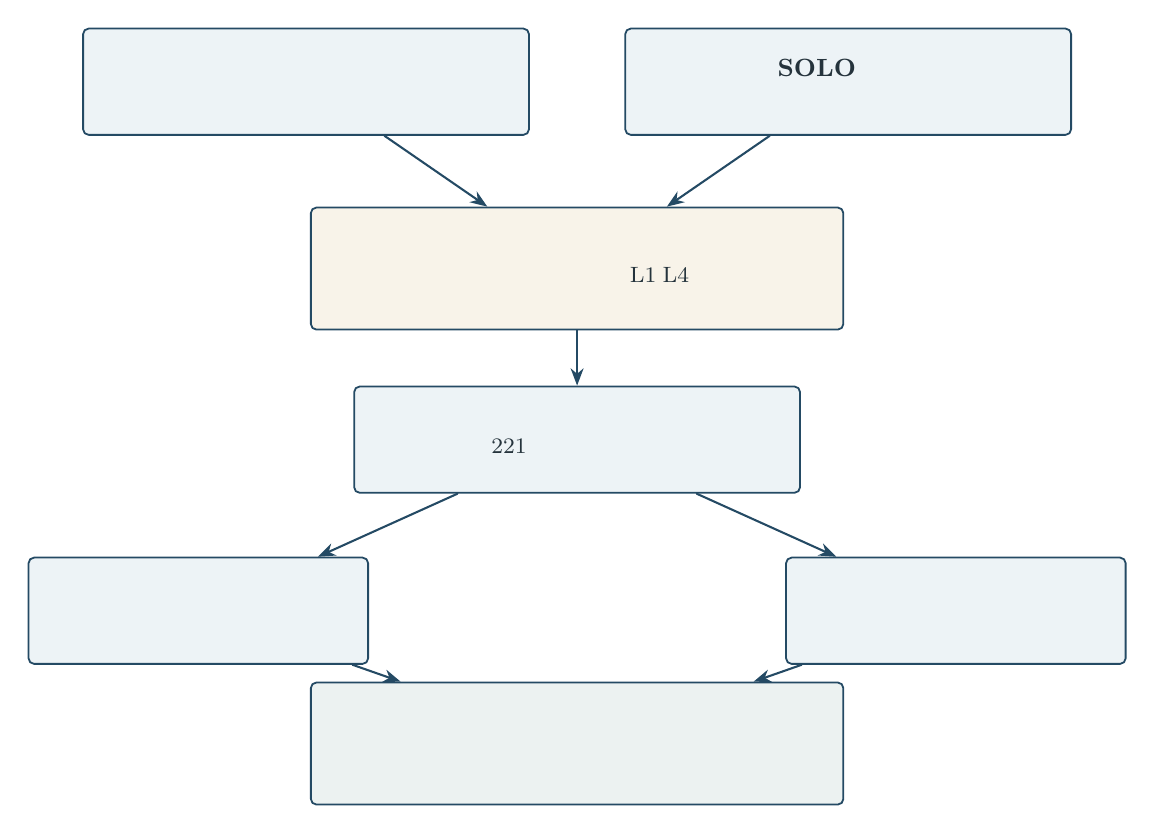
\begin{tikzpicture}[
  node distance=7mm and 12mm,
  every node/.style={font=\small},
  source/.style={thesisbox,text width=5.1cm,minimum height=1.35cm},
  core/.style={thesisbox,text width=6.2cm,minimum height=1.55cm,fill=ThesisGold!12},
  output/.style={thesisbox,text width=3.75cm,minimum height=1.35cm}
]
  \node[source] (science) {\textbf{科学思维的课程与研究表述}\\[-1pt]\footnotesize 模型建构、科学推理、科学论证、质疑创新};
  \node[source,right=of science] (solo) {\textbf{SOLO理论与内容分析方法}\\[-1pt]\footnotesize 任务结构层次、分析单位、判定证据与复核规则};
  \coordinate (source-bottom-mid) at ($(science.south)!0.5!(solo.south)$);
  \node[core,below=9mm of source-bottom-mid] (coding) {\textbf{两层任务编码框架}\\[-1pt]\footnotesize 第一层：维度是否出现\quad 第二层：出现维度的结构等级L1至L4};
  \node[source,below=of coding] (evidence) {\textbf{小问级语料与证据链}\\[-1pt]\footnotesize 221个分析单元；题干、参考解答及相邻等级排除理由};
  \node[output,below left=8mm and -2mm of evidence] (distribution) {\textbf{总体结构}\\[-1pt]\footnotesize 维度分布、等级构成、组合与届次};
  \node[output,below right=8mm and -2mm of evidence] (mechanism) {\textbf{案例机制}\\[-1pt]\footnotesize 条件、模型、关系链、比较与边界};
  \node[core,below=9mm of $(distribution)!0.5!(mechanism)$,fill=ThesisTeal!11] (teaching) {\textbf{教学设计启示}\\[-1pt]\footnotesize 由任务结构形成学习任务、支架、可观察产出与反馈要点};
  \draw[thesisarrow] (science) -- (coding);
  \draw[thesisarrow] (solo) -- (coding);
  \draw[thesisarrow] (coding) -- (evidence);
  \draw[thesisarrow] (evidence) -- (distribution);
  \draw[thesisarrow] (evidence) -- (mechanism);
  \draw[thesisarrow] (distribution) -- (teaching);
  \draw[thesisarrow] (mechanism) -- (teaching);
\end{tikzpicture}
\caption{试题任务认知要求分析的理论框架}
\label{fig:theoretical-framework}
\end{figure}

从图2-1可以看到，理论概念并不直接导出教学结论，而是需要经过操作化、语料编码和案例解释三个环节。课程标准和相关理论提供维度选择的依据，编码手册将抽象概念转化为可判定的规则，描述统计呈现全样本中的任务结构分布，案例分析再把分布中的典型结构还原为具体题设与解答。教学设计建议位于这一链条的末端，其作用是把已经识别的任务结构转化为可实施的学习活动，而不是把统计比例直接转换为教学成效。

这一框架的关键不在于给每道题贴上一个笼统的``高''或``低''标签，而在于将任务中的不同工作分别呈现出来。以一道含有近似条件的力学题为例，学生可能需要先确定系统与研究对象，这是模型建构；再将受力、运动关系与边界条件连成推演链，这是科学推理；若题目要求说明近似何时失效，则还涉及科学论证；若进一步要求改变限制条件并比较新的处理方案，才可能出现质疑创新。四类活动在实际求解中彼此衔接，但它们并不应因最终都写在同一份解答中而被混为一个难度分数。

两层编码还使同一知识内容能够被作出更细的区分。例如，光学题既可以要求在已给几何关系下直接推导，也可以要求比较不同光路、说明近轴近似的适用范围；电磁学题既可以要求调用场与力的关系，也可以要求在不同参数条件下重新选择模型。前者和后者使用的知识点可能相近，却对条件组织、关系整合和结论说明提出不同要求。只有将维度出现与结构等级分开记录，才可能在保持物理内容完整的同时说明这种差异。

从教学设计的角度看，框架提供的不是现成的学生评价等级，而是一种拆解任务的工具。教师可以据此决定一题的评讲重点是补充模型假设、梳理推理链、要求理由说明，还是安排改变条件后的再判断；学生的实际作品则需要另有材料和规则评价。把任务要求与学生表现区分开来，既避免将文本分析误作学习诊断，也使后续课堂研究拥有明确的观察起点。

\section{本章小结}\label{ux672cux7ae0ux5c0fux7ed3-1}

\subsection{本章总结}\label{ux672cux7ae0ux603bux7ed3-1}

本章从科学思维四维度、SOLO启发的任务认知结构要求、两层编码逻辑和案例解释路径四个方面建立分析框架。该框架将研究对象限定为试题任务要求，而不以题目文本替代学生真实能力；将维度存在性与结构等级分开记录，而不以综合总分覆盖不同性质的任务；将总体统计与具体物理案例相互连接，使后续教学设计能够回到可见的题设条件和解答关系。\textsuperscript{[1, 2, 3, 6]}

\chapter{研究设计与编码框架}\label{ux7814ux7a76ux8bbeux8ba1ux4e0eux7f16ux7801ux6846ux67b6}

\section{总体研究设计}\label{ux603bux4f53ux7814ux7a76ux8bbeux8ba1}

\subsection{研究思路与分析对象}\label{ux7814ux7a76ux601dux8defux4e0eux5206ux6790ux5bf9ux8c61}

本研究以第35至42届全国中学生物理竞赛复赛试题为分析对象，采用内容分析的方法，考察复赛试题在模型建构、科学推理、科学论证和质疑创新四个维度上呈现的任务认知要求。研究对象是试题及参考解答对解题者提出的认知活动要求，而非学生实际表现出的科学思维水平。科学推理和科学思维测评研究表明，学生能力判断需要专门测评任务、学生作答数据和模型检验；自由作答研究也以学生书面作答中的可见证据为编码对象。\textsuperscript{[2, 3, 18]}
因此，本文中的等级判断均表述为``试题认知结构要求''或``任务结构复杂性''。

研究已建立第35至42届试题语料库、V3编码手册、逐条题干---解答证据、作者复核记录和唯一编码表。本文将分析结果界定为可追溯的描述性结果，不将其等同于学生能力测量或教学效果证据。

为使研究设计与证据范围相对应，表3-1将本研究的材料层、编码层、分析层和教学设计层分开呈现。各层之间通过明确的输入、输出和限制逐层衔接。

\begin{longtable}[]{@{}
  >{\raggedright\arraybackslash}p{(\linewidth - 8\tabcolsep) * \real{0.2000}}
  >{\raggedright\arraybackslash}p{(\linewidth - 8\tabcolsep) * \real{0.2000}}
  >{\raggedright\arraybackslash}p{(\linewidth - 8\tabcolsep) * \real{0.2000}}
  >{\raggedright\arraybackslash}p{(\linewidth - 8\tabcolsep) * \real{0.2000}}
  >{\raggedright\arraybackslash}p{(\linewidth - 8\tabcolsep) * \real{0.2000}}@{}}
\caption{研究材料、分析产出与解释边界}\tabularnewline
\toprule\noalign{}
\rowcolor{ThesisPale}
\begin{minipage}[b]{\linewidth}\raggedright
层面
\end{minipage} & \begin{minipage}[b]{\linewidth}\raggedright
研究材料
\end{minipage} & \begin{minipage}[b]{\linewidth}\raggedright
分析产出
\end{minipage} & \begin{minipage}[b]{\linewidth}\raggedright
本文用途
\end{minipage} & \begin{minipage}[b]{\linewidth}\raggedright
不作的推断
\end{minipage} \\
\midrule\noalign{}
\endfirsthead
\toprule\noalign{}
\rowcolor{ThesisPale}
\begin{minipage}[b]{\linewidth}\raggedright
层面
\end{minipage} & \begin{minipage}[b]{\linewidth}\raggedright
研究材料
\end{minipage} & \begin{minipage}[b]{\linewidth}\raggedright
分析产出
\end{minipage} & \begin{minipage}[b]{\linewidth}\raggedright
本文用途
\end{minipage} & \begin{minipage}[b]{\linewidth}\raggedright
不作的推断
\end{minipage} \\
\midrule\noalign{}
\endhead
\bottomrule\noalign{}
\endlastfoot
语料层 & 第35至42届复赛题面、参考解答与小问级元数据 &
221个分析单元及其定位入口 & 界定试题材料与分析范围 &
学生样本、学生成绩或命题长期趋势 \\
编码层 & 四维度规则、L1至L4规则、题干---解答证据 & 884条V3编码与判定依据
& 描述任务要求的出现、等级与组合 & 学生真实思维、框架外部效度 \\
分析层 & 编码表与统计程序 & 分布、等级、共现和分组表 &
研究语料的描述统计 & 显著性、因果、跨届普遍规律 \\
教学设计层 & 六个典型案例与任务结构 & 任务、支架、可观察产出和反馈建议 &
教学设计启示 & 学生困难、教师共识或教学效果 \\
\end{longtable}

表3-1的分层也决定了论文的论证顺序：第四章报告分析层结果，第五章将结果转化为教学设计材料。学生、教师或课堂资料属于另一类经验性证据，不能以题目或参考解答编码替代。

\section{语料来源与分析单位}\label{ux8bedux6599ux6765ux6e90ux4e0eux5206ux6790ux5355ux4f4d}

\subsection{语料范围与小问级单位}\label{ux8bedux6599ux8303ux56f4ux4e0eux5c0fux95eeux7ea7ux5355ux4f4d}

本研究语料为第35至42届复赛试题和参考答案PDF，并建立``复赛试题小问级索引表''，共包含221个分析单元。分析单位优先采用独立小问；若同一小问内部包含相对独立的作答目标，则进一步拆分为分析单元。每条记录均保留届次、年份、题号、小问号、试题页码、答案页码、知识模块、情境、表征、数学工具和答案结构等元数据。V3复核期间补入第42届第1题第（4）问和第4题第（3）问两个此前漏列单元，因而当前口径由早期版本的219个单元修正为221个。

相邻的物理教育内容分析研究也表明，分析单位应随研究问题与材料性质明确界定，并公开纳入、排除与样本边界；其以教材图件为单位的规则不能原样迁移到本研究的小问级竞赛任务。\textsuperscript{[19]}

相邻的中国物理考试题内容分析会将同一大题中可相对独立、且要求不同认知操作的任务分别登记，并把题目中的图、表或示意图是否构成任务条件、是否要求生成表征写入纳入规则。因此，本研究拆分复赛大题时，以题干、题图和参考解答能够分别定位为前提；图件只作为支持任务要求的证据之一，不因其形式本身自动触发某一科学思维维度或等级。\textsuperscript{[20]}

相邻的物理试题研究还把数值、公式、文字、概念、图像与由文字触发的视觉化作为可并存的呈现特征登记。其中，图像是否出现与题干是否还要求解题者进行空间想象并非同一判断。因此，本研究只将题图、题表、公式和文字说明作为可定位的任务材料证据；任何单一呈现形式都不自动决定某一科学思维维度或任务结构等级。\textsuperscript{[21]}

相邻的物理题文本分类研究提示，除公布语料范围和分析单位外，还应说明判定依据、示例及分歧处理；题目所要求的认知过程还会受先备知识和相似题经验等分析前提影响。故本研究保留题干---参考解答定位、编码手册版本和分歧裁决记录，并只把它们用于描述试题任务要求，不据此推定参赛者实际采用的策略、能力或学习结果。\textsuperscript{[22, 23]}

另一项中国物理考试文本研究将内容主题与认知要求分开编码，公开样本范围、条目拆分规则、编码示例和二维汇总方式。这提示本研究应交代小问级分析单位、维度判据与汇总过程；但其SEC模型、认知水平定义、高考样本、一致性系数和命题建议均不迁移到本研究的竞赛语料。\textsuperscript{[24]}

语料整理过程中，对OCR文本、公式与特殊符号、题图裁边与图注以及分值资料进行了人工校对。校对结果与题干、参考解答和图件材料相互对应，为后续编码提供了清晰的文本基础。

第35届解答与评分标准记录了26个小问的逐项配分，并把多数得分点落实到编号公式、关键推导或结论；该届8道大题均为40分。由于各届可得配分资料的颗粒度不统一，本文以小问等权作为全样本主分析口径；第35届逐步骤评分资料用于材料完整性核对和单届敏感性检查，不进入跨届加权比较。

\subsection{小问拆分与元数据记录}\label{ux5c0fux95eeux62c6ux5206ux4e0eux5143ux6570ux636eux8bb0ux5f55}

小问级分析的关键不在于将题目机械切碎，而在于保持任务边界与物理意义的一致。对于题干中已经标明的（1）、（2）等子问，通常以子问作为分析单位；若某一子问包含前后相对独立的任务，且后半部分需要重新组织对象、条件或目标量，则将其拆分为相互可定位的分析单元。反之，若若干计算步骤只是围绕同一待求量连续展开，则仍视为一个分析单元。拆分后每个单元均保留与原题号、小问号和页码的对应关系，以保证统计结果能够回到原始题面。

元数据记录服务于后续检索和描述，而不直接作为任务结构等级的替代指标。知识模块用于说明题目涉及的主要物理内容；情境字段记录装置、过程或问题背景；表征字段记录文字、图像、表格、符号等材料形式；数学工具字段记录方程、函数、微积分、几何或其他工具性要素；答案结构字段概括参考解答的主要组织方式。上述字段可以帮助比较不同材料条件下的编码分布，也可以支持案例抽取，但不应据此直接断言某一知识模块或表征形式必然导致更高或更低的科学思维要求。

为降低拆分和元数据记录带来的任意性，研究记录同时保存题面页、答案页、题图或表格定位以及相应的文字说明。这样，当某一统计数字或案例解释需要复查时，可以先定位到分析单元，再回到题干、参考解答和图件材料，而不是只依据汇总表进行二次解释。小问级索引由此构成语料层与编码层之间的连接点。

\section{编码手册开发}\label{ux7f16ux7801ux624bux518cux5f00ux53d1}

\subsection{编码维度与判定规则}\label{ux7f16ux7801ux7ef4ux5ea6ux4e0eux5224ux5b9aux89c4ux5219}

编码框架以科学思维四维度为主体，并引入SOLO理论作为``任务认知结构要求''等级划分的启发来源。编码手册规定每个维度分别判断``是否出现''和``出现时的等级''，避免把计算复杂度、背景陌生度或参考解答篇幅直接等同于高阶思维要求。

四个维度的操作性边界如下。模型建构关注研究对象、系统边界、变量、理想化假设和模型形成；科学推理关注由条件到结论的物理关系链；科学论证关注比较、检验、边界分析和假设辩护；质疑创新仅在题目明确要求处理假设、替代模型、模型失效、开放方案或证据约束的新方案时触发。等级从L1至L4表示任务结构复杂性递增，但不表示学生真实学习结果等级。

存在性判断采用必要活动规则。科学推理只有在完成小问必须把题设条件、中间结果与至少一个具有物理意义的关系连接起来时才出现；仅辨认、直接读取给定量、抄写题设公式或与物理判断无关的机械代数不计入。L1也不是``凡有计算即出现''，而是一个核心物理关系确实承担了由条件到结论的推断功能。模型建构只有在对象、边界、变量、近似或模型选择需要由解题者组织时才出现；模型已完整给定、只在既定关系内推进的任务不自动计入。科学论证和质疑创新分别以``理由或边界是否需要被说明''和``假设或方案是否需要被改变''为核心，不能由``讨论''\,``新颖''等表面措辞替代。

编码手册经历早期试编码、文件比较、高风险边界筛查和V3全量重编码。早期材料用于发现``复杂计算自动升级''\,``整题标签复制''和``把新颖情境视为质疑创新''等边界问题；V3手册据此提高存在性门槛，并要求每条记录写明题干证据、解答证据和相邻等级排除理由。早期版本不参与第四章正式统计。

编码时先判断某维度是否出现，再对``出现''的记录判定L1至L4；若未出现，则等级固定为``未出现''。每条记录均要求保留题干触发语、题面定位、解答关键步骤、答案定位和相邻等级排除说明。这样的记录结构使``存在性判断''\,``等级判断''和``证据定位''能够分别审阅，避免用一个笼统的难度标签覆盖不同性质的判断。

\section{编码框架的审阅与修订}\label{ux7f16ux7801ux6846ux67b6ux7684ux5ba1ux9605ux4e0eux4feeux8ba2}

\subsection{框架审阅与修订}\label{ux6846ux67b6ux5ba1ux9605ux4e0eux4feeux8ba2}

编码框架在试编码、边界案例复查和V3全量重编码过程中持续修订。审阅重点包括四个维度的操作性定义、存在性判据、相邻等级边界，以及题干与参考解答证据能否支持判定。每次修订均保留受影响的记录、修改理由和版本对应关系，最终形成用于正式统计的V3编码手册与唯一编码表。本文未将这一修订过程表述为外部效度检验；框架的跨研究者适用性仍需由身份、训练和互盲过程可核验的独立编码研究进一步检验。

\section{从早期编码到V3全量复核}\label{ux4eceux65e9ux671fux7f16ux7801ux5230v3ux5168ux91cfux590dux6838}

\subsection{早期编码的诊断作用}\label{ux65e9ux671fux7f16ux7801ux7684ux8bcaux65adux4f5cux7528}

研究早期按219个分析单元形成876条V2记录，并对两份匿名回填进行文件比较和分歧处理。该阶段的作用是暴露编码边界：同一大题的多个小问容易被复制为相同标签，计算步骤多容易被误判为高等级，题材新颖也容易被误判为质疑创新。由于回填身份和提交前互盲过程没有独立的现场记录，该阶段结果只作为框架修订材料，不作为V3正式统计来源，也不作为编码框架已经获得外部信度或效度验证的证据。

高风险筛查进一步发现，问题同时涉及维度存在性、等级判定和分析单位完整性，不能通过局部修正恢复旧统计。因此，研究重新编制V3编码手册，对第35至42届全部分析单元进行全量重编码。V3特别强化三项规则：题目背景复杂不自动触发高等级，答案篇幅和公式数量不替代任务结构判断，质疑创新必须有改变假设、比较替代方案、修正模型或开放设计等明确任务。

\subsection{V3作者实质复核}\label{v3ux4f5cux8005ux5b9eux8d28ux590dux6838}

V3重编码首先形成221个分析单元、884条候选记录。每条候选记录均包含维度存在性、等级、题干引文、参考解答引文、证据位置和相邻等级排除理由。作者以R01为复核代号逐题核对题干、参考解答和必要认知活动：337条与既有人工复核标签相同的记录在确认适用范围后迁移，另对547条标签变化或新增记录分四批完成实质复核。

复核结果为869条保持V3候选、15条更正、0条待核实。15条更正均保存原候选、复核决定和具体理由；四批文件合并后再次检查884个``分析单元---维度''复合键、字段完整性、题目源文件哈希和题干---解答双侧证据。通过总验收后，生成一份V3唯一编码表，作为第四章统计和第五章案例标签的唯一来源。

这种复核程序提高了判定过程的可追溯性，但其证据性质仍须准确表述：V3结果是经过作者全量实质复核的内容分析结果，不是由可核验互盲程序产生的独立评分者一致性研究。后续研究仍可邀请独立编码者依据同一手册重新编码，以检验规则在不同研究者之间的适用性。

\section{正式编码与数据处理}\label{ux6b63ux5f0fux7f16ux7801ux4e0eux6570ux636eux5904ux7406}

\subsection{编码流程与统计处理}\label{ux7f16ux7801ux6d41ux7a0bux4e0eux7edfux8ba1ux5904ux7406}

正式数据处理依次包括分析单位核对、V3候选编码、作者逐题复核、候选更正、字段与证据校验、唯一表生成和描述统计输出。对于引文不足、题干与解答对应不清或边界较为复杂的记录，研究回到原题和参考解答后再作判断。最终形成221个分析单元、884条唯一编码记录，并据此生成总体出现、等级构成、维度组合、两两共现和分届次描述表。

语料索引还保留知识模块、题面表征、数学工具和答案结构等小问级元数据。这些字段用于回查题目和选择案例，不直接参与V3等级计算。由于具体题材表述尚未经过统一分类规则复核，第四章不再沿用早期版本的知识模块、表征要素数或数学工具要素数分组统计，以免把机械计数误作认知复杂性指标。

正式描述统计采用作者复核并通过总验收的V3唯一编码表。该表的版本校验值为
\texttt{c026c2c48a6ff97987896261b1a3403b35e91c9e619e352809812c0e4095c8d5}。第四章、摘要、结论和案例标签均由该版本统一生成或逐项核对；早期V2结果只保留在版本档案中，不参与当前结果报告。

为保证数据版本一致，处理程序检验编码表中884个``分析单元---维度''复合键的唯一性，确认每个分析单元恰有四条维度记录，再由同一编码表生成七张中文统计表和四幅正式图件。语料索引、编码表、统计输出和图件同时保存版本标识或校验值，用于识别不同版本之间的错配。上述措施保证统计结果能够回溯到相应记录，但不替代对编码规则和物理解释的独立审查。

\subsection{描述统计与结果解释}\label{ux63cfux8ff0ux7edfux8ba1ux4e0eux7ed3ux679cux89e3ux91ca}

本研究以分析单元等权作为全样本的基本统计口径。对于每个维度，首先统计被判定为``出现''的分析单元数及其占221个分析单元的比例；对于等级分布，则以该维度已经出现的单元数为分母，分别呈现L1至L4的构成。由于同一小问可以同时包含多个科学思维维度，四个维度的出现数不相互排斥，也不相加构成所谓``总思维分''。

维度组合统计记录每个分析单元实际出现的完整维度组合；两两共现统计报告交集、并集和Jaccard系数，用于展示集合重叠程度。Jaccard系数不能替代相关系数、效应量或因果指标。分届次统计用于呈现八届样本内部的描述背景，为案例阅读提供定位，不检验跨届趋势或组间显著性差异。

结果解释遵循``统计表---题干与解答---案例材料''的顺序。统计表回答总体上出现了什么，题干与参考解答说明某一判定在何种任务结构中产生，案例分析则将这些结构转换为可讨论的教学任务。通过这一顺序，描述性统计既保持全样本视野，也避免将抽象比例脱离具体物理情境进行解释。

这一统计口径特别重视分母的可解释性。维度出现比例以221个分析单元为共同分母，回答某类任务要求在全部小问中出现的范围；等级构成则以相应维度已经出现的单元为分母，回答该类任务内部的结构分布。二者不能混用。例如，科学论证的等级构成只应在36个已出现科学论证的单元中理解，不能把其L1、L2、L3直接与其他维度作``高低''比较。将分母写清楚，是避免统计表被误读为学生能力比例或总难度分布的基本条件。

共现分析也遵循同样的克制原则。若模型建构与科学推理在同一单元中共同出现，所能说明的是该单元的完成同时需要组织模型与推演关系；它不能证明两个维度在心理机制上必然相关，更不能说明学生掌握其中一个维度后必然掌握另一个维度。Jaccard系数用于展示两个集合的重叠程度，其解释仍须回到具体题目中条件、模型和推导的组织方式。因而，本研究把共现表视为案例检索工具，而不是对变量关系进行因果解释的证据。

对于届次描述，本文采用``先报告样本、后核对材料''的阅读原则。某一届次的比例若值得讨论，首先检查该届分析单元数和小问拆分方式，再回到题干和解答确认具体任务机制。八届数据不是经过时间序列设计得到的观测，因此正文不把届次波动解释为命题趋势。

第四章报告基于试题文本的描述性结果；第五章据此提出教学设计建议。两章的论证对象分别是试题任务分布和由任务结构形成的设计方案。

\section{教学设计启示的形成方法}\label{ux6559ux5b66ux8bbeux8ba1ux542fux793aux7684ux5f62ux6210ux65b9ux6cd5}

\subsection{从任务结构到教学设计}\label{ux4eceux4efbux52a1ux7ed3ux6784ux5230ux6559ux5b66ux8bbeux8ba1}

教学设计部分采用``任务结构---学习任务---支架---可观察产出---反馈要点''的链条。任务结构来自题干与参考解答中反复出现的条件组织、关系连接、状态分类、近似处理、对象比较和阈值判断；学习任务规定学生实际要完成的工作；支架帮助学生进入任务；可观察产出为教师检查提供材料；反馈要点则回到条件、模型、关系与结论边界。科学论证教学研究和国际科学实践框架为任务、支架和评价对象提供设计参照。\textsuperscript{[4, 5]}

六个典型案例分别对应条件---关系链、状态分类与比较、近似条件建模、同对象比较、多对象约束和阈值判断。每项建议均给出可观察的学习产出，例如条件表、关系图、状态分支、近似说明、对象---约束表或临界判断图，使教学启示能够落实为可布置、可提交和可反馈的活动。

\section{伦理与质量控制}\label{ux4f26ux7406ux4e0eux8d28ux91cfux63a7ux5236}

\subsection{研究质量控制}\label{ux7814ux7a76ux8d28ux91cfux63a7ux5236}

本研究使用公开发布或作者取得的竞赛试题与参考答案，不涉及学生个人数据。本文未使用教师访谈、问卷、学生作答或课堂观察资料。未来若扩展至参与者研究，应另行履行知情同意、匿名化、数据保存和伦理审查程序，并将参与者资料与试题分析数据分开管理。

质量控制包括四个层面。第一，语料层面保留原始PDF、题干文本、题图资产和校对记录；第二，框架层面保留V3编码手册、判定规则和边界案例；第三，编码层面保留候选记录、作者逐题复核、15条更正和总验收记录；第四，分析层面以同一唯一编码表生成统计表和图件，并通过独立程序复算，避免手工计算造成版本错配。

\subsection{语料与文本质量控制}\label{ux8bedux6599ux4e0eux6587ux672cux8d28ux91cfux63a7ux5236}

语料质量控制首先关注材料边界是否清楚。每份试题和参考答案均以届次、题号、页码和文件校验信息登记，题干与解答文本分别保留，以避免将题目要求与参考答案步骤混为同一材料。对于公式、特殊符号、图件裁边或答案页边界等容易影响理解的内容，研究记录保留相应的校对入口和定位信息。这样做的目的不是把文本处理过程写成研究发现，而是保证后续编码能够回到足以判断任务要求的材料。

第二，文本质量控制关注分析单位与原始材料之间的对应。每个分析单元都保留其所属大题、小问、题面页和答案页，使小问拆分不会脱离原题语境。若一个统计结果或案例解释涉及图像、公式或条件限制，读者可以沿索引回查相应材料。对内容分析而言，这种可回查性比单纯扩大样本数量更重要，因为它使研究者能够发现并修正拆分、转写或定位中的问题。

\subsection{编码与分析质量控制}\label{ux7f16ux7801ux4e0eux5206ux6790ux8d28ux91cfux63a7ux5236}

编码质量控制强调规则、证据和版本之间的一致。编码手册明确维度定义、等级含义、排除规则和边界情形；每条编码记录同时保存题干触发语和解答关键步骤；出现分歧时，先回到材料和规则，而不是只根据统计结果调整判断。这样的流程使``为什么这样编码''能够得到具体回答，也使后续修订能够定位受影响的单元与维度。

分析质量控制则避免正文数字与输入数据脱节。总体分布、等级分布、维度共现和分层表均由当前编码表重新计算，图件、表格和案例选择与同一版本的结果保持对应。当编码值发生更正时，需要同步检查描述统计、图件和正文解释是否仍然一致。可复现并不意味着研究结论永远不变，而是意味着结论变化时能够清楚说明变化来自哪一条规则、哪一份材料或哪一项编码修订。

在论文写作中，质量控制还表现为主张强度与证据类型相匹配。题干和参考解答可以支持对任务要求的描述，编码和统计可以支持对当前语料分布的概括，教学设计材料可以支持对任务、支架和评价方式的建议；这些材料不能替代学生作答、教师访谈或课堂实施数据。将不同证据类型分层处理，有助于保持论文结论的准确性，也为后续研究提供明确的扩展方向。

\section{本章小结}\label{ux672cux7ae0ux5c0fux7ed3-2}

\subsection{本章总结}\label{ux672cux7ae0ux603bux7ed3-2}

本章说明了研究设计、语料来源、分析单位、V3编码框架、作者实质复核流程和质量控制方案。下一章将基于221个分析单元、884条V3唯一编码记录，报告复赛试题科学思维要求的描述性结果。

本文不将试题编码结果推断为学生能力、教学效果、因果关系、显著性差异或长期命题趋势。若编码规则或具体判断发生修订，应同步检查统计输出、表格、图件和正文解释。

\chapter{科学思维要求的描述性分析}\label{ux79d1ux5b66ux601dux7ef4ux8981ux6c42ux7684ux63cfux8ff0ux6027ux5206ux6790}

\section{数据基础与统计口径}\label{ux6570ux636eux57faux7840ux4e0eux7edfux8ba1ux53e3ux5f84}

\subsection{正式分析数据}\label{ux6b63ux5f0fux5206ux6790ux6570ux636e}

本章以第35至42届复赛理论试题的221个分析单元为对象。每个分析单元分别记录模型建构、科学推理、科学论证和质疑创新四个维度，共形成884条V3唯一编码记录。该版本已经完成作者逐题实质复核、复合键检查、证据字段检查和统计结果独立复算，是本章全部表格、图件和比例的共同数据源。

统计采用分析单元等权口径。维度出现比例以221个分析单元为分母；等级构成只在该维度已经出现的单元中计算；完整组合记录同一单元实际出现的维度集合；两两共现记录交集、并集和Jaccard系数。所有结果均描述试题及参考解答呈现的任务要求，不代表学生实际能力、作答表现或教学效果。

\subsection{结果解释原则}\label{ux7ed3ux679cux89e3ux91caux539fux5219}

本章的解释依次回答三个问题：某类任务要求在样本中出现多广，出现后主要呈现何种结构等级，不同维度在同一小问中如何组合。届次表用于显示八届语料的内部构成，不能直接用于判断命题趋势。科学推理的出现率达到100\%，意味着该二元指标在本样本中没有变异，因此其区分信息应从L1至L3等级和具体物理关系结构中寻找。

\section{四维度出现分布}\label{ux56dbux7ef4ux5ea6ux51faux73b0ux5206ux5e03}

\subsection{总体出现比例}\label{ux603bux4f53ux51faux73b0ux6bd4ux4f8b}

表4-1和图4-1呈现四个维度在221个分析单元中的出现情况。

\begin{table}[H]
\centering
\caption{四维度在全部分析单元中的出现分布}
\label{tab:v3-overall-presence}
\begin{tabular}{lrrr}
\toprule
维度 & 出现单元数 & 全部单元数 & 出现比例 \\
\midrule
模型建构 & 202 & 221 & 91.40\% \\
科学推理 & 221 & 221 & 100.00\% \\
科学论证 & 36 & 221 & 16.29\% \\
质疑创新 & 2 & 221 & 0.90\% \\
\bottomrule
\end{tabular}
\end{table}

\begin{figure}[H]
\centering
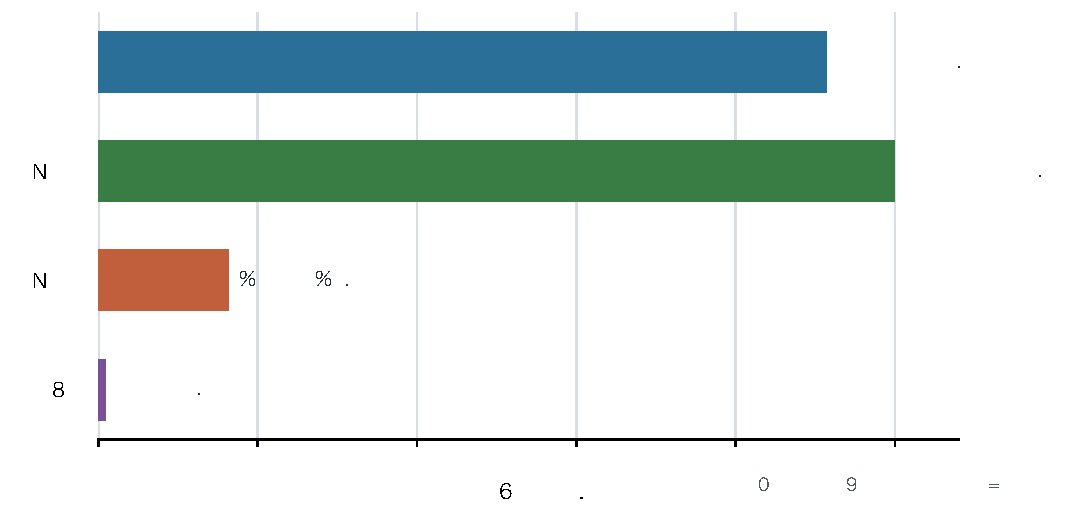
\includegraphics[width=0.86\linewidth]{08_manuscript/figures/v3_final/图4-1_四维度出现比例_V3.pdf}
\caption{四维度在221个分析单元中的出现比例}
\label{fig:v3-overall-presence}
\end{figure}

科学推理出现于全部221个分析单元。按V3规则，这表示每个独立作答目标都要求解题者在题设条件、中间结果与物理关系之间建立至少一条必要联系。该结果不是把``有计算''等同于科学推理，而是逐题核对必要认知活动后的编码结果。由于出现率已经饱和，它不能用来区分届次，也不能说明所有小问的推理结构相同。

模型建构出现于202个单元，占91.40\%。这说明大多数小问除关系推演外，还要求组织研究对象、变量、边界、理想化条件或模型表达；另有19个单元在模型已由题面或前问充分给定的情况下继续推进，未重复计入模型建构。科学论证只出现于36个单元，主要对应题面明确要求证明、比较、检验或说明适用边界的任务。质疑创新仅出现2次，反映V3规则对该维度采用较严格的进入门槛：陌生情境、复杂运算或已有方案的直接应用均不能单独触发质疑创新。

\section{四维度等级构成}\label{ux56dbux7ef4ux5ea6ux7b49ux7ea7ux6784ux6210}

\subsection{出现单元内部的等级分布}\label{ux51faux73b0ux5355ux5143ux5185ux90e8ux7684ux7b49ux7ea7ux5206ux5e03}

等级分布的分母是各维度已经出现的单元数，而不是统一的221。表4-2同时给出频数和维度内比例。

\begin{longtable}[]{@{}lrrrrr@{}}
\caption{四维度出现单元内部的等级构成}\tabularnewline
\toprule\noalign{}
\rowcolor{ThesisPale}
维度 & 出现单元数 & L1 & L2 & L3 & L4 \\
\midrule\noalign{}
\endfirsthead
\toprule\noalign{}
\rowcolor{ThesisPale}
维度 & 出现单元数 & L1 & L2 & L3 & L4 \\
\midrule\noalign{}
\endhead
\bottomrule\noalign{}
\endlastfoot
模型建构 & 202 & 9（4.46\%） & 77（38.12\%） & 116（57.43\%） & 0 \\
科学推理 & 221 & 13（5.88\%） & 69（31.22\%） & 139（62.90\%） & 0 \\
科学论证 & 36 & 14（38.89\%） & 16（44.44\%） & 6（16.67\%） & 0 \\
质疑创新 & 2 & 0 & 2（100.00\%） & 0 & 0 \\
\end{longtable}

\begin{figure}[H]
\centering
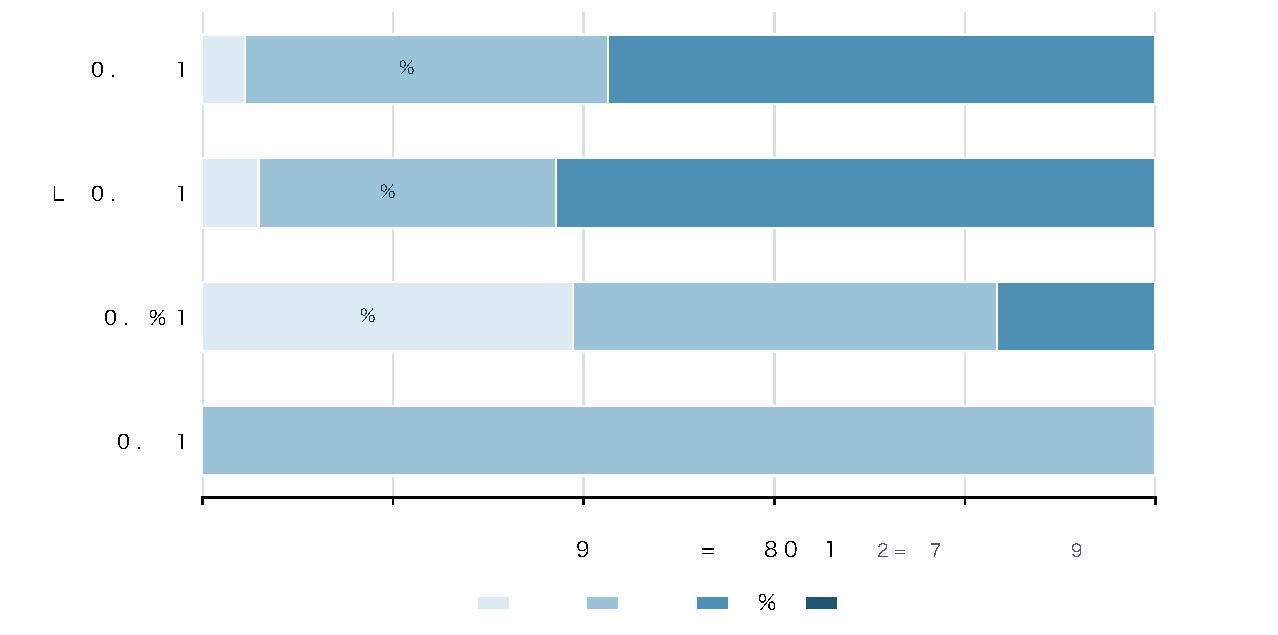
\includegraphics[width=0.88\linewidth]{08_manuscript/figures/v3_final/图4-2_四维度等级构成_V3.pdf}
\caption{四维度出现单元内部的等级构成}
\label{fig:v3-level-composition}
\end{figure}

模型建构和科学推理均以L3为主，分别为116个和139个单元。这些单元的共同特征不是公式数量多，而是完成任务需要协调多个模型要素、条件或物理关系。L2模型建构和科学推理分别为77个和69个单元，主要表现为在两个相互联系的要素或关系之间完成组织；L1数量较少，分别为9个和13个单元，对应单一模型要素或核心关系承担主要任务的情形。

科学论证的36个出现单元中，L2有16个，L1有14个，L3有6个。其内部结构比总体出现率更能说明论证任务的差异：有的小问只要求针对一个结论给出直接理由，有的需要组织多项依据或比较条件，少数任务还要求对多层条件、边界或相互竞争的结论作较完整说明。质疑创新仅有2个L2单元，样本过少，不宜据此概括稳定的等级结构。

四个维度均未出现L4。该结果只表示在V3操作性定义下，没有分析单元同时满足相应维度的L4最低充分条件；它不意味着复赛试题整体缺乏挑战，也不意味着学生不能表现出更复杂的思维。任务结构等级与经验难度、得分难度和学生能力属于不同判断。

\section{维度组合与共现结构}\label{ux7ef4ux5ea6ux7ec4ux5408ux4e0eux5171ux73b0ux7ed3ux6784}

\subsection{完整维度组合}\label{ux5b8cux6574ux7ef4ux5ea6ux7ec4ux5408}

221个分析单元共形成五种完整组合，见表4-3和图4-3。

\begin{longtable}[]{@{}lrr@{}}
\caption{五种完整维度组合的分布}\tabularnewline
\toprule\noalign{}
\rowcolor{ThesisPale}
完整维度组合 & 单元数 & 占全部单元比例 \\
\midrule\noalign{}
\endfirsthead
\toprule\noalign{}
\rowcolor{ThesisPale}
完整维度组合 & 单元数 & 占全部单元比例 \\
\midrule\noalign{}
\endhead
\bottomrule\noalign{}
\endlastfoot
模型建构＋科学推理 & 168 & 76.02\% \\
模型建构＋科学推理＋科学论证 & 32 & 14.48\% \\
仅科学推理 & 17 & 7.69\% \\
模型建构＋科学推理＋科学论证＋质疑创新 & 2 & 0.90\% \\
科学推理＋科学论证 & 2 & 0.90\% \\
\end{longtable}

\begin{figure}[H]
\centering
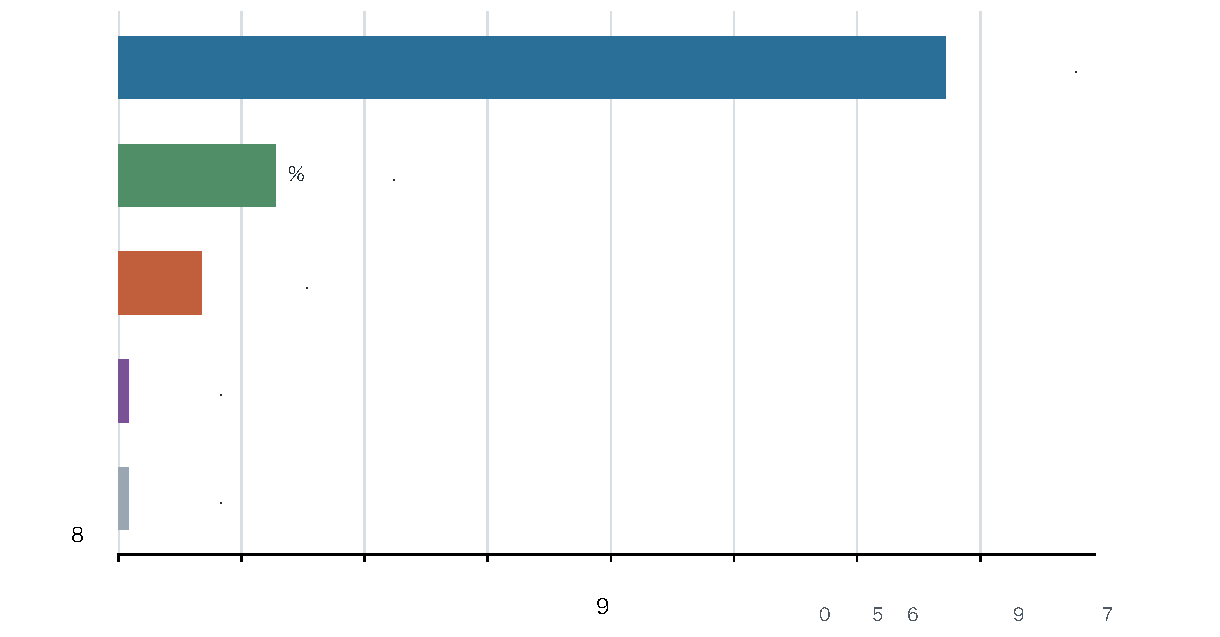
\includegraphics[width=0.88\linewidth]{08_manuscript/figures/v3_final/图4-4_维度组合分布_V3.pdf}
\caption{221个分析单元的完整维度组合分布}
\label{fig:v3-combination}
\end{figure}

``模型建构＋科学推理''是最主要的组合，共168个单元，占76.02\%。这类小问要求解题者组织对象、条件或模型，并在此基础上完成关系推演，但题面没有提出独立的论证或方案改变任务。另有32个单元在建模和推理之外明确要求科学论证，占14.48\%。仅科学推理的17个单元通常在模型和必要条件已经给定的情况下，直接完成关系调用或局部推演。

四维同时出现仅有2个单元。这两个单元同时满足模型组织、关系推演、理由说明和方案或假设调整的进入条件，但数量不足以代表复赛试题的普遍结构。完整组合的分布还表明，质疑创新没有单独出现，也没有与部分维度形成其他组合；这一现象来自当前两个具体单元，不能据此推导维度之间的理论从属关系。

\subsection{两两共现}\label{ux4e24ux4e24ux5171ux73b0}

表4-4列出六组维度对的交集、并集和Jaccard系数。

\begin{longtable}[]{@{}lrrr@{}}
\caption{四维度的两两共现分布}\tabularnewline
\toprule\noalign{}
\rowcolor{ThesisPale}
维度对 & 共同出现单元数 & 至少一维出现单元数 & Jaccard系数 \\
\midrule\noalign{}
\endfirsthead
\toprule\noalign{}
\rowcolor{ThesisPale}
维度对 & 共同出现单元数 & 至少一维出现单元数 & Jaccard系数 \\
\midrule\noalign{}
\endhead
\bottomrule\noalign{}
\endlastfoot
模型建构---科学推理 & 202 & 221 & 0.9140 \\
模型建构---科学论证 & 34 & 204 & 0.1667 \\
模型建构---质疑创新 & 2 & 202 & 0.0099 \\
科学推理---科学论证 & 36 & 221 & 0.1629 \\
科学推理---质疑创新 & 2 & 221 & 0.0090 \\
科学论证---质疑创新 & 2 & 36 & 0.0556 \\
\end{longtable}

模型建构与科学推理共同出现202次，是因为全部模型建构单元同时包含必要的关系推演。科学论证与模型建构共同出现34次，另有2个科学论证单元未重复计入模型建构；它们在题面已经给定模型的情况下，要求继续推理并说明结论。质疑创新的两次出现均与其他三维同时发生。表中的Jaccard系数只用于描述集合重叠，不是相关系数，更不能解释为一个维度导致另一个维度。

\section{分届次描述}\label{ux5206ux5c4aux6b21ux63cfux8ff0}

\subsection{各届样本与维度出现比例}\label{ux5404ux5c4aux6837ux672cux4e0eux7ef4ux5ea6ux51faux73b0ux6bd4ux4f8b}

八届试题的分析单元数介于22至36之间。表4-5和图4-4呈现各届四维度的出现比例。

\begin{longtable}[]{@{}
  >{\raggedright\arraybackslash}p{(\linewidth - 10\tabcolsep) * \real{0.1304}}
  >{\raggedleft\arraybackslash}p{(\linewidth - 10\tabcolsep) * \real{0.1739}}
  >{\raggedleft\arraybackslash}p{(\linewidth - 10\tabcolsep) * \real{0.1739}}
  >{\raggedleft\arraybackslash}p{(\linewidth - 10\tabcolsep) * \real{0.1739}}
  >{\raggedleft\arraybackslash}p{(\linewidth - 10\tabcolsep) * \real{0.1739}}
  >{\raggedleft\arraybackslash}p{(\linewidth - 10\tabcolsep) * \real{0.1739}}@{}}
\caption{第35至42届四维度出现分布}\tabularnewline
\toprule\noalign{}
\rowcolor{ThesisPale}
\begin{minipage}[b]{\linewidth}\raggedright
届次（年份）
\end{minipage} & \begin{minipage}[b]{\linewidth}\raggedleft
分析单元数
\end{minipage} & \begin{minipage}[b]{\linewidth}\raggedleft
模型建构
\end{minipage} & \begin{minipage}[b]{\linewidth}\raggedleft
科学推理
\end{minipage} & \begin{minipage}[b]{\linewidth}\raggedleft
科学论证
\end{minipage} & \begin{minipage}[b]{\linewidth}\raggedleft
质疑创新
\end{minipage} \\
\midrule\noalign{}
\endfirsthead
\toprule\noalign{}
\rowcolor{ThesisPale}
\begin{minipage}[b]{\linewidth}\raggedright
届次（年份）
\end{minipage} & \begin{minipage}[b]{\linewidth}\raggedleft
分析单元数
\end{minipage} & \begin{minipage}[b]{\linewidth}\raggedleft
模型建构
\end{minipage} & \begin{minipage}[b]{\linewidth}\raggedleft
科学推理
\end{minipage} & \begin{minipage}[b]{\linewidth}\raggedleft
科学论证
\end{minipage} & \begin{minipage}[b]{\linewidth}\raggedleft
质疑创新
\end{minipage} \\
\midrule\noalign{}
\endhead
\bottomrule\noalign{}
\endlastfoot
第35届（2018） & 26 & 25（96.15\%） & 26（100.00\%） & 3（11.54\%） &
1（3.85\%） \\
第36届（2019） & 22 & 21（95.45\%） & 22（100.00\%） & 0（0.00\%） &
0（0.00\%） \\
第37届（2020） & 22 & 20（90.91\%） & 22（100.00\%） & 6（27.27\%） &
0（0.00\%） \\
第38届（2021） & 25 & 23（92.00\%） & 25（100.00\%） & 2（8.00\%） &
0（0.00\%） \\
第39届（2022） & 27 & 25（92.59\%） & 27（100.00\%） & 4（14.81\%） &
0（0.00\%） \\
第40届（2023） & 36 & 34（94.44\%） & 36（100.00\%） & 6（16.67\%） &
0（0.00\%） \\
第41届（2024） & 32 & 28（87.50\%） & 32（100.00\%） & 10（31.25\%） &
0（0.00\%） \\
第42届（2025） & 31 & 26（83.87\%） & 31（100.00\%） & 5（16.13\%） &
1（3.23\%） \\
\end{longtable}

\begin{figure}[H]
\centering
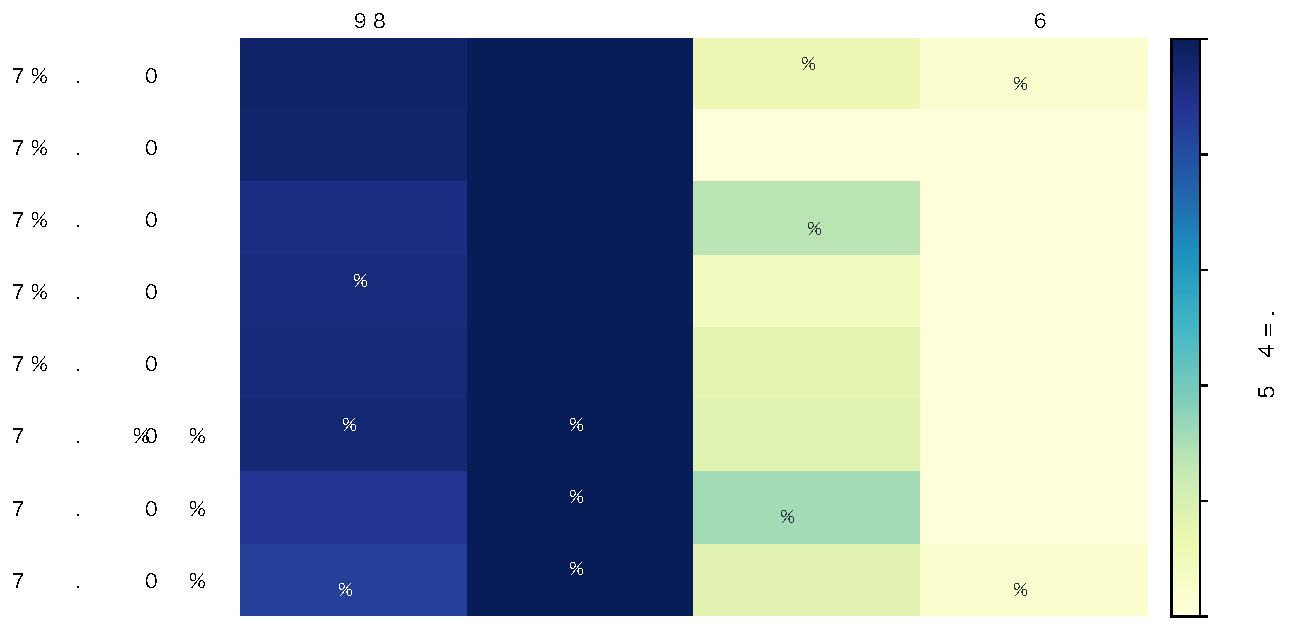
\includegraphics[width=0.94\linewidth]{08_manuscript/figures/v3_final/图4-3_各届次维度出现比例_V3.pdf}
\caption{第35至42届四维度出现比例}
\label{fig:v3-edition-presence}
\end{figure}

科学推理在八届中均为100\%，因此届次层面同样没有二元区分度。模型建构在各届的出现比例为83.87\%至96.15\%，说明各届大多数小问都包含模型组织要求，同时仍保留少量在既定模型内继续推演的单元。科学论证在各届为0至31.25\%，其波动与具体题目是否提出证明、比较、检验或边界说明有关，应回到相应题目解释。质疑创新只在第35届和第42届各出现1次，其他六届均未出现。

这些届次差异是样本内部描述。各届分析单元数量、题材配置和小问结构不同，八个观测点也没有构成时间序列研究设计，因此本文不把比例起伏解释为逐年上升、下降或命题方向变化。届次表的主要用途是帮助定位后续案例：需要阅读论证任务时，可优先回查科学论证出现单元；需要理解严格的质疑创新门槛时，则应直接核对两个正例及其证据。

\section{结果综合}\label{ux7ed3ux679cux7efcux5408}

\subsection{科学思维任务结构的总体特征}\label{ux79d1ux5b66ux601dux7ef4ux4efbux52a1ux7ed3ux6784ux7684ux603bux4f53ux7279ux5f81}

V3结果呈现出清楚的层次。第一，关系推演是全部小问的共同要求，模型组织也覆盖九成以上单元，二者构成复赛任务最稳定的结构基础。第二，模型建构和科学推理在出现单元中均以L3为主，说明多数相关小问需要协调多个条件、模型要素或物理关系，而不只是调用单一公式。第三，科学论证只在有独立证明、比较、检验或边界说明要求时出现；质疑创新的门槛更高，只保留2个明确要求改变假设、方案或模型处理方式的单元。第四，四维同时出现并不是复赛小问的常态，最常见的仍是模型建构与科学推理的组合。

这一结果也说明，不能用一个总分概括复赛试题的科学思维要求。模型组织、关系推演、理由说明和方案调整回答的是不同问题，同一小问可以组合其中若干维度，也可以在某一维度达到较高结构等级而不触发另一维度。第五章因此不把案例简单标成``高阶题''，而是回到具体题干、公式、图示和参考解答，说明各维度如何由物理任务产生。

\subsection{本章小结}\label{ux672cux7ae0ux5c0fux7ed3-3}

本章基于221个分析单元、884条V3唯一编码记录，报告了四维度出现、等级构成、完整组合、两两共现和分届次分布。模型建构、科学推理、科学论证和质疑创新分别出现202、221、36和2次；模型建构与科学推理以L3为主，科学论证以L2略多，质疑创新仅有2个L2单元，四维均未出现L4。最常见组合为模型建构与科学推理，共168个单元。上述统计为第五章选择和解释典型案例提供总体位置，但不替代对具体物理过程的分析。

\chapter{典型案例分析与教学设计启示}\label{ux5178ux578bux6848ux4f8bux5206ux6790ux4e0eux6559ux5b66ux8bbeux8ba1ux542fux793a}

本章选取六个具有代表性的复赛小问，分析题设条件、参考解答与科学思维要求之间的关系，并据此提出教学任务设计建议。案例分析的重点不在于复述完整解答，而在于识别解题过程中的关键转折：条件如何决定模型，模型如何引出关系链，结论又如何通过比较、检验或边界说明获得物理意义。

\section{案例选择与边界}\label{ux6848ux4f8bux9009ux62e9ux4e0eux8fb9ux754c}

\subsection{案例选择原则}\label{ux6848ux4f8bux9009ux62e9ux539fux5219}

案例从已完成编码的复赛小问中选择。入选小问须具有清楚的题面、参考解答和四维度记录，且能够呈现不同的物理任务结构。案例的作用是把第四章的统计结论还原到真实题目中：读者先看到题目要求和关键图示，再理解它为什么被判定为相应的任务结构。案例用于解释试题任务要求和提出教学设计，不用来推断学生表现或教学效果。

\begin{table}[H]
\centering
\caption{典型案例及其任务结构}
\label{tab:v3-case-selection}
\footnotesize
\setlength{\tabcolsep}{3pt}
\renewcommand{\arraystretch}{1.05}
\begin{tabular}{p{2.6cm}p{3.5cm}p{4.5cm}p{2.7cm}}
\toprule
案例 & 任务主题 & V3标签 & 可用于说明的任务结构 \\
\midrule
第41届第6题第（3）问 & 太阳引力场中的飞行方向偏转 & 模型L3、推理L3 & 条件—关系链 \\
第41届第7题第（4）问 & 量子环系统的平均能量 & 模型L3、推理L3、论证L2 & 状态分类—比较 \\
第42届第4题第（2）问 & 强激光场中的相对论电子加速 & 模型L3、推理L3 & 近似条件建模 \\
第37届第6题第（3）问 & 旋转光学环形腔的共振频率分裂 & 模型L3、推理L3 & 同对象比较 \\
第40届第3题第（1）问 & 可动楔块上圆球的纯滚动 & 模型：L3/无/L2/L2/L1；推理：L3/L1/L2/L2/L2 & 多对象约束 \\
第40届第7题第（3）问 & 分层大气中的声波折射与全反射 & 模型L3、推理L3、论证L2 & 阈值判断 \\
\bottomrule
\end{tabular}
\end{table}

案例分析以题面和参考解答为依据。相关研究可作为案例阅读的补充参照，但不改变本文的题目版本、参数条件和全样本统计口径。\textsuperscript{[28]}

\section{案例一：条件到偏转角的关系链}\label{ux6848ux4f8bux4e00ux6761ux4ef6ux5230ux504fux8f6cux89d2ux7684ux5173ux7cfbux94fe}

\subsection{题目导读与题干整理}\label{ux9898ux76eeux5bfcux8bfbux4e0eux9898ux5e72ux6574ux7406}

本题讨论一个从远处掠过太阳的物体。它的初速度为
\(v_0\)，初始运动直线到太阳中心的距离为瞄准距离 \(b\)，并给出弱偏转条件
\(\dfrac{v_0^2b}{GM_\odot}\gg1\)。题目要求：分别针对陨石和恰好擦过太阳表面的星光，求物体离开太阳系后相对原入射方向的偏转角。对于星光情形，可取
\(b=R_\odot\)。

\begin{figure}[H]
\centering
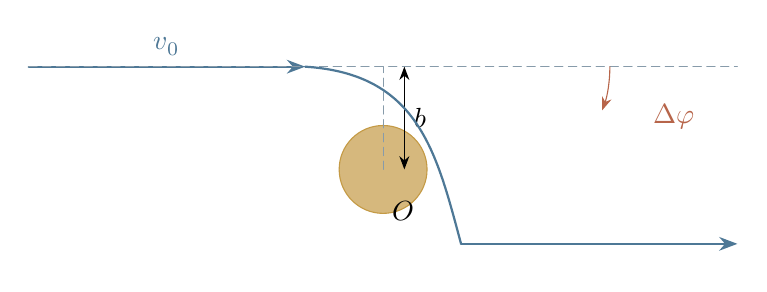
\begin{tikzpicture}[>=Stealth,scale=0.9]
  \fill[ThesisGold!70] (0,0) circle (0.62);
  \draw[ThesisGold] (0,0) circle (0.62);
  \node[below=8pt] at (0,0) {太阳中心 $O$};
  \draw[->,thick,ThesisBlue] (-5,1.45) -- (-1.1,1.45) node[midway,above] {$v_0$};
  \draw[->,thick,ThesisBlue] (1.1,-1.05) -- (5,-1.05) node[midway,below] {飞出方向};
  \draw[densely dashed,ThesisNavy!55] (-5,1.45) -- (5,1.45);
  \draw[densely dashed,ThesisNavy!55] (0,0) -- (0,1.45);
  \draw[<->] (0.3,0) -- (0.3,1.45) node[midway,right] {$b$};
  \draw[thick,ThesisBlue] (-1.1,1.45) .. controls (0.5,1.35) and (0.75,0.25) .. (1.1,-1.05);
  \draw[->,ThesisRust] (3.2,1.45) arc[start angle=0,end angle=-20,radius=1.8];
  \node[ThesisRust] at (4.1,0.75) {$\Delta\varphi$};
\end{tikzpicture}
\caption{太阳引力场中弱偏转问题的条件示意图（依据题意自绘）。}
\end{figure}

本问的核心任务不是直接记忆偏转角公式，而是把初始条件、轨道关系和出射方向的几何关系连成同一条推理链。弱偏转下，牛顿力学框架给出

\[
\Delta\varphi_{\mathrm{N}}
  \simeq \frac{2GM_\odot}{b v_0^2}.
\]

对掠日星光，在同一牛顿框架中代入 \(v_0=c\)、\(b=R_\odot\)，得到

\[
\Delta\varphi_{\mathrm{N,\,light}}
  \simeq \frac{2GM_\odot}{c^2R_\odot}.
\]

原题下一问再用弱场广义相对论的等效折射率模型重新计算，因此掠日星光的偏折为

\[
\Delta\varphi_{\mathrm{GR}}
  \simeq \frac{4GM_\odot}{c^2R_\odot}
  =2\,\Delta\varphi_{\mathrm{N,\,light}}.
\]

这里的系数差异来自模型的改变，而不是两道彼此无关的计算题。

\subsection{条件---关系链任务结构}\label{ux6761ux4ef6ux5173ux7cfbux94feux4efbux52a1ux7ed3ux6784}

该小问要求在两种给定情形下求飞出方向相对原飞入方向的偏转角。V3记录为模型建构L3、科学推理L3，科学论证和质疑创新均未出现。

该案例可用于设计``先列条件、再确定关系、最后说明结果适用情形''的任务。学生产出可以是条件表、偏转角关系式和对两种情形的分别说明；教师评价的对象应是条件是否进入推理链，而不是只核对最终公式。此处不据此推断学生一定会在条件识别上遇到困难。

从题设到解答的结构可分为三个可定位环节。第一，题目把入射物体的两种情形并列给出，并将``飞出方向相对原飞入方向的偏转角''固定为共同的待求量；第二，解答需要建立轨道对象、初始量、弱偏转近似和渐近方向之间的模型联系；第三，再将能量、角动量、轨道参数和几何关系组织为连续推演。模型建构L3对应多项对象与边界条件的整合，科学推理L3对应多条物理关系共同约束偏转角。题面没有另设需要辩护的主张，也没有要求改变假设或设计替代方案，因而不计科学论证和质疑创新。

据此，案例教学不宜把``写出偏转角公式''作为唯一完成标志。可观察的产出包括：区分题设中的共同目标与分情形条件，在关系链图中标出能量/角动量、轨道参数和偏转角之间的连接，并说明替换入射条件后需要改变哪一环。它们构成后续作品分析的评价入口。

\begin{longtable}[]{@{}
  >{\raggedright\arraybackslash}p{(\linewidth - 4\tabcolsep) * \real{0.3333}}
  >{\raggedright\arraybackslash}p{(\linewidth - 4\tabcolsep) * \real{0.3333}}
  >{\raggedright\arraybackslash}p{(\linewidth - 4\tabcolsep) * \real{0.3333}}@{}}
\caption{引力偏转案例的任务结构与学习产出}\tabularnewline
\toprule\noalign{}
\rowcolor{ThesisPale}
\begin{minipage}[b]{\linewidth}\raggedright
任务环节
\end{minipage} & \begin{minipage}[b]{\linewidth}\raggedright
题设或解答中的结构作用
\end{minipage} & \begin{minipage}[b]{\linewidth}\raggedright
可收集的书面产出
\end{minipage} \\
\midrule\noalign{}
\endfirsthead
\toprule\noalign{}
\rowcolor{ThesisPale}
\begin{minipage}[b]{\linewidth}\raggedright
任务环节
\end{minipage} & \begin{minipage}[b]{\linewidth}\raggedright
题设或解答中的结构作用
\end{minipage} & \begin{minipage}[b]{\linewidth}\raggedright
可收集的书面产出
\end{minipage} \\
\midrule\noalign{}
\endhead
\bottomrule\noalign{}
\endlastfoot
条件辨识 & 区分两种入射情形及其速度、瞄准距离等条件 &
条件表，标明共同条件和分情形条件 \\
关系组织 & 将轨道参数、初始条件与偏转角关系串联 &
带有条件/原理标注的关系链图 \\
结果说明 & 用同一待求量比较两种情形 & 分情形结论与适用条件说明 \\
边界核对 & 改变一个关键条件时检查关系链 & ``哪一步需重检''的文字说明 \\
\end{longtable}

\section{案例二：状态分类与平均能量关系}\label{ux6848ux4f8bux4e8cux72b6ux6001ux5206ux7c7bux4e0eux5e73ux5747ux80fdux91cfux5173ux7cfb}

\subsection{题目导读与题干整理}\label{ux9898ux76eeux5bfcux8bfbux4e0eux9898ux5e72ux6574ux7406-1}

本题研究一个含有 \(N\) 个无相互作用电子的一维圆环。穿过圆环的磁通量为
\(\Phi\)，系统接近绝对零度，总能量取最小值。题目限定
\(-\dfrac{h}{2e}\leq\Phi\leq\dfrac{h}{2e}\)，要求给出单粒子平均能量随磁通量的变化关系，并比较
\(N\) 为奇数和偶数时，\(\Phi=0\) 与 \(|\Phi|=\dfrac{h}{2e}\)
两处的平均能量。

\begin{figure}[H]
\centering
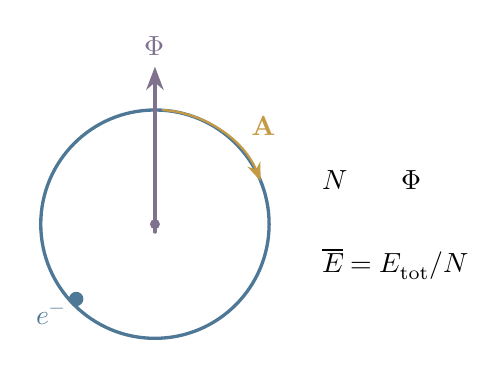
\begin{tikzpicture}[>=Stealth,scale=1.0]
  \draw[very thick,ThesisBlue] (0,0) circle (1.45);
  \draw[->,very thick,ThesisLavender] (0,-0.1) -- (0,2.0) node[above] {$\Phi$};
  \fill[ThesisLavender] (0,0) circle (1.8pt);
  \draw[->,thick,ThesisGold] (0.1,1.45) arc[start angle=86,end angle=22,radius=1.45];
  \node[ThesisGold,above right] at (1.1,1.0) {$\mathbf A$};
  \fill[ThesisBlue] (-1.0,-0.95) circle (2.6pt) node[below left] {$e^-$};
  \node[align=left,anchor=west] at (2.0,0.65) {分类条件：\\$N$ 的奇偶性与 $\Phi$ 的取值};
  \node[align=left,anchor=west] at (2.0,-0.45) {共同比较对象：\\$\overline E=E_{\mathrm{tot}}/N$};
\end{tikzpicture}
\caption{磁通穿过一维圆环的状态分类情境（依据题意自绘）。}
\end{figure}

题面要求围绕同一个平均能量对象进行分支讨论：

\[
-\frac{h}{2e}\leq \Phi\leq\frac{h}{2e},
\qquad
\overline{E}(\Phi)=\frac{E_{\mathrm{tot}}(\Phi)}{N}.
\]

令 \(N=2M+1\)（奇数）或 \(N=2M\)（偶数），\(M\)
为非负整数。参考解答将平均能量整理为下列分支形式，其中
\(\hbar=h/(2\pi)\)：

\[
\overline{E}_{\mathrm{odd}}(\Phi)
=\frac{e^2\Phi^2}{8\pi^2mR^2}
+\frac{\hbar^2}{2mR^2}\,\frac{M(M+1)}{3},
\qquad N=2M+1,
\]
\[
\overline{E}_{\mathrm{even}}(\Phi)
=\frac{\hbar^2}{2mR^2}
 \left(\left|\frac{e\Phi}{h}\right|-\frac12\right)^2
+\frac{\hbar^2}{2mR^2}
 \left(\frac{M^2}{3}-\frac1{12}\right),
\qquad N=2M.
\]

因此，磁通量区间和电子数奇偶性不是附带条件，而是决定能量表达式应如何分支的分类依据。

\subsection{状态分类任务结构}\label{ux72b6ux6001ux5206ux7c7bux4efbux52a1ux7ed3ux6784}

该小问要求给出系统单粒子平均能量随磁通变化的关系，并比较不同状态下的平均能量。V3记录为模型建构L3、科学推理L3、科学论证L2，质疑创新未出现。

该案例可用于设计``状态分类---能量表达---比较结论''的三段任务。可要求学生先明确分类依据，再分别写出可用表达式，最后以文字说明比较关系。评价记录应区分``完成代入''与``说明分类为何改变能量关系''。

该小问的结构重点不是单独计算某一数值，而是先确定何种分类会改变可用状态与表达式。题设要求给出平均能量随磁通变化的关系，参考解答则以磁通范围、前一问关系和粒子数奇偶为入口组织分支。模型建构L3对应系统条件、分类规则和平均能量表达的整体组织；科学推理L3对应从能级占据、粒子数奇偶和磁通区间到分段表达式的多步关系链；科学论证L2则体现在以共同物理量为对象，对不同状态和边界点的能量关系给出比较依据。

在教学设计中，可将``分类依据是否来自题设''\,``各分支是否比较同一物理量''\,``表达式是否与相应条件匹配''分别记录。这样的拆分可以避免把正确的最终比较结果误判为完整的模型组织过程，也能让教师在真实实施后定位作品中缺失的是条件提取、分支建立还是比较说明。这里并不预设学生会在哪一环出错，更不把当前编码等级投射为个体学习等级。

\begin{longtable}[]{@{}
  >{\raggedright\arraybackslash}p{(\linewidth - 4\tabcolsep) * \real{0.3333}}
  >{\raggedright\arraybackslash}p{(\linewidth - 4\tabcolsep) * \real{0.3333}}
  >{\raggedright\arraybackslash}p{(\linewidth - 4\tabcolsep) * \real{0.3333}}@{}}
\caption{量子环案例的任务结构与学习产出}\tabularnewline
\toprule\noalign{}
\rowcolor{ThesisPale}
\begin{minipage}[b]{\linewidth}\raggedright
任务环节
\end{minipage} & \begin{minipage}[b]{\linewidth}\raggedright
题设或解答中的结构作用
\end{minipage} & \begin{minipage}[b]{\linewidth}\raggedright
可收集的书面产出
\end{minipage} \\
\midrule\noalign{}
\endfirsthead
\toprule\noalign{}
\rowcolor{ThesisPale}
\begin{minipage}[b]{\linewidth}\raggedright
任务环节
\end{minipage} & \begin{minipage}[b]{\linewidth}\raggedright
题设或解答中的结构作用
\end{minipage} & \begin{minipage}[b]{\linewidth}\raggedright
可收集的书面产出
\end{minipage} \\
\midrule\noalign{}
\endhead
\bottomrule\noalign{}
\endlastfoot
分类依据 & 磁通范围、粒子数及已有关系决定分支 &
分类依据卡，逐项回指题设 \\
分支建模 & 不同条件对应不同状态条件与表达式 &
条件---表达式---推导三列表 \\
比较说明 & 以单粒子平均能量为共同对象比较分支 & 比较表与文字解释 \\
反向检查 & 改变区间或粒子数时重审分支 & 需要改写的列及理由 \\
\end{longtable}

\section{案例三：近似条件下的动力学建模}\label{ux6848ux4f8bux4e09ux8fd1ux4f3cux6761ux4ef6ux4e0bux7684ux52a8ux529bux5b66ux5efaux6a21}

\subsection{题目导读与题干整理}\label{ux9898ux76eeux5bfcux8bfbux4e0eux9898ux5e72ux6574ux7406-2}

本题用沿 \(z\) 轴传播的线偏振单色平面电磁波近似强激光。电子在 \(t=0\)
从原点沿 \(x\)--\(z\)
平面注入，入射角受给定范围限制；本问忽略辐射阻尼，要求求出电子可达到的最大能量以及对应的入射角。这里的阅读重点是：电场、磁场方向和几何限制共同决定了可以保留哪些变量与关系。

\begin{figure}[H]
\centering
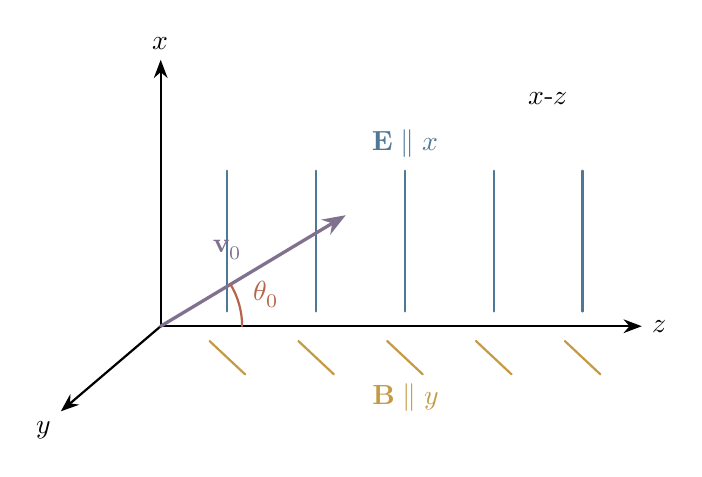
\begin{tikzpicture}[>=Stealth,scale=0.94]
  \draw[->,thick] (0,0) -- (6.5,0) node[right] {$z$};
  \draw[->,thick] (0,0) -- (0,3.6) node[above] {$x$};
  \draw[->,thick] (0,0) -- (-1.35,-1.15) node[below left] {$y$};
  \foreach \z in {0.9,2.1,3.3,4.5,5.7} {
    \draw[ThesisBlue,thick] (\z,0.2) -- (\z,2.1);
    \draw[ThesisGold,thick] (\z-0.24,-0.2) -- (\z+0.24,-0.65);
  }
  \node[ThesisBlue,above] at (3.3,2.15) {$\mathbf E\parallel x$};
  \node[ThesisGold,below] at (3.3,-0.65) {$\mathbf B\parallel y$};
  \draw[->,very thick,ThesisLavender] (0,0) -- (2.5,1.5) node[midway,above left] {$\mathbf v_0$};
  \draw[ThesisRust,thick] (1.1,0) arc[start angle=0,end angle=31,radius=1.1];
  \node[ThesisRust] at (1.42,0.43) {$\theta_0$};
  \node[align=left,anchor=south west] at (4.0,2.42) {电子初态：原点、$x$-$z$ 平面注入\\本问近似：忽略辐射阻尼};
\end{tikzpicture}
\caption{平面电磁波中电子注入的几何与场方向示意图（依据题意自绘）。}
\end{figure}

原题先给出电磁场表述，再对电子初始条件施加约束：

\[
\mathbf{E}(z,t)=E_0\cos\!\left(kz-\omega t\right)\mathbf{e}_x,
\qquad
\mathbf{B}(z,t)=\frac{E_0}{c}
\cos\!\left(kz-\omega t\right)\mathbf{e}_y.
\]
\[
\frac{\mathrm d\mathbf p}{\mathrm dt}
=-e\left(\mathbf E+\mathbf v\times\mathbf B\right),
\qquad
\varepsilon^2=p^2c^2+m_e^2c^4,
\qquad e>0.
\]

其中电子电荷为 \(-e\)。由 \(\mathbf e_x\times\mathbf e_y=\mathbf e_z\)
可见，电磁波能流沿 \(+z\) 方向；``沿 \(x\)--\(z\)
平面注入''和``忽略辐射阻尼''共同限定了后续最大能量问题的模型边界。

\subsection{近似条件建模任务结构}\label{ux8fd1ux4f3cux6761ux4ef6ux5efaux6a21ux4efbux52a1ux7ed3ux6784}

该小问在限定电子沿\texttt{x-z}平面注入、入射角范围及忽略辐射阻尼的条件下，要求求最大能量和相应入射角。V3记录为模型建构L3、科学推理L3，科学论证和质疑创新均未出现。

该案例适合用于呈现近似条件在任务中的功能：先让学生标出被限定的运动平面、角度范围和忽略项，再要求其说明这些条件分别减少了哪些未知量或约束了哪些关系。评价不应只依据最大能量的数值，还应保留学生对条件作用的书面说明。这里的``适合''是由题设结构推出的教学设计建议，不是课堂有效性的实证结论。

该题的解答显示，运动平面条件首先使一个动量分量为零，随后能量---动量关系、初始条件和入射角参数化被放到同一优化过程之中。题设中的``忽略辐射阻尼''并非装饰性背景，而是决定本小问采用何种简化动力学模型的限定；入射角范围则限定了后续极值条件的讨论范围。因此，模型建构L3和科学推理L3分别对应``如何在近似下组织变量与约束''和``如何将动力学关系、参数化与极值条件连成求解路径''。题目要求在给定近似下求解，并未要求评价该近似的局限、比较替代模型或提出新方案，所以不计科学论证和质疑创新。

将此类任务转化为教学材料时，可把``条件的功能''而不是``条件的名称''作为评价焦点。比如，学习者需用文字说明平面限制去除了什么变量、忽略项改变了什么模型边界、入射角如何进入最大能量的条件。只有在真实课堂中收集了这些说明、题面版本和修订痕迹后，才能讨论学生是否能够使用近似条件；本案例仅提出可收集的证据格式。

\begin{longtable}[]{@{}
  >{\raggedright\arraybackslash}p{(\linewidth - 4\tabcolsep) * \real{0.3333}}
  >{\raggedright\arraybackslash}p{(\linewidth - 4\tabcolsep) * \real{0.3333}}
  >{\raggedright\arraybackslash}p{(\linewidth - 4\tabcolsep) * \real{0.3333}}@{}}
\caption{强激光场电子加速案例的任务结构与学习产出}\tabularnewline
\toprule\noalign{}
\rowcolor{ThesisPale}
\begin{minipage}[b]{\linewidth}\raggedright
任务环节
\end{minipage} & \begin{minipage}[b]{\linewidth}\raggedright
题设或解答中的结构作用
\end{minipage} & \begin{minipage}[b]{\linewidth}\raggedright
可收集的书面产出
\end{minipage} \\
\midrule\noalign{}
\endfirsthead
\toprule\noalign{}
\rowcolor{ThesisPale}
\begin{minipage}[b]{\linewidth}\raggedright
任务环节
\end{minipage} & \begin{minipage}[b]{\linewidth}\raggedright
题设或解答中的结构作用
\end{minipage} & \begin{minipage}[b]{\linewidth}\raggedright
可收集的书面产出
\end{minipage} \\
\midrule\noalign{}
\endhead
\bottomrule\noalign{}
\endlastfoot
条件标注 & 运动平面、入射角范围和忽略项构成约束 & 条件---变量对照表 \\
模型简化 & 条件决定保留或排除的动力学因素 & 简化说明与适用边界句 \\
关系推演 & 能量---动量关系、参数化和极值条件共同出现 &
带有依据的求解路线图 \\
结果核对 & 最大值及相应角度需回到限制条件 & 结果---条件一致性说明 \\
\end{longtable}

\section{案例四：旋转谐振腔的频率分裂}\label{ux6848ux4f8bux56dbux65cbux8f6cux8c10ux632fux8154ux7684ux9891ux7387ux5206ux88c2}

\subsection{题目导读与题干整理}\label{ux9898ux76eeux5bfcux8bfbux4e0eux9898ux5e72ux6574ux7406-3}

第37届复赛第6题第（3）问讨论谐振式光学陀螺仪。半径为 \(R\)
的环形腔以角速度 \(\Omega\) 沿逆时针方向旋转，腔中介质折射率为
\(n_1\)，并满足
\(R\Omega\ll c\)。腔内同时存在顺时针与逆时针传播的共振模式；题目特别规定比较的是\textbf{同一级次}
\(m\) 的两类模式，要求导出角速度与共振频率差 \(\Delta f\) 的关系。

\begin{figure}[H]
\centering
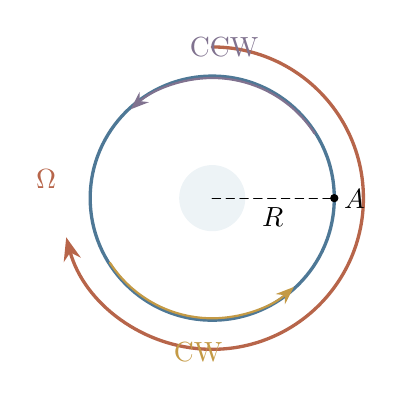
\begin{tikzpicture}[>=Stealth,scale=1.0]
  \draw[very thick,ThesisBlue] (0,0) circle (1.55);
  \fill[ThesisPale] (0,0) circle (0.42);
  \node at (0,0) {腔体};
  \draw[->,very thick,ThesisRust] (0,1.92) arc[start angle=90,end angle=-165,radius=1.92];
  \node[ThesisRust] at (-2.1,0.25) {$\Omega$};
  \draw[->,thick,ThesisLavender] (1.30,0.82) arc[start angle=33,end angle=132,radius=1.55];
  \node[ThesisLavender] at (0.15,1.92) {CCW};
  \draw[->,thick,ThesisGold] (-1.30,-0.82) arc[start angle=213,end angle=312,radius=1.55];
  \node[ThesisGold] at (-0.18,-1.95) {CW};
  \draw[densely dashed] (0,0) -- (1.55,0) node[midway,below] {$R$};
  \fill (1.55,0) circle (1.5pt) node[right] {$A$};
\end{tikzpicture}
\caption{旋转光学环形腔中两类共振模式的示意图（依据题意自绘）。}
\end{figure}

静止时，环形腔的周期边界条件给出

\[
2\pi R=m\lambda_{m0}.
\]

旋转后，同一 \(m\)
值的两类模式因传播方向不同而有不同的共振频率。参考解答先保留旋转修正，再利用
\(R\Omega\ll c\) 作近似，得到

\[
\Delta f
=\frac{m\Omega}{\pi}
 \frac{c^2-(\Omega R)^2}{c^2-(n_1\Omega R)^2}
\simeq\frac{m\Omega}{\pi},
\qquad
\Omega=\frac{\pi}{m}\Delta f
=\frac{\lambda_{m0}}{2R}\Delta f .
\]

上式中
\(\Delta f=f_{\mathrm{CW}}-f_{\mathrm{CCW}}\)；若改变频率差的正方向约定，式子的符号也应相应改变。题目要点不在于背诵最终比例式，而在于说明``同一级次''\,``旋转方向''和``小量近似''分别在比较中起什么作用。

\subsection{同模式比较任务结构}\label{ux540cux6a21ux5f0fux6bd4ux8f83ux4efbux52a1ux7ed3ux6784}

该小问的V3记录为模型建构L3、科学推理L3，科学论证和质疑创新均未出现。解题者需要把环形腔的周期边界、同一模式级次、顺逆时针传播、腔体旋转和小量近似组织为同一个比较模型，并由精确频率关系推到一阶近似式。两个L3分别对应多项模型条件的整合和多条关系的连续推演；题目没有设置需要以证据辩护的独立主张，也没有要求改变方案。

教学中可先让学生填写``保持不变---发生改变---比较结果''三栏：保持不变的是模式级次
\(m\) 和腔体半径
\(R\)，发生改变的是两束光相对旋转腔的传播方向，比较结果是两类模式的频率差。随后再追问：若不声明
\(R\Omega\ll c\)，哪一步不能直接把精确表达式化为线性比例关系。这样可把近似条件从公式末尾的符号变成可解释的物理限制。

\begin{longtable}[]{@{}
  >{\raggedright\arraybackslash}p{(\linewidth - 4\tabcolsep) * \real{0.3333}}
  >{\raggedright\arraybackslash}p{(\linewidth - 4\tabcolsep) * \real{0.3333}}
  >{\raggedright\arraybackslash}p{(\linewidth - 4\tabcolsep) * \real{0.3333}}@{}}
\caption{旋转谐振腔案例的任务结构与学习产出}\tabularnewline
\toprule\noalign{}
\rowcolor{ThesisPale}
\begin{minipage}[b]{\linewidth}\raggedright
任务环节
\end{minipage} & \begin{minipage}[b]{\linewidth}\raggedright
题设或解答中的结构作用
\end{minipage} & \begin{minipage}[b]{\linewidth}\raggedright
可收集的书面产出
\end{minipage} \\
\midrule\noalign{}
\endfirsthead
\toprule\noalign{}
\rowcolor{ThesisPale}
\begin{minipage}[b]{\linewidth}\raggedright
任务环节
\end{minipage} & \begin{minipage}[b]{\linewidth}\raggedright
题设或解答中的结构作用
\end{minipage} & \begin{minipage}[b]{\linewidth}\raggedright
可收集的书面产出
\end{minipage} \\
\midrule\noalign{}
\endhead
\bottomrule\noalign{}
\endlastfoot
比较对象固定 & 同一级次 \(m\) 的CW、CCW模式才可直接比较 &
``不变量---变量''对照表 \\
周期条件调用 & 环形边界把模式级次与波长联系起来 & 标注
\(2\pi R=m\lambda_{m0}\) 含义的关系图 \\
近似判断 & \(R\Omega\ll c\) 决定是否可保留一阶关系 &
精确式到近似式的条件说明 \\
结论解释 & 频率差的正负依赖方向约定 & 写明 \(\Delta f\) 定义的结论句 \\
\end{longtable}

\section{案例五：可动楔块上的纯滚动条件}\label{ux6848ux4f8bux4e94ux53efux52a8ux6954ux5757ux4e0aux7684ux7eafux6edaux52a8ux6761ux4ef6}

\subsection{题目导读与题干整理}\label{ux9898ux76eeux5bfcux8bfbux4e0eux9898ux5e72ux6574ux7406-4}

第40届复赛第3题第（1）问给出质量为 \(M\) 的楔块和质量为 \(m\)、半径为
\(r\) 的匀质圆球。楔块可在光滑水平面上运动，圆球在倾角为 \(\theta\)
的斜面上向下滚动。题目要求在圆球相对楔块纯滚动的条件下，求楔块和圆球的加速度，并进一步确定维持纯滚动所需的最小静摩擦因数。

\begin{figure}[H]
\centering
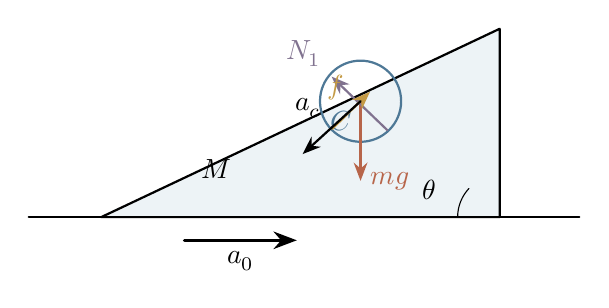
\begin{tikzpicture}[>=Stealth,scale=0.92]
  \draw[thick] (-3.8,-1.45) -- (3.8,-1.45);
  \fill[ThesisPale] (-2.8,-1.45) -- (2.7,-1.45) -- (2.7,1.15) -- cycle;
  \draw[thick] (-2.8,-1.45) -- (2.7,-1.45) -- (2.7,1.15) -- cycle;
  \draw[thick,ThesisBlue] (0.78,0.15) circle (0.56);
  \fill[ThesisBlue] (0.78,0.15) circle (1.6pt) node[below left] {$C$};
  \draw[->,thick,ThesisRust] (0.78,0.15) -- (0.78,-0.95) node[right] {$mg$};
  \draw[->,thick,ThesisLavender] (1.15,-0.25) -- (0.38,0.49) node[above left] {$N_1$};
  \draw[->,thick,ThesisGold] (0.39,-0.23) -- (0.91,0.28) node[midway,above left] {$f$};
  \draw[->,very thick] (-1.65,-1.77) -- (-0.1,-1.77) node[midway,below] {$a_0$};
  \draw[->,thick] (0.78,0.15) -- (-0.02,-0.58) node[midway,above left] {$a_c$};
  \draw (2.12,-1.45) arc[start angle=180,end angle=137,radius=0.58];
  \node at (1.73,-1.08) {$\theta$};
  \node at (-1.4,-0.78) {楔块 $M$};
\end{tikzpicture}
\caption{可动楔块上圆球纯滚动的受力与加速度方向示意图（依据题意自绘）。}
\end{figure}

本题同时出现平动、转动和楔块水平运动三类关系。以沿斜面向下为正，参考解答使用匀质球转动惯量和无滑动约束

\[
I_C=\frac{2}{5}mr^2,
\qquad a_c=r\ddot\varphi,
\qquad
m(a_c\cos\theta-a_0)=Ma_0.
\]

联立斜面方向受力、转动方程和整体的水平关系，可得

\[
a_0=\frac{5mg\sin\theta\cos\theta}
{7(M+m)-5m\cos^2\theta},
\qquad
a_c=\frac{5(M+m)g\sin\theta}
{7(M+m)-5m\cos^2\theta},
\]
\[
\mu_0=\frac{2(M+m)}{7M+2m}\tan\theta.
\]

最后一个结果是``最小静摩擦因数''，不是任意滑动情形下的动摩擦因数。它来自纯滚动约束仍能满足时摩擦力与法向力之比的边界值。

\subsection{多对象约束联立任务结构}\label{ux591aux5bf9ux8c61ux7ea6ux675fux8054ux7acbux4efbux52a1ux7ed3ux6784}

第（1）问在V3中按五个独立待求量拆为五个分析单元：求楔块对地加速度时为模型建构L3、科学推理L3；求圆球质心相对楔块加速度时模型建构未出现、科学推理L1；求地面对楔块支持力时为模型建构L2、科学推理L2；求楔块对圆球支持力时为模型建构L2、科学推理L2；求最小摩擦因数时为模型建构L1、科学推理L2。五个单元的科学论证和质疑创新均未出现。

这种拆分保留了同一大题内部的任务变化。第一个待求量需要协调圆球、楔块和整体的多对象模型，后续待求量则在已经建立的模型基础上调用局部关系或增加一项受力、边界判断，不能把第一个单元的L3标签复制给整个第（1）问。该案例的代表性正在于：同一连续解答中，不同输出对模型组织和关系推演的要求并不相同。

教学中可将题目拆为``先画谁''\,``再写哪一类方程''\,``最后检查哪一个边界''三个问题。先要求学生分别标出圆球、楔块和整体的研究对象；再要求说明每条方程对应平动、转动还是整体水平方向；最后用
\(\mu=f/N_1\)
核对所得摩擦系数是否是使纯滚动恰好成立的临界值。这样既不把复杂题化为套公式，也避免学生把固定斜面结论直接搬到可动楔块上。

\begin{longtable}[]{@{}
  >{\raggedright\arraybackslash}p{(\linewidth - 4\tabcolsep) * \real{0.3333}}
  >{\raggedright\arraybackslash}p{(\linewidth - 4\tabcolsep) * \real{0.3333}}
  >{\raggedright\arraybackslash}p{(\linewidth - 4\tabcolsep) * \real{0.3333}}@{}}
\caption{可动楔块纯滚动案例的任务结构与学习产出}\tabularnewline
\toprule\noalign{}
\rowcolor{ThesisPale}
\begin{minipage}[b]{\linewidth}\raggedright
任务环节
\end{minipage} & \begin{minipage}[b]{\linewidth}\raggedright
题设或解答中的结构作用
\end{minipage} & \begin{minipage}[b]{\linewidth}\raggedright
可收集的书面产出
\end{minipage} \\
\midrule\noalign{}
\endfirsthead
\toprule\noalign{}
\rowcolor{ThesisPale}
\begin{minipage}[b]{\linewidth}\raggedright
任务环节
\end{minipage} & \begin{minipage}[b]{\linewidth}\raggedright
题设或解答中的结构作用
\end{minipage} & \begin{minipage}[b]{\linewidth}\raggedright
可收集的书面产出
\end{minipage} \\
\midrule\noalign{}
\endhead
\bottomrule\noalign{}
\endlastfoot
研究对象划分 & 圆球、楔块与整体对应不同方程入口 &
三个对象的受力或运动图 \\
约束连接 & 纯滚动把线加速度与角加速度联系起来 & 标出
\(a_c=r\ddot\varphi\) 的方程卡 \\
方程联立 & 平动、转动与整体水平关系必须同时满足 &
方程旁标明``作用对象---方向---物理依据'' \\
边界检验 & \(\mu_0\) 对应纯滚动即将失效的临界条件 & 对 \(\mu_0=f/N_1\)
的文字解释 \\
\end{longtable}

\section{案例六：分层大气中的声波折射}\label{ux6848ux4f8bux516dux5206ux5c42ux5927ux6c14ux4e2dux7684ux58f0ux6ce2ux6298ux5c04}

\subsection{题目导读与题干整理}\label{ux9898ux76eeux5bfcux8bfbux4e0eux9898ux5e72ux6574ux7406-5}

第40届复赛第7题第（3）问把大气简化为平面分层介质：对流层和逆温层温度均为
\(-10\,^{\circ}\mathrm C\)，同温层温度为
\(-55\,^{\circ}\mathrm C\)。声源位于同温层内，声波射向同温层与相邻大气层的界面。题目要求判断不同入射角下何时有折射，何时发生全反射，并作定性传播图。

\begin{figure}[H]
\centering
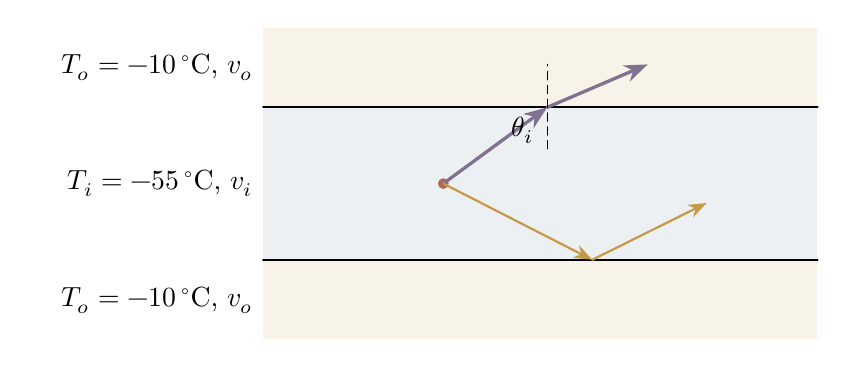
\begin{tikzpicture}[>=Stealth,scale=0.88]
  \fill[ThesisGold!12] (-4,1.1) rectangle (4,2.25);
  \fill[ThesisBlue!11] (-4,-1.1) rectangle (4,1.1);
  \fill[ThesisGold!12] (-4,-2.25) rectangle (4,-1.1);
  \draw[thick] (-4,1.1) -- (4,1.1);
  \draw[thick] (-4,-1.1) -- (4,-1.1);
  \node[left] at (-4,1.68) {外层：$T_o=-10\,^{\circ}\mathrm C$, $v_o$};
  \node[left] at (-4,0) {同温层：$T_i=-55\,^{\circ}\mathrm C$, $v_i$};
  \node[left] at (-4,-1.68) {外层：$T_o=-10\,^{\circ}\mathrm C$, $v_o$};
  \fill[ThesisRust] (-1.4,0) circle (2.2pt) node[below] {声源};
  \draw[->,very thick,ThesisLavender] (-1.4,0) -- (0.1,1.1);
  \draw[->,very thick,ThesisLavender] (0.1,1.1) -- (1.55,1.72);
  \draw[densely dashed] (0.1,0.5) -- (0.1,1.72);
  \draw[->,thick,ThesisGold] (-1.4,0) -- (0.75,-1.1);
  \draw[->,thick,ThesisGold] (0.75,-1.1) -- (2.4,-0.28);
  \node[ThesisLavender] at (1.5,1.25) {折射};
  \node[ThesisGold] at (2.25,-0.72) {全反射示意};
  \node at (-0.25,0.77) {$\theta_i$};
\end{tikzpicture}
\caption{同温层内声波射向界面时的折射与全反射示意图（依据题意自绘）。}
\end{figure}

声速由绝热声速关系决定：

\[
v_s^2=\gamma\frac{p}{\rho}=\frac{\gamma RT}{\mu}.
\]

因此，题设给出的温度意味着
\(v_o/v_i=\sqrt{263.15/218.15}\simeq1.098\)。以界面法线为基准测量入射角
\(\theta_i\)，折射关系和临界角为

\[
\sin\theta_o=\frac{v_o}{v_i}\sin\theta_i,
\qquad
\theta_{im}=\arcsin\!\left(\frac{v_i}{v_o}\right)
\simeq65.6^{\circ}.
\]

当 \(\theta_i<\theta_{im}\) 时可同时出现折射与反射；当
\(\theta_i>\theta_{im}\) 时不存在满足折射关系的实数
\(\theta_o\)，声波在同温层内发生全反射。这里的``临界角''不是凭图形直觉给出的，而是由温度先决定声速比、声速比再限制折射角的存在性。

\subsection{分层介质的条件分支任务结构}\label{ux5206ux5c42ux4ecbux8d28ux7684ux6761ux4ef6ux5206ux652fux4efbux52a1ux7ed3ux6784}

该小问的V3记录为模型建构L3、科学推理L3、科学论证L2，质疑创新未出现。题面将连续变化的大气简化为若干等温层，解题者还需组织不同层的温度、声速、界面法线、入射方向和折射条件。由温度关系得到声速比，再由折射定律确定临界角并区分折射与全反射，构成多条件、多关系的推演链；对两种传播情形给出条件依据构成L2科学论证。题目没有要求修改分层模型或另行设计传播方案，因而不计质疑创新。

适合的课堂任务不是一开始就要求画出``漂亮的光线图''，而是先让学生填写两步判断：第一步，根据
\(v_s\propto\sqrt T\) 判断哪一层声速更大；第二步，依据
\(\sin\theta_o=(v_o/v_i)\sin\theta_i\)
判断何时右端会超过1。图形应当是前两步判断的表达结果，而不是独立的作图技巧。这样也能避免把温度高低、声速大小和全反射条件混为三件互不相干的事。

\begin{longtable}[]{@{}
  >{\raggedright\arraybackslash}p{(\linewidth - 4\tabcolsep) * \real{0.3333}}
  >{\raggedright\arraybackslash}p{(\linewidth - 4\tabcolsep) * \real{0.3333}}
  >{\raggedright\arraybackslash}p{(\linewidth - 4\tabcolsep) * \real{0.3333}}@{}}
\caption{分层大气声波折射案例的任务结构与学习产出}\tabularnewline
\toprule\noalign{}
\rowcolor{ThesisPale}
\begin{minipage}[b]{\linewidth}\raggedright
任务环节
\end{minipage} & \begin{minipage}[b]{\linewidth}\raggedright
题设或解答中的结构作用
\end{minipage} & \begin{minipage}[b]{\linewidth}\raggedright
可收集的书面产出
\end{minipage} \\
\midrule\noalign{}
\endfirsthead
\toprule\noalign{}
\rowcolor{ThesisPale}
\begin{minipage}[b]{\linewidth}\raggedright
任务环节
\end{minipage} & \begin{minipage}[b]{\linewidth}\raggedright
题设或解答中的结构作用
\end{minipage} & \begin{minipage}[b]{\linewidth}\raggedright
可收集的书面产出
\end{minipage} \\
\midrule\noalign{}
\endhead
\bottomrule\noalign{}
\endlastfoot
分层建模 & 将不同高度的连续大气简化为等温层与平面界面 &
标注温度和声速的分层图 \\
量值比较 & 温度决定两侧声速比 & 从 \(T\) 到 \(v_s\) 的一行推理 \\
条件分支 & 折射角是否存在决定折射或全反射 & \(\theta_i\) 与
\(\theta_{im}\) 的判断表 \\
图示解释 & 射线图要对应已写出的条件判断 &
图中标注法线、入射角和传播情形 \\
\end{longtable}

\section{跨案例任务结构比较}\label{ux8de8ux6848ux4f8bux4efbux52a1ux7ed3ux6784ux6bd4ux8f83}

\subsection{六类物理情境中的共同结构}\label{ux516dux7c7bux7269ux7406ux60c5ux5883ux4e2dux7684ux5171ux540cux7ed3ux6784}

六个案例覆盖引力、量子、强激光、光学陀螺、刚体力学和大气声学六类情境，物理内容差异很大，却都包含``从题面条件进入关系组织''的共同结构。偏转角案例把共同目标与分情形条件放入推理路径；量子环案例按磁通范围与粒子数建立分支；电子加速案例要求把几何限制和忽略项变成模型边界；谐振腔案例要求固定比较对象并说明近似；可动楔块案例要求协调多个研究对象与运动约束；声波折射案例则把温度分层转化为声速比和临界角判断。

从模型建构角度看，六案的差别在于模型条件的呈现方式。量子环的分类规则、电子加速的近似边界、楔块问题的多对象约束以及大气问题的分层简化，都要求解题者先决定哪些条件应进入工作模型；偏转角和谐振腔的基本模型相对明确，但仍须正确使用入射条件、模式级次和方向约定。由此可形成由``在既定模型内调用条件''到``依据条件协调模型和约束''的训练梯度。

从科学推理角度看，六案的关系组织形式也不同：偏转角是连续推演链，量子环是条件分支，电子加速是约束下的参数化与极值，谐振腔是同类模式的比较，楔块问题是方程联立，声波折射是阈值判断。把这些结构先画成关系图、分类表、对象图或判断表，能使学生在进行计算之前看见推理的骨架。

从评价角度看，六类任务都应兼顾结果与过程。教师既可检查最终表达式或图示，也可检查条件是否进入相应关系、比较对象是否保持一致、约束方程是否对应正确对象、临界判断是否有量值依据。评价重点不只是区分``算对''与``算错''，而是定位条件提取、模型组织、关系推演和结论说明中的具体缺口。

\subsection{基于六则案例的递进式任务设计}\label{ux57faux4e8eux516dux5219ux6848ux4f8bux7684ux9012ux8fdbux5f0fux4efbux52a1ux8bbeux8ba1}

六则案例可以组成由关系调用到模型组织、再到条件修正的递进序列。第一层可从偏转角和声波折射案例开始：前者要求把变化的入射条件放入同一条关系链，后者要求把温度差转化为声速比和临界条件。学生先完成条件表或判断表，再进入代数推演和图示表达。

第二层可转入谐振腔和量子环案例。前者要求固定同一模式级次后比较两个方向的频率，后者要求根据磁通范围和粒子数选择分支表达式；二者都强调``比较对象不变、分类条件清楚''。教学中可先提供不完整的条件卡，再要求学生补成比较表或分支图。

第三层可使用可动楔块和近似条件下的电子加速案例。学生须分别组织多个受力/运动对象，或解释运动平面、入射角范围和忽略项对模型的限制。此时的任务不只是调用关系，更要求说明哪条约束、哪种近似使某组方程可以成立。

三层递进并不等同于唯一教学顺序。递进的核心是任务要求从识别条件进入单一关系，发展到依据条件建立比较或分支，再到协调多个约束并审查模型边界。不同物理模块可以围绕这条主线形成连续训练。

在每一层任务结束后，教师可采用``展示产出---同伴比较---修订说明''的简短反馈程序。展示产出不是只展示最终答案，而是展示条件表、关系图、分支表或近似说明；同伴比较关注是否遗漏条件、是否混淆比较对象、是否把近似条件误作计算步骤；修订说明则要求学生写出自己修改了哪一处、为什么修改。这样形成的记录能使竞赛训练中的思维过程留下可讨论的痕迹，也为后续针对性评讲提供依据。

\section{基于任务结构的教学设计启示}\label{ux57faux4e8eux4efbux52a1ux7ed3ux6784ux7684ux6559ux5b66ux8bbeux8ba1ux542fux793a}

\subsection{任务、支架、产出与反馈}\label{ux4efbux52a1ux652fux67b6ux4ea7ux51faux4e0eux53cdux9988}

六个案例共同形成``任务结构---学习任务---支架---可观察产出---反馈要点''的设计链条。任务结构说明题目的关键工作，学习任务规定学生需要完成什么，支架帮助学生进入复杂问题，可观察产出为检查提供依据，反馈要点则把学生作品重新带回条件、模型、关系与结论边界。

\begin{longtable}[]{@{}
  >{\raggedright\arraybackslash}p{(\linewidth - 6\tabcolsep) * \real{0.2500}}
  >{\raggedright\arraybackslash}p{(\linewidth - 6\tabcolsep) * \real{0.2500}}
  >{\raggedright\arraybackslash}p{(\linewidth - 6\tabcolsep) * \real{0.2500}}
  >{\raggedright\arraybackslash}p{(\linewidth - 6\tabcolsep) * \real{0.2500}}@{}}
\caption{六类任务结构的教学设计启示}\tabularnewline
\toprule\noalign{}
\rowcolor{ThesisPale}
\begin{minipage}[b]{\linewidth}\raggedright
任务结构
\end{minipage} & \begin{minipage}[b]{\linewidth}\raggedright
学习任务与可观察产出
\end{minipage} & \begin{minipage}[b]{\linewidth}\raggedright
可提供的支架
\end{minipage} & \begin{minipage}[b]{\linewidth}\raggedright
反馈要点
\end{minipage} \\
\midrule\noalign{}
\endfirsthead
\toprule\noalign{}
\rowcolor{ThesisPale}
\begin{minipage}[b]{\linewidth}\raggedright
任务结构
\end{minipage} & \begin{minipage}[b]{\linewidth}\raggedright
学习任务与可观察产出
\end{minipage} & \begin{minipage}[b]{\linewidth}\raggedright
可提供的支架
\end{minipage} & \begin{minipage}[b]{\linewidth}\raggedright
反馈要点
\end{minipage} \\
\midrule\noalign{}
\endhead
\bottomrule\noalign{}
\endlastfoot
条件---关系链 & 条件表、关系式和适用情形说明 & 将已知、假设和待求量分栏
& 条件是否进入相应推理步骤 \\
状态分类---比较 & 分类依据、分情形表达式和比较结论 &
用状态卡或分支流程图组织讨论 & 分类是否完整、比较是否回到同一物理量 \\
近似条件建模 & 忽略项清单、受限变量和目标量关系 &
在题面中标注近似条件并追问其作用 & 是否说明条件改变了模型的哪些部分 \\
同对象比较 & 不变量、方向约定与近似前后表达式 & 比较对象卡与近似条件提示
& 是否固定同一模式或同一物理量 \\
多对象约束 & 对象图、约束式与联立方程 & 受力图和``对象---方向---方程''表
& 方程是否与对应对象、方向和约束一致 \\
阈值判断 & 量值比较、临界条件与传播图 &
``比例关系---是否超过1---图示''流程卡 & 临界角或边界是否由关系式推出 \\
\end{longtable}

上述建议可用于后续教学方案、教师案例评审或学生作答分析的设计。本文的证据来自试题与参考解答，因而不将这些评价项目表述为已经观察到的学习结果或已经验证的教学效果。

\subsection{教学任务序列设计}\label{ux6559ux5b66ux4efbux52a1ux5e8fux5217ux8bbeux8ba1}

依据六个案例的任务结构，竞赛教学可将一道综合题组织为``条件识别---关系组织---结果解释---边界核对''四个连续环节。条件识别阶段要求学生从题面中区分已知量、待求量、限制条件和近似假设，并说明这些信息分别属于研究对象、模型边界还是求解目标。关系组织阶段要求学生将条件与所用规律连接起来，可采用条件表、关系图、对象图或分支流程图呈现。结果解释阶段不只写出计算结果，还要求说明结果对应的物理情形和比较对象。边界核对阶段则通过改变条件、考察极限或比较相邻情形，检查结论是否仍然适用。

这一序列并不意味着每一道题都必须增加相同数量的书面步骤，而是为教师识别任务重点提供框架。对于以条件---关系链为主的题目，可将条件表和关系图作为主要产出；对于状态分类题，可将分类依据和分支表达式作为主要产出；对于近似条件题，则应重点要求学生解释忽略项、变量约束和模型适用范围。由此，教学任务的难度不只由计算量决定，还可以通过减少或增加需要显性表达的关系、比较和说明来调节。

在反馈方式上，教师可先根据学生的书面产出判断问题发生在哪一环：若条件未被识别，应回到题面标注与变量说明；若条件已被识别但未进入推演，应要求补充``条件---规律---结论''的连接；若计算正确但解释不足，则可追问比较对象、近似条件或结论适用范围。这样的反馈针对可观察的任务产出，不预设学生具有某种固定能力标签，也便于在后续真实教学中形成过程性记录。

\subsection{评价证据与反馈记录}\label{ux8bc4ux4ef7ux8bc1ux636eux4e0eux53cdux9988ux8bb0ux5f55}

为使评价与任务目标一致，可将每类书面产出划分为``是否呈现''\,``是否与题设对应''\,``是否能够支撑后续推理''三个观察维度。以条件表为例，首先检查是否列出关键条件，其次检查条件是否被正确归入共同条件、分情形条件或近似条件，最后检查这些条件是否在关系式、分支判断或结果说明中真正发挥作用。以比较结论为例，既要检查是否得到数值或符号关系，也要检查比较对象是否一致、结论是否说明适用条件。

评价记录不应直接把学生的单次作答换算成``模型建构L3''或``科学推理L2''等研究编码等级。论文中的编码等级用于描述试题任务要求，课堂评价则服务于理解学生作品中的具体表现，两者虽可在任务结构上相互参照，却属于不同层面的判断。将二者分开，可以避免用试题分析替代学习评价，也能使未来的教学研究在收集真实作品后保持清晰的证据边界。

六个案例的共同方法是把``题目要求''拆成可见的任务产出，而不是把题目编码直接翻译成对学习者的心理判断。除条件---关系链、状态分类和近似建模外，谐振腔案例强调比较对象与方向约定，楔块案例强调对象划分与约束联立，声波案例强调临界条件的量化判断。后续若开展教师案例评审，可请审查者只评价任务材料是否清楚、产出是否可观察、评价项是否可操作，并把教师对学生表现或课堂效果的判断另行记录，避免不同证据类型混为同一结论。

\subsection{竞赛题评讲的组织与反馈}\label{ux7adeux8d5bux9898ux8bc4ux8bb2ux7684ux7ec4ux7ec7ux4e0eux53cdux9988}

在竞赛题评讲中，教师通常容易从完整解答出发，按照公式推导顺序讲解。这样的方式能够保证解答的严谨性，却可能使学生只记住``下一步写什么''，而没有理解``为什么此处可以使用这一关系''。基于本研究的案例结构，评讲可改为在展示完整推导之前安排短暂的任务准备：先请学生标出研究对象、关键条件和待求量，再让学生预测可能需要的物理规律或比较关系。准备阶段不需要给出正确答案，其功能是让学生带着对条件和模型的判断进入后续推导。

进入正式推导后，教师可把板书或投影划分为``条件''\,``模型''\,``关系''\,``结论''四个区域。每写出一条关键方程，都要说明它对应哪一个模型假设、使用了题面中的哪一个条件、对后续结论产生了什么限制。例如，在偏转角任务中，需要指出入射条件如何决定轨道参数；在状态分类任务中，需要指出磁通范围和粒子数为何导致表达式分支；在近似条件任务中，需要指出忽略项为何允许采用特定的动力学关系。这样，公式不再被呈现为孤立的符号，而成为题设条件与物理结论之间的中间环节。

评讲的收束环节可围绕``结果是否回到题设''进行。教师可要求学生用一句话回答：本题中最关键的限制条件是什么，若改变这一条件，哪一步推导需要重新检查；也可以要求学生比较两种情形时保持同一物理量和同一参考对象。此类追问能够把极限、近似、分类和比较重新带回物理含义，避免学生只在计算结束后机械核对数值。对于开放程度较高的题目，还可以让学生提出一个可改变的假设，并说明改变后最先需要修订的是模型、关系式还是结论解释。

反馈应当围绕可见的作品而非笼统评价展开。若学生遗漏条件，教师可提示其回到条件表补充分类；若学生选对规律却未建立完整关系链，可要求其在箭头图中补出中间量；若学生计算正确但结论说明不充分，可要求其补写适用范围或比较依据。这样的反馈把``会不会做''分解为若干可修正的环节，既保留竞赛训练的高要求，也给学生提供了明确的改进方向。

从长期训练看，条件表、关系图、分支表和边界说明不必在每一道题中都以完整形式出现。教师可以在新题型或关键转折处使用完整支架，随着学生对任务结构的熟悉逐步减少提示，最终要求学生在草稿或口头说明中自主呈现这些关系。支架撤除的依据应是学生能否主动识别条件功能、组织推演链并说明结论边界，而不是单纯完成了多少道题。由此，竞赛题评讲能够兼顾效率与思维过程，使训练从答案模仿逐步走向对物理任务结构的自主把握。

教学设计的关键不是把竞赛题降低为若干零散技巧，而是在保持题目物理完整性的同时，为学生提供进入复杂任务的路径。条件识别帮助学生看见问题的约束，模型组织帮助学生确定可用的物理表达，关系推演帮助学生连接规律与目标，边界说明帮助学生理解结论的意义。四个环节相互衔接，既能够服务于单题评讲，也能够作为跨专题训练的共同结构。

这种共同结构还可以帮助教师安排练习的前后衔接。前一题训练的条件表和关系图，可以成为后一题建立分类分支或讨论近似边界的起点；后一题中出现的新限制条件，又可以反过来检验学生是否真正理解前一题所用模型的适用范围。于是，不同知识模块的竞赛题不再只是按章节并列，而能够围绕``识别条件---组织模型---推演关系---解释结论''的主线形成连续训练。这样的组织既尊重物理内容的差异，也使学生有机会在不同情境中重复使用和修正同一种思维工具。

在一组连续训练中，支架应当逐步撤除。初始阶段可以给出完整的条件表栏目、关系图框架和分类表头，使学生把注意力集中在信息的物理功能上；中间阶段只保留``共同条件''\,``分支依据''\,``适用范围''等提示词；后续阶段则要求学生根据题目性质自行选择合适的表示方式。撤除支架的依据不应是训练题数量，而应是学生能否主动说明条件的作用、关系的连接理由和结论的边界。该原则是教学设计建议，是否适合特定班级仍需由真实课堂材料检验。

教师还可将不同任务结构的评价结果用于调整下一轮选题。若多数学生在条件表中遗漏限制条件，下一轮宜选择模型明确但条件功能突出的题目；若学生能够列出条件却无法连接规律，可增加关系链短而变量转换清楚的任务；若学生计算正确但难以解释结论，可选择含有比较、极限或近似条件的题目，并把一句物理说明列为必答项。这样形成的调整依据是学生可见作品，而不是对学生能力作抽象判断。本文尚未收集这类作品，上述流程只说明未来实施时可以如何保存和使用证据。

上述六类任务均可形成可执行的教学设计。其中，条件---关系链任务要求学生从入射条件进入轨道关系；状态分类---比较任务要求先确定状态分支再比较同一物理量；近似条件建模任务要求说明近似如何限制变量与极值关系；其余三类则分别突出同对象比较、多对象约束和临界阈值判断。每类设计均可列出任务序列、支架撤除方式、可提交产出和评价记录，为备课、案例评审或课堂研究提供明确入口。

以条件---关系链任务为例，一次训练可分为四步。第一步，教师给出题目后只要求学生标注研究对象、共同条件、变化条件和待求量，暂不进入计算；第二步，学生以箭头图连接条件与可能使用的规律，并用一句话说明每个箭头的含义；第三步，学生完成正式推导，同时在关键公式旁标明它使用了哪一个条件；第四步，学生以极限情形、特殊值或两种情形的比较回看结论。四步的重点不在于增加书写形式，而在于使学生意识到推导不是公式的自然排列，而是由条件不断限制和推进的关系组织。

状态分类---比较任务的实施重点在于防止``先算后分''。教师可先隐去最终表达式，只提供描述系统状态的条件，让学生讨论哪些条件会改变可用的表达式，哪些条件只会改变参数取值；随后要求学生用表格列出每个分支的判据、表达式和比较对象；最后再完成代数计算。若学生得到不同分支下的结果，反馈不应只问哪个数值正确，还应追问分支边界是否覆盖全部情形、比较是否针对同一物理量、边界点是否需要单独处理。这样的训练能够把问题中隐含的分类逻辑显性化。

近似条件建模任务则更适合采用``保留---忽略---后果''的表述框架。学生先从题面摘出所有限制条件，分别说明它们允许保留哪些相互作用、忽略哪些效应、限制哪些变量的范围；随后才写出相应的方程或极值条件；在得出结果后，再选择一个限制条件进行改变，讨论原推导中最先失效的是哪一环。这个过程能够帮助学生理解近似并非计算前的例行声明，而是决定模型边界和结论适用范围的物理选择。

相邻的物理课堂研究将科学能力转化为任务、可观察子能力和描述性量规，并强调模型推理、证据推理与反馈修订之间的联系。这为本章把条件表、状态分支、近似说明和对象---约束表设计为可提交产出提供了方法参照；由于研究对象和课程情境不同，本文只借鉴``任务---产出---反馈''的组织方式。\textsuperscript{[29, 30, 31]}

物理探究与问题解决研究还提示，可把``结论---证据或理由---适用限制''以及``预测---核对---比较---说明''组织为连续任务，并使问题表征、条件假设、方案计划、关键依据和结果检查与任务复杂度相称。这些原则支持第五章对关系图、比较说明和边界核对的设计，但不提供本研究课堂效果的直接证据。\textsuperscript{[32, 33, 34, 35]}

若将上述设计用于真实课堂，学生作品应与试题任务语料分开保存，并记录题目版本、作答情境、过程性产出、评价规则和修订信息。学生书面作答只能呈现认知过程的部分可观察证据，不能由题干或参考解答替代；本文因未采集学生作品而不报告学生困难或教学效果。\textsuperscript{[36, 37, 38]}

\section{本章小结}\label{ux672cux7ae0ux5c0fux7ed3-4}

\subsection{本章总结}\label{ux672cux7ae0ux603bux7ed3-3}

本章以六个可追溯案例说明条件---关系链、状态分类---比较、近似条件建模、同对象比较、多对象约束和阈值判断等任务结构，并据此提出学习任务、支架、可观察产出和反馈要点。案例分析回答试题要求如何组织，并为竞赛教学设计提供具体材料。

\chapter{研究结论与局限}\label{ux7814ux7a76ux7ed3ux8bbaux4e0eux5c40ux9650}

\section{研究结论}\label{ux7814ux7a76ux7ed3ux8bba}

\subsection{科学思维要求的主要特征}\label{ux79d1ux5b66ux601dux7ef4ux8981ux6c42ux7684ux4e3bux8981ux7279ux5f81}

本节围绕第一章提出的五个研究问题归纳研究结论。

第一，针对``如何构建分析框架''，本文将四个科学思维维度的存在性与出现后的任务结构等级分开记录，并以编码手册、边界案例和题干---解答证据作为判定依据。这一框架能够用于分析复赛试题的任务要求，并为后续的案例解释和教学设计提供共同语言。

第二，针对``四维度呈现何种任务要求''，第35至42届复赛试题的221个分析单元形成884条V3唯一编码记录。模型建构、科学推理、科学论证和质疑创新分别出现于202、221、36和2个单元，占91.40\%、100.00\%、16.29\%和0.90\%。科学推理的二元指标在本样本中达到饱和，其区分信息来自L1、L2、L3的13、69和139个单元及其具体关系结构，不能由100\%的出现率推断所有小问具有相同结构，更不能推断学生具有相应能力。

第三，针对``等级、组合和典型机制有哪些特征''，模型建构和科学推理在各自出现单元中均以L3为主，分别为116个和139个；科学论证以L2略多，共16个；质疑创新仅有2个L2单元，四个维度均未出现L4。最常见的完整组合是模型建构与科学推理，共168个单元；模型建构、科学推理和科学论证共同出现32次，四维同时出现仅2次。六个典型案例分别呈现条件---关系链、状态分类---比较、近似条件建模、同对象比较、多对象约束和阈值判断等任务结构。上述结果限定于本研究语料和编码规则，不解释为竞赛试题难度、学生表现、长期命题趋势或维度间因果关系。

第四，针对``不同届次呈现怎样的样本内部差异''，八届科学推理出现率均为100\%，模型建构出现率为83.87\%至96.15\%，科学论证出现率为0至31.25\%，质疑创新只在第35届和第42届各出现1次。由于各届分析单元数、题材配置和小问结构不同，这些比例只用于定位题目，不写作跨届趋势或命题方向变化。

第五，针对``可以提出哪些教学设计启示''，本文从编码结果中选择六个典型案例，形成条件表、关系图、状态分支、近似说明、对象---约束表和临界判断图等学习产出，并据此提出任务、支架、产出与反馈建议。

五个研究问题的回答具有递进关系。第一项和第二项将课程中的科学思维语言转化为可用于试题文本的观察规则；第三项通过等级、组合和案例说明这些规则如何揭示复赛任务的内部结构；第四项以届次描述帮助读者在八届样本中定位具体题目；第五项则把已识别的任务结构转换为课堂中可安排、可提交和可反馈的活动。由此，本文并非把``科学思维''作为对试题的装饰性评价，而是将其落实到条件识别、模型组织、关系推演、理由说明和边界核对等具体工作上。

从研究结果之间的关系看，科学推理的普遍出现并不意味着所有小问的求解路径相同。它只表明在当前编码口径下，每个分析单元都要求解题者在条件、规律与目标之间建立关系；由于这一二元结果没有样本内变异，论文不使用它比较届次、模块或材料分层。科学推理的等级构成以及模型建构、科学论证和质疑创新的出现范围，进一步区分关系调用、条件整合、理由说明和假设调整等任务结构。这样的解释避免把``计算量大''当成复赛题的唯一特征。

六个案例使这一总体结论获得了具体形式。引力偏转题要求把不同入射条件放入同一关系链；量子环题要求依据磁通范围和粒子数建立状态分支；电子加速题要求说明运动平面、入射范围与忽略项如何限定近似模型；旋转谐振腔题要求固定模式级次后比较传播方向；可动楔块题要求协调多个研究对象、受力方程和纯滚动约束；分层大气声波题则要求把温度变化转化为声速比与临界角判断。六题共同要求把题面信息组织为物理关系，差别在于连续推演、分类、比较、联立或阈值判断的组织方式。这样的比较为跨知识模块选题提供了比``同一章节练习''更细的依据。

上述结论从试题结构、任务机制和教学设计三个层面逐步展开。前四项回答复赛试题呈现了何种科学思维要求，第五项说明这些要求如何落实为课堂任务。

\subsection{复赛任务结构的物理解释}\label{ux590dux8d5bux4efbux52a1ux7ed3ux6784ux7684ux7269ux7406ux89e3ux91ca}

从物理问题求解的过程看，四维度的分布可以理解为复赛题对``建模---推演---说明---调整''这一完整活动链的不同侧重。建模并不只是写出一个熟悉公式，而是明确研究对象、变量、理想化条件和适用范围；推演要求把规律、条件与目标量组织为连续关系；说明要求对比较结果、极限情形或适用条件给出理由；调整则要求在原有模型或方案不能直接满足任务时，重新处理假设、条件或路径。复赛题中的不同小问往往并不同时完整呈现四个环节，但全样本分析显示，前两个环节构成了最稳定的基础，后两个环节则在特定任务中使物理分析进一步展开。

这一结构也解释了为什么不能把试题的综合程度简单归结为知识模块数或计算长度。某些题目涉及多个公式，却可能在给定模型内沿固定步骤推进；另一些题目表面公式不多，却要求先作状态分类、确定近似、比较不同条件或解释结论边界。前者和后者在学生实际完成时都可能有难度，但它们要求的思维活动并不相同。本文通过分维度记录，意在保留这种差异，使``难在哪里''能够被还原为条件、模型、关系或论证的具体问题。

六个典型案例进一步说明，任务结构可以跨越知识模块而具有可比较性。连续关系链、条件分支、近似建模、同对象比较、多对象约束和阈值判断分别对应不同的物理组织方式，却都要求解题者说明``哪些条件进入哪一条关系''。因而，竞赛训练可以在保持学科内容严谨性的同时，围绕相似的任务结构安排不同题材的练习，也可以在同一知识模块内比较不同任务结构所要求的表达。

对于试题研究而言，这一发现还意味着``参考解答''应被阅读为一种结构化的任务线索。研究者不必把答案中的每一个代数步骤都看作独立的科学思维要求，而应识别其中哪些步骤承担了确定对象、引入条件、连接规律、分支比较或说明边界的功能。这样的阅读方式既避免把解答篇幅误作任务层次，也便于在案例分析时呈现物理推演真正发生转折的地方。

\section{研究贡献}\label{ux7814ux7a76ux8d21ux732e}

\subsection{研究贡献概述}\label{ux7814ux7a76ux8d21ux732eux6982ux8ff0}

本研究的贡献集中在三个层面。第一，数据与分析单位层面建立了第35至42届复赛理论试题的小问级语料，将221个分析单元与题干、题图、参考解答和元数据相互连接。第二，编码与解释层面把维度存在性、结构等级和证据定位分开记录，使884条V3编码既能汇总统计，也能回到具体物理关系复核。第三，教学设计层面以六类任务结构连接学习任务、支架、可观察产出和反馈要点，使统计结果通过典型题机制进入竞赛教学设计。

在研究方法上，本文将维度是否出现与出现后的结构等级分开编码，并将SOLO作为任务认知结构的启发性语言。V3全量重编码、作者逐题实质复核、15条候选更正和题干---解答证据核对提高了判定过程的透明度，使某一数字或案例能够回溯到题设条件、解答关系和判定规则；这一程序仍不能替代由独立编码者完成的跨研究者一致性检验。

在实践表达上，六个案例被转化为可观察的学习产出：条件表与关系图、状态分类与比较说明、近似条件与变量关系、同对象比较表、对象---约束表以及临界判断图。这样既保留了试题分析能够提供的设计价值，也没有把尚未获得的学生或课堂证据提前写入结论。

从研究过程看，本文的贡献还在于把``统计结果可解释''作为正文组织原则。第四章中的每一类频数、比例或组合都能够回到同一版本的编码记录；第五章不以个案替代总体，而是把个案作为解释统计结构的窗口；第六章不把教学建议写成效果结论，而是把建议落实为可以观察的任务产出。这样的写法使读者能够沿着``题干与解答---编码判断---描述统计---案例机制---教学任务''的路径理解结论形成过程。

这一贡献对于竞赛试题研究尤其重要。竞赛题往往具有综合情境、长推导和多种表征，若只报告知识模块或难度构成，容易忽略决定解题方向的条件处理；若只赏析某一道题，又难以判断该机制在整个语料中的位置。本文的做法在二者之间建立连接：用小问级编码获得总体结构，用典型案例解释结构，再将结构转化为训练中可见的任务要求。它不替代其他研究对分值、难度、成绩或命题趋势的分析，但为这些研究补充了``题目要求如何被组织''的视角。

表6-1进一步概括本研究在语料、编码和教学设计三个层面的贡献。

\begin{longtable}[]{@{}
  >{\raggedright\arraybackslash}p{(\linewidth - 6\tabcolsep) * \real{0.2500}}
  >{\raggedright\arraybackslash}p{(\linewidth - 6\tabcolsep) * \real{0.2500}}
  >{\raggedright\arraybackslash}p{(\linewidth - 6\tabcolsep) * \real{0.2500}}
  >{\raggedright\arraybackslash}p{(\linewidth - 6\tabcolsep) * \real{0.2500}}@{}}
\caption{研究产出、主要价值与应用边界}\tabularnewline
\toprule\noalign{}
\rowcolor{ThesisPale}
\begin{minipage}[b]{\linewidth}\raggedright
贡献层级
\end{minipage} & \begin{minipage}[b]{\linewidth}\raggedright
研究产出
\end{minipage} & \begin{minipage}[b]{\linewidth}\raggedright
主要价值
\end{minipage} & \begin{minipage}[b]{\linewidth}\raggedright
应用边界
\end{minipage} \\
\midrule\noalign{}
\endfirsthead
\toprule\noalign{}
\rowcolor{ThesisPale}
\begin{minipage}[b]{\linewidth}\raggedright
贡献层级
\end{minipage} & \begin{minipage}[b]{\linewidth}\raggedright
研究产出
\end{minipage} & \begin{minipage}[b]{\linewidth}\raggedright
主要价值
\end{minipage} & \begin{minipage}[b]{\linewidth}\raggedright
应用边界
\end{minipage} \\
\midrule\noalign{}
\endhead
\bottomrule\noalign{}
\endlastfoot
语料与定位 & 221个小问级索引、题干/解答定位与元数据 &
说明样本范围、拆分规则和材料入口 & 不直接说明命题意图或学生作答过程 \\
编码与分析 & 884条V3维度编码、证据记录与描述统计 &
描述任务要求的分布、等级和组合 & 不直接等同于学生能力或框架效度 \\
教学设计 & 六个任务结构案例、支架、可观察产出和反馈建议 &
为选题、评讲与反馈提供依据 & 教学效果仍需课堂研究检验 \\
\end{longtable}

表6-1也说明``可复现''在本研究中的具体含义：在相同语料、规则和统计口径下，可以重新得到相应表格，并能从表格回查到编码记录及其题干---解答定位。它不意味着不同研究者必然得到完全相同的编码，也不意味着已经消除了理论解释、分析单位划分或任务结构判断中的研究者取舍。因此，复核和讨论仍应回到具体题目、编码规则与物理关系本身。

\subsection{对竞赛试题研究的启示}\label{ux5bf9ux7adeux8d5bux8bd5ux9898ux7814ux7a76ux7684ux542fux793a}

本研究的一个重要启示是，竞赛试题的分析可以同时保留``宏观结构''和``微观任务''两个视角。宏观结构关注四维度在全样本、等级、组合和届次中的描述性分布，能够帮助研究者把握语料范围；微观任务则关注一个具体小问中研究对象如何确定、条件如何进入推理、结论如何获得支持以及何时需要修正方案。二者结合后，试题研究不再只停留于知识点或题型的罗列，也不必把复杂性压缩为单一难度指标。

第二个启示是，参考解答在试题分析中具有双重作用。一方面，它能够帮助研究者识别命题所期待的关键关系、必要步骤和结果说明，从而提高任务结构判断的可定位性；另一方面，参考解答不应被视为学生唯一可能的思维路径。将题干与参考解答同时纳入分析，使研究能够说明``题目要求完成什么''，而不越过证据范围去判断``学生实际上如何思考''。这一处理对于物理竞赛中存在多种等价推导、不同表征转换和策略选择的题目尤其重要。

第三个启示是，教学设计需要保留试题的结构性信息。若只把竞赛题改写为练习题而不呈现条件、模型和推理关系，学生容易将任务理解为套用公式；若将条件识别、分支建模、比较说明和边界核对组织为可观察产出，则教师能够围绕具体任务结构安排讨论与反馈。因而，试题分析的价值不仅在于分类，也在于为任务设计提供可解释的依据。

\subsection{对竞赛教学设计的启示}\label{ux5bf9ux7adeux8d5bux6559ux5b66ux8bbeux8ba1ux7684ux542fux793a}

基于本研究的案例与统计结果，竞赛教学中的题目使用可以从``讲完一道题''进一步转向``完成一组结构明确的任务''。在题目前段，教师可要求学生先标出研究对象、已知量、限制条件和待求量，并用简短文字说明这些信息在后续推导中的作用；在推导阶段，可要求学生把关键规律之间的连接写成关系链，而非只抄写计算式；在结论阶段，可要求学生说明结果对应的物理情形、比较对象和适用条件。这样的安排不会替代严谨计算，却能使计算所依赖的物理结构更加可见。

对于综合程度较高的题目，支架的设置宜随任务结构变化。条件较多但模型较明确的题目，适合用条件表或变量图帮助学生减少遗漏；需要分情形讨论的题目，适合用分类依据、分支表达式和比较结论组成三列表；涉及近似或极限条件的题目，适合要求学生写出``保留什么、忽略什么、由此限制什么''的说明。支架的目的不是替学生完成推理，而是使原本隐含在答案中的关键判断成为可以表达、检查和修改的过程。

评价方式也可相应调整。除了最终数值、表达式或作图是否正确，教师还可以查看条件是否进入相应推导、分类是否完整、比较是否针对同一物理量、近似条件是否与结论相一致。这样形成的评价记录能够帮助教师判断一次评讲后还需要补充的是概念辨析、模型组织、关系推演还是结论说明。本文并未收集学生作答，因此不能据此判断学生的实际表现；但这些可观察产出为后续教学实施提供了具体而非笼统的观察入口。

在课堂组织上，这些建议还可以改变评讲的节奏。面对一题综合题，教师可以先让学生用简短的条件表或关系图呈现自己的初步判断，再展示正式推导；在推导完成后，不急于以答案收束，而是要求学生说明一个关键条件进入了哪一步、改变该条件后需要重查什么。对于状态分类题，可先要求学生完成分支表；对于近似建模题，可先要求学生写出``保留---忽略---后果''的说明。这样做不减少严谨计算，反而使计算所依赖的物理选择更清楚。

这种教学设计的意义不在于增加新的固定模板，而在于使教师能够根据任务结构选择合适的支架。模型已给定而关系链较长时，关系图比重复讲公式更有针对性；状态分支较多时，分类表比直接给出分段表达式更能暴露比较对象是否一致；近似条件决定解题方向时，条件说明比单纯展示代数步骤更有必要。支架还可随着训练推进逐步撤除，使学生在新的物理情境中自行选择表征和组织方式。

\section{解释边界与局限}\label{ux89e3ux91caux8fb9ux754cux4e0eux5c40ux9650}

\subsection{研究局限}\label{ux7814ux7a76ux5c40ux9650}

第一，本文的V3编码结果由作者依据既定语料和规则完成全量实质复核。项目保存了候选标签、复核决定、题干与解答引文、相邻等级排除理由和版本校验，但同一作者的复核不能等同于独立评分者一致性检验，也不能单独证明框架效度。编码边界仍可能受到研究者解释影响。

第二，第35届已具备逐小问、逐步骤评分标准，但其他届次的配分资料尚未形成相同颗粒度。本文因此不进行跨届分值加权，分值与科学思维要求之间的关系仍需在统一资料口径后研究。

第三，第五章提出的是教学设计建议，尚未结合教师访谈、学生作答或课堂实施材料进行检验。因此，本文不对学生困难、教师认可或教学效果作出实证判断。

第四，本文以题干与参考解答共同识别任务要求。参考解答能够帮助定位命题所期待的关系链和必要步骤，却不是学生真实的思维过程，也不是唯一可能的合理解题路径。未来若引入学生作品，应将学生实际路径与参考解答路径分开分析。

第五，元数据分层中的表征要素数、数学工具要素数和知识模块只服务于样本定位。它们受原始索引文本、分析单位拆分和具体题材组织方式影响，并非经过独立验证的量表。即使某些分层百分比不同，也不能在没有预先比较设计、足够样本量和适当统计模型的情况下解释为稳定差异，更不能以此给题目贴上``更复杂''或``更高阶''的总标签。

第六，八届材料覆盖2018至2025年的连续届次，但并不自动构成可以检验变化的时间序列。各届试题的题量、小问拆分、知识主题和可得分值资料并不完全相同，届次表主要用于呈现描述性背景，而不叙述命题方向已经发生变化。

第七，科学推理在当前221个分析单元中均被判为出现，使该维度的二元指标缺乏样本内区分度。本文据此把解释重心放在L1至L3等级和具体关系结构，但等级边界同样依赖操作性规则。后续研究应加入能够形成``未出现''判断的对照任务，或采用更细的推理类型编码，检验科学推理定义是否过宽。

\section{研究展望}\label{ux7814ux7a76ux5c55ux671b}

\subsection{分析框架的复核与拓展}\label{ux5206ux6790ux6846ux67b6ux7684ux590dux6838ux4e0eux62d3ux5c55}

后续研究首先需要检验四维度及其等级规则在不同研究者之间的适用性。可邀请具有物理教育研究或竞赛教学背景的独立编码者，在不查看本研究裁决结果的条件下，对分层抽取的边界案例重新编码；比较的重点不只是最终标签是否一致，还包括研究对象、条件、关系、证据和相邻等级排除理由是否相同。这样的复核能够识别框架中仍依赖研究者解释的环节，并为规则修订提供具体依据。

框架还可在保持四个一级维度的基础上细化任务类型。模型建构可区分对象选取、系统边界、理想化假设和参数化表达；科学推理可区分守恒关系、因果链、几何关系、极值与近似推理；科学论证可区分比较论证、边界论证、反例检验和证据说明；质疑创新可区分假设修正、方案构造、模型比较和开放设计。子类型的增加应以可观察的题干要求和解答证据为前提，避免把指标数量本身当成框架完善。

物理表征的功能也是值得进一步分析的方向。复赛题常同时使用自然语言、示意图、坐标图像、数学符号和装置描述，但表征数量并不等同于任务复杂性。后续研究可区分图像是提供背景、给出几何约束还是要求生成新的表征，也可分析公式在解答中是简单代入还是连接多个物理过程。这样能够把``有几种表征''的计数推进为``表征在推理中承担什么功能''的分析。

\subsection{课堂验证与题目资源建设}\label{ux8bfeux5802ux9a8cux8bc1ux4e0eux9898ux76eeux8d44ux6e90ux5efaux8bbe}

第五章形成的六类任务结构可用于设计真实教学研究。课堂实施时，应分别保存教学任务、支架材料、学生原始作答、教师反馈和修订记录，并将学生实际完成路径与试题的预期任务结构分开编码。由此可以考察学生是在条件识别、模型选择、关系组织、比较说明还是边界判断环节出现偏差，也可以判断条件表、关系图、分支表或对象---约束表是否帮助学生呈现关键推理。

在积累更多届次并统一小问拆分、知识模块和分值记录规则后，还可建立按任务结构检索的竞赛题资源库。该资源库不只按力学、电磁学或近代物理分类，还应记录条件链、状态分支、近似处理、对象比较、约束联立和阈值判断等任务特征。教师由此既可围绕同一知识模块安排不同思维任务，也可跨模块选择结构相似的题目，形成由关系调用到模型组织、再到条件修正的训练序列。

\chapter*{参考文献}\addcontentsline{toc}{chapter}{参考文献}\markboth{参考文献}{参考文献}\begingroup\setlength{\leftskip}{2em}\setlength{\parindent}{-2em}\setlength{\parskip}{3pt}\label{ux53c2ux8003ux6587ux732e}

{[}1{]} 中华人民共和国教育部.
普通高中物理课程标准（2017年版2020年修订）{[}S/OL{]}. 2020-06-03
{[}2026-07-24{]}.
\url{http://www.moe.gov.cn/srcsite/A26/s8001/202006/t20200603_462199.html.}

{[}2{]} Bao L, Cai T, Koenig K, et al.~Learning and scientific
reasoning{[}J{]}. Science, 2009, 323(5914): 586-587.
DOI:10.1126/science.1167740.

{[}3{]} Bao L, Koenig K, Xiao Y, et al.~Theoretical model and
quantitative assessment of scientific thinking and reasoning{[}J{]}.
Physical Review Physics Education Research, 2022, 18(1): 010115.
DOI:10.1103/PhysRevPhysEducRes.18.010115.

{[}4{]} Osborne J, Erduran S, Simon S. Enhancing the quality of
argumentation in school science{[}J{]}. Journal of Research in Science
Teaching, 2004, 41(10): 994-1020. DOI:10.1002/tea.20035.

{[}5{]} NGSS Lead States. Next Generation Science Standards: For States,
By States{[}M{]}. Washington, DC: The National Academies Press, 2013.
DOI:10.17226/18290.

{[}6{]} Lombard M, Snyder-Duch J, Bracken C C. Content analysis in mass
communication: Assessment and reporting of intercoder
reliability{[}J{]}. Human Communication Research, 2002, 28(4): 587-604.
DOI:10.1111/j.1468-2958.2002.tb00826.x.

{[}7{]} Biggs J B, Collis K F. Evaluating the quality of learning: The
SOLO taxonomy (structure of the observed learning outcome){[}M{]}. New
York: Academic Press, 1982. DOI:10.1016/C2013-0-10375-3.

{[}8{]} Mol S M, Matos D A S. Uma analise da complexidade de itens de
matematica por meio da taxonomia SOLO{[}J{]}. Estudos em Avaliacao
Educacional, 2025, 36: e11415. DOI:10.18222/eae.v36.11415.

{[}9{]} 肖雅洁.
基于SOLO分类法的试题评价分析------以一道高考物理题为例{[}J{]}.
社会科学前沿, 2020, 9(7): 949-955. DOI:10.12677/ASS.2020.97133.

{[}10{]} Biggs J B, Collis K F. Towards a model of school-based
curriculum development and assessment using the SOLO taxonomy{[}J{]}.
Australian Journal of Education, 1989, 33(2): 151-163.
DOI:10.1177/168781408903300205.

{[}11{]} 于海波, 冯薇橦, 杨振东.
2024年高考新课标卷的科学思维考查难度与教学启示------基于SOLO分类理论与LPs理论结合的视角{[}J{]}.
物理教师, 2025, 46(2): 67-71.

{[}12{]} 王贤勇, 喻斌.
基于布鲁姆学习目标和SOLO分类理论的试题对比评析{[}J{]}. 物理教师, 2023,
44(1): 84-92.

{[}13{]} 龚枭.
基于SOLO分类理论的全国中学生物理竞赛复赛理论试题研究{[}D{]}.
华中师范大学, 2020.

{[}14{]} 唐路. 全国中学生物理竞赛试题研究{[}D{]}. 湖南师范大学, 2020.

{[}15{]} 凌国亮, 黄致新, 祝文秀.
基于数理核心素养的全国中学生物理竞赛预赛典型试题分析{[}J{]}.
物理教学探讨, 2020(4): 39-42.

{[}16{]} 凌国亮.
基于数理核心素养的全国中学生物理竞赛预赛试题分析研究{[}D{]}.
华中师范大学, 2020.

{[}17{]} 张豇萌.
基于综合难度模型的全国中学生物理竞赛复赛理论试题研究{[}D{]}.
湖南师范大学, 2022.

{[}18{]} Al-Salmani F, Thacker B. Rubric for assessing thinking skills
in free-response exam problems{[}J{]}. Physical Review Physics Education
Research, 2021, 17(1): 010135. DOI:10.1103/PhysRevPhysEducRes.17.010135.

{[}19{]} Wei B, Wang C, Tan L. Visual representation of optical content
in China's and Singapore's junior secondary physics textbooks{[}J{]}.
Physical Review Physics Education Research, 2022, 18(2): 020138.
DOI:10.1103/PhysRevPhysEducRes.18.020138.

{[}20{]} Wang C, Wei B. Analysis of visual-based physics questions of
the senior high school entrance examination in China{[}J{]}. Physical
Review Physics Education Research, 2024, 20(1): 010112.
DOI:10.1103/PhysRevPhysEducRes.20.010112.

{[}21{]} Gladys M J, Furst J E, Holdsworth J L, et al.~Gender bias in
first-year multiple-choice physics examinations{[}J{]}. Physical Review
Physics Education Research, 2023, 19(2): 020109.
DOI:10.1103/PhysRevPhysEducRes.19.020109.

{[}22{]} Teodorescu R E, Bennhold C, Feldman G, et al.~New approach to
analyzing physics problems: A Taxonomy of Introductory Physics
Problems{[}J{]}. Physical Review Special Topics - Physics Education
Research, 2013, 9(1): 010103. DOI:10.1103/PhysRevSTPER.9.010103.

{[}23{]} Kocakaya S, Gonen S. Analysis of Turkish high-school
physics-examination questions according to Bloom's taxonomy{[}J{]}.
Asia-Pacific Forum on Science Learning and Teaching, 2010, 11(1):
Article 9, 1-14.

{[}24{]} 于海波, 王宇琪, 伊西凡, 等.
近10年高考物理试卷与课程标准的一致性研究{[}J{]}. 物理教师, 2024, 45(5):
67-73.

{[}25{]} Cohen J. A coefficient of agreement for nominal scales{[}J{]}.
Educational and Psychological Measurement, 1960, 20(1): 37-46.
DOI:10.1177/001316446002000104.

{[}26{]} Landis J R, Koch G G. The measurement of observer agreement for
categorical data{[}J{]}. Biometrics, 1977, 33(1): 159-174.
DOI:10.2307/2529310.

{[}27{]} McHugh M L. Interrater reliability: The kappa statistic{[}J{]}.
Biochemia Medica, 2012, 22(3): 276-282. DOI:10.11613/BM.2012.031.

{[}28{]} 陈奕帆, 杨欢.
四球探秘------隐藏在一道高中物理竞赛题背后的秘密{[}J{]}. 大学物理, 2025,
44(5): 58-64. DOI:10.16854/j.cnki.1000-0712.240228.

{[}29{]} Etkina E, Van Heuvelen A, White-Brahmia S, et al.~Scientific
abilities and their assessment{[}J{]}. Physical Review Special Topics -
Physics Education Research, 2006, 2(2): 020103.
DOI:10.1103/PhysRevSTPER.2.020103.

{[}30{]} Russ R S, Odden T O B. Intertwining evidence- and model-based
reasoning in physics sensemaking: An example from electrostatics{[}J{]}.
Physical Review Physics Education Research, 2017, 13(2): 020105.
DOI:10.1103/PhysRevPhysEducRes.13.020105.

{[}31{]} Zwickl B M, Hu D, Finkelstein N, et al.~Model-based reasoning
in the physics laboratory: Framework and initial results{[}J{]}.
Physical Review Special Topics - Physics Education Research, 2015,
11(2): 020113. DOI:10.1103/PhysRevSTPER.11.020113.

{[}32{]} Pols C F J, Dekkers P J J M, de Vries M J. Integrating
argumentation in physics inquiry: A design and evaluation study{[}J{]}.
Physical Review Physics Education Research, 2023, 19(2): 020170.
DOI:10.1103/PhysRevPhysEducRes.19.020170.

{[}33{]} Pols C F J, Dekkers P J J M, de Vries M J. Defining and
assessing understandings of evidence with the assessment rubric for
physics inquiry: Towards integration of argumentation and
inquiry{[}J{]}. Physical Review Physics Education Research, 2022, 18(1):
010111. DOI:10.1103/PhysRevPhysEducRes.18.010111.

{[}34{]} Lin S-Y, Singh C. Effect of scaffolding on helping introductory
physics students solve quantitative problems involving strong
alternative conceptions{[}J{]}. Physical Review Special Topics - Physics
Education Research, 2015, 11(2): 020105.
DOI:10.1103/PhysRevSTPER.11.020105.

{[}35{]} Burkholder E W, Miles J K, Layden T J, et al.~Template for
teaching and assessment of problem solving in introductory
physics{[}J{]}. Physical Review Physics Education Research, 2020, 16(1):
010123. DOI:10.1103/PhysRevPhysEducRes.16.010123.

{[}36{]} Docktor J L, Dornfeld J, Frodermann E, et al.~Assessing student
written problem solutions: A problem-solving rubric with application to
introductory physics{[}J{]}. Physical Review Physics Education Research,
2016, 12(1): 010130. DOI:10.1103/PhysRevPhysEducRes.12.010130.

{[}37{]} Tschisgale P, Kubsch M, Wulff P, et al.~Exploring the
sequential structure of students' physics problem-solving approaches
using process mining and sequence analysis{[}J{]}. Physical Review
Physics Education Research, 2025, 21(1): 010111.
DOI:10.1103/PhysRevPhysEducRes.21.010111.

{[}38{]} Meyer A, Fischer S, Friege G. Analyzing problem solving in
secondary physics education: A rubric-guided approach to explore
individual learning needs{[}J{]}. Physical Review Physics Education
Research, 2026, 22(1): 010111. DOI:10.1103/3bs7-fnrd.

{[}39{]} Tschisgale P, Maus H, Kieser F, et al.~Evaluating GPT- and
reasoning-based large language models on Physics Olympiad problems:
Surpassing human performance and implications for educational
assessment{[}J{]}. Physical Review Physics Education Research, 2025,
21(2): 020115. DOI:10.1103/PhysRevPhysEducRes.21.020115.

\backmatter
\endgroup
\end{document}
